\documentclass[a4paper,12pt, oneside]{book}

% \usepackage{fullpage}
\usepackage[italian]{babel}
\usepackage[utf8]{inputenc}
\usepackage{amssymb}
\usepackage{amsthm}
\usepackage{graphics}
\usepackage{amsfonts}
\usepackage{listings}
\usepackage{amsmath}
\usepackage{amstext}
\usepackage{engrec}
\usepackage{rotating}
\usepackage{verbatim}
\usepackage{chemfig}
\usepackage[safe,extra]{tipa}
\usepackage{multirow}
\usepackage{hyperref}
\usepackage{microtype}
\usepackage{fontspec}
\usepackage{enumerate}
\usepackage{physics}
\usepackage{braket}
\usepackage{marginnote}
\usepackage{pgfplots}
\usepackage{cancel}
\usepackage{polynom}
\usepackage{booktabs}
\usepackage{enumitem}
\usepackage{scrextend}
\usepackage{framed}
\usepackage{pdfpages}
\usepackage{pgfplots}
\usepackage{algorithm}
% \usepackage{algpseudocode}
\usepackage[cache=false]{minted}
\usepackage{mathtools}
\usepackage[noend]{algpseudocode}

\definesubmol{guanine}{
  @{hb-gua1}H-[:180](-[:-120]H)
  -[:120]*6(
    -N(-@{hb-gua2}H)
    -(=@{hb-gua3}O)
    -(*5(-N=-N(-R)-))
    =-N-
  )
}

\definesubmol{cytosine}{
  @{hb-cyt1}O=[:60]*6(
    -N(-R)
    -=-(
      -N(-[::60]@{hb-cyt3}H)
      -[::-60]H
    )
    =@{hb-cyt2}N-
  )
}


\newcommand*{\bfrac}[2]{\genfrac{}{}{0pt}{}{#1}{#2}}

\usepackage{tikz}\usetikzlibrary{er}\tikzset{multi  attribute /.style={attribute
    ,double  distance =1.5pt}}\tikzset{derived  attribute /.style={attribute
    ,dashed}}\tikzset{total /.style={double  distance =1.5pt}}\tikzset{every
  entity /.style={draw=orange , fill=orange!20}}\tikzset{every  attribute
  /.style={draw=MediumPurple1, fill=MediumPurple1!20}}\tikzset{every
  relationship /.style={draw=Chartreuse2,
    fill=Chartreuse2!20}}\newcommand{\key}[1]{\underline{#1}}
\tikzset{elliptic state/.style={draw,ellipse}}
\usetikzlibrary{arrows.meta}
\usetikzlibrary{decorations.markings}
\usetikzlibrary{arrows,shapes,backgrounds,petri}

\tikzset{
  place/.style={
    circle,
    thick,
    draw=black,
    minimum size=6mm,
  },
  transition/.style={
    rectangle,
    thick,
    fill=black,
    minimum width=8mm,
    inner ysep=2pt
  },
  transitionv/.style={
    rectangle,
    thick,
    fill=black,
    minimum height=8mm,
    inner xsep=2pt
  }
} 
\usetikzlibrary{automata,positioning,chains,fit,shapes}
\usepackage{fancyhdr}
\pagestyle{fancy}
\fancyhead[LE,RO]{\slshape \rightmark}
\fancyhead[LO,RE]{\slshape \leftmark}
\fancyfoot[C]{\thepage}
\usepackage[usenames,dvipsnames]{pstricks}
\usepackage{epsfig}
\usepackage{pst-grad} % For gradients
\usepackage{pst-plot} % For axes
\usepackage[space]{grffile} % For spaces in paths
\usepackage{etoolbox} % For spaces in paths
\makeatletter % For spaces in paths
\patchcmd\Gread@eps{\@inputcheck#1 }{\@inputcheck"#1"\relax}{}{}
\makeatother
\usepackage{lipsum}
\DeclareSymbolFont{symbolsC}{U}{txsyc}{m}{n}
\DeclareMathSymbol{\strictif}{\mathrel}{symbolsC}{74}
\title{Data and Computational Biology}
\author{UniShare\\\\Davide Cozzi\\\href{https://t.me/dlcgold}{@dlcgold}}
\date{}

\pgfplotsset{compat=1.13}
\begin{document}
\maketitle

\definecolor{shadecolor}{gray}{0.80}
\setlist{leftmargin = 2cm}
\newtheorem{teorema}{Teorema}
\newtheorem{definizione}{Definizione}
\newtheorem{esempio}{Esempio}
\newtheorem{corollario}{Corollario}
\newtheorem{lemma}{Lemma}
\newtheorem{osservazione}{Osservazione}
\newtheorem{nota}{Nota}
\newtheorem{esercizio}{Esercizio}
\algdef{SE}[DOWHILE]{Do}{doWhile}{\algorithmicdo}[1]{\algorithmicwhile\ #1}
\tableofcontents
\renewcommand{\chaptermark}[1]{%
  \markboth{\chaptername
    \ \thechapter.\ #1}{}}
\renewcommand{\sectionmark}[1]{\markright{\thesection.\ #1}}
\newcommand{\floor}[1]{\lfloor #1 \rfloor}
\newcommand{\MYhref}[3][blue]{\href{#2}{\color{#1}{#3}}}%
\chapter{Introduzione}
\textbf{Questi appunti sono presi a lezione. Per quanto sia stata fatta
  una revisione è altamente probabile (praticamente certo) che possano
  contenere errori, sia di stampa che di vero e proprio contenuto. Per
  eventuali proposte di correzione effettuare una pull request. Link: }
\url{https://github.com/dlcgold/Appunti}.\\
\chapter{Introduzione alla Biologia Computazionale}
\begin{shaded}
  \textbf{Materiale tratto dalla tesi}.\\
  \section{Accenni di biologia molecolare}
  \subsection{DNA ed RNA}
  Prima di iniziare la trattazione più squisitamente computazionale è bene dare
  un'introduzione, dal punto di vista biologico, di quanto trattato.\\
  Il \textbf{DNA}, sigla corrispondente ad \textbf{acido desossiribonucleico}, è
  un acido nucleico contenente le informazioni necessarie al corretto sviluppo di
  un essere vivente. Dal punto di vista chimico questa particolare macromolecola
  si presenta nella tipica \textbf{struttura a doppia elica}, formata da due
  lunghe catene di nucleotidi, dette \textbf{strand}. Nel dettaglio i singoli
  nucleotidi sono formati da un \textbf{gruppo fosfato}, dal
  \textbf{desossiribosio}, uno \textbf{zucchero pentoso,} e da una \textbf{base
  azotata}. Si hanno, inoltre, 4 tipi diversi di basi azotate:
  \begin{enumerate}
    \item \textbf{Adenina}, indicata con la lettera $A$
    \item \textbf{Citosina}, indicata con la lettera $C$
    \item \textbf{Guanina}, indicata con la lettera $G$
    \item \textbf{Timina}, indicata con la lettera $T$
  \end{enumerate}
  Si hanno quindi due \textbf{strand}, uno detto \textbf{forward
  strand} (indicato solitamente col simbolo ``+'') e uno detto \textbf{backward
  strand} (indicato solitamente col simbolo ``$-$'') che sono direzionati nel
  verso  
  opposto (in termini tecnici si ha che il forward strand va da 5' UTR a 3' UTR,
  mentre il backward strand da 3' UTR a 5' UTR) e sono \textit{appaiati} mediante
  coppie ben precise di basi azotate.
  Infatti, secondo il \textbf{modello di Watson-Crick}, si
  ha che:  
  \begin{itemize}
    \item l'\textbf{Adenina} si appaia con la \textbf{Timina} e viceversa
    \item la \textbf{Citosina} si appaia con la \textbf{Guanina} e viceversa
  \end{itemize}
  Questo accoppiamento permette di poter studiare i due \textbf{strand} come uno
  ``complementare'' all'altro. Infatti, conoscendo la sequenza di basi azotate
  di 
  uno \textbf{strand}, è possibile ricavare la sequenza dell'altro mediante la
  tecnica del \textbf{Reverse}\&\textbf{Complement} dove, preso uno strand, si
  converte ogni sua base secondo il seguente schema:
  \begin{itemize}
    \item le $A$ diventano $T$
    \item le $T$ diventano $A$
    \item le $C$ diventano $G$
    \item le $G$ diventano $C$
  \end{itemize}
  \begin{esempio}
    Vediamo, per completezza, un esempio di
    \textbf{Reverse}\textnormal{\&}\textbf{Complement}.\\ 
    Prendiamo una sequenza genomica $S="\mbox{TAGGCCATATGAC}\,"$ e definiamo la
    funzione 
    $RC(x)$ come la funzione che, presa in ingresso una stringa $x$ costruita
    sull'alfabeto $\Sigma=\{A,C,G,T\}$ (quindi una sequenza genomica),
    restituisce 
    la \textbf{Reverse}\textnormal{\&}\textbf{Complement} della stessa. Si ha
    quindi che: 
    \[RC(S)="\mbox{ATCCGGTATACTG}\,"\]
  \end{esempio}
  Per riferirci al \textbf{DNA}, contenuto in una data cellula di un essere
  vivente, usiamo il termine \textbf{genoma}, che a sua volta viene organizzato
  in 
  diversi \textbf{cromosomi}. Si definisce \textbf{gene} una particolare regione
  di un \textbf{cromosoma} in grado di codificare una proteina. \\
  Ai fini della trattazione del progetto, è necessario introdurre anche
  l'\textbf{RNA}, sigla corrispondente ad \textbf{acido ribonucleico} (avendo il
  \textbf{ribosio} come zucchero pentoso), ovvero una
  molecola, simile al \textbf{DNA}, dotata di una singola 
  catena nucleotidica, sempre con 4 tipi di basi azotate (anche se si ha
  l'\textbf{Uracile}, che si indica con la lettera $U$, al posto della
  \textbf{Timina}). Tra i compiti dell'\textbf{RNA} si ha quello della codifica
  e 
  decodifica dei \textbf{geni}.
  \subsection{Esoni, Introni e Splicing alternativo}
  Per ottenere una \textbf{proteina} da un \textbf{gene} si hanno 3 passaggi:
  \begin{enumerate}
    \item La \textbf{trascrizione}, fase dove la sequenza del gene è copiata
    nel \textbf{pre-messenger RNA (pre-mRNA)}. Nel dettaglio viene selezionato
    uno 
    dei due strand del gene e un enzima, chiamato \textbf{RNA Polimerasi},
    procede 
    alla trascrizione della sequenza selezionata creando il
    \textbf{pre-mRNA}. In
    questa fase la \textit{Timina} viene sostituita dall'Uracile. È bene
    introdurre subito che in questo progetto non si terrà mai conto, a fini di
    semplificazione, del passaggio tra Timina e Uracile in quanto verrà usata
    sempre la \textit{Timina}.
    \item Lo \textbf{splicing}, fase dove vengono rimosse le parti non
    codificanti 
    dalla molecola di \textbf{pre-mRNA}, formando il \textbf{messenger RNA
      (mRNA)},
    detto anche \textbf{trascritto}. Per poter trattare al meglio questa fase
    bisogna parlare in primis di \textbf{esoni} e \textbf{introni}. In prima
    analisi si potrebbe dire, peccando di precisione, che gli
    \textbf{esoni} sono le sezioni codificanti di un gene mentre gli
    \textbf{introni} sono le porzioni non codificanti. Solo gli esoni formano il
    trascritto. Si ha, inoltre, che le prime due basi di un introne sono dette
    $5'$, nell'uomo solitamente si ha la coppia $GT$, mentre le ultime due,
    solitamente $AG$ nell'uomo, sono
    dette $3'$ e sono meglio identificate come \textbf{siti di taglio (splice
      sites)}. 
    Quindi un esone, in realtà, non coincide esattamente con una regione
    codificante, detta \textbf{CDS}, a causa di queste particolari coppie di
    basi. Si notifica però che, come spesso accade, i termini vengono usati in
    sovrapposizione. 
    \item La \textbf{traduzione}, fase dove viene effettivamente codificata la
    proteina a partire da una sezione dell'\textbf{m-RNA}. 
    Bisogna quindi nominare particolari sequenze nucleotidiche di cardinalità 3:
    i 
    \textbf{codoni}. Tali triplette sono tradotte in amminoacidi che,
    concatenati, 
    formano le proteine. Esistono particolari codoni che sono utili al fine
    di riconoscere l'inizio e la fine della \textit{sintesi proteica}. In
    particolare si ha un codone d'inizio, detto \textbf{start codon}, che
    solitamente corrisponde alla tripletta \textit{AUG}, mentre, per il codone
    di 
    fine, detto \textbf{stop codon}, solitamente si ha una tripletta tra
    \textit{UAA}, \textit{UAG} e  \textit{UGA}.
  \end{enumerate}
  In realtà, un gene è in grado di sintetizzare più di una proteina
  mediante il cosiddetto \textbf{splicing alternativo}, che consiste in diverse
  varianti dell'evento di splicing al fine di ottenere diversi trascritti. Si
  descrivono le principali modalità di splicing alternativo:
  \begin{itemize}
    \item L'\textbf{exon skipping}, ovvero \textit{salto dell'esone}, dove un
    esone 
    (o anche più esoni) può essere escluso dal trascritto primario oppure dove
    un 
    nuovo esone (o più nuovi esoni) può essere incluso nello stesso. 
    \item L'\textbf{alternative acceptor site}, ovvero \textit{sito di taglio
      alternativo $3'$}, dove una parte del secondo esone può essere considerata
    non codificante o, alternativamente, una porzione dell'introne adiacente può
    essere considerata codificante.
    \item L'\textbf{alternative donor site}, ovvero \textit{sito di taglio
      alternativo $5'$}, dove una parte del primo esone viene considerata non
    codificante o, alternativamente, una porzione di introne adiacente può
    essere considerata codificante.
    \item I \textbf{mutually exclusive exons}, ovvero \textit{esoni mutuamente
      esclusivi}, dove solo uno di due esoni viene conservato nel trascritto.
    \item L'\textbf{intron retention}, ovvero \textit{introne trattenuto}, dove
    un 
    certo introne viene incluso nel trascritto primario.
  \end{itemize}
  Le varie modalità di splicing alternativo non si escludono a vicenda, rendendo
  lo studio di tale fenomeno assai complesso.
\end{shaded}
La \textbf{biologia} nasce come una disciplina altamente \textbf{descrittiva}
mentre altre discipline, come, ad esempio, informatica, matematica o fisica,
sono discipline \textbf{generaliste}. In biologia infatti si parte dai dati e
dagli esperimenti per descrivere un fenomeno ed inferire la teoria su di
esso. Questo è un discorso più di \textbf{filosofia della scienza}.\\
I biologi propongono \textbf{modelli}, come ad esempio i \textit{pathway}, che
sono il diretto risultato di osservazioni sperimentali e interpretazione dei
risultati.
\begin{definizione}
  Un \textbf{pathway (\emph{percorso}) biologico} è una serie di interazioni
  tra molecole in una cellula che porta a un determinato prodotto o un
  cambiamento in una cellula. Tale \emph{percorso} può innescare
  l'assemblaggio di nuove molecole, come un grasso o una proteina. I
  \emph{percorsi} possono anche attivare e disattivare i geni o stimolare una
  cellula a muoversi. I pathway più comuni sono coinvolte nel metabolismo, nella
  regolazione dell'espressione genica e nella trasmissione dei segnali e
  svolgono un ruolo chiave negli studi avanzati di genomica.\\
  Tra le principali categorie si hanno:
  \begin{itemize}
    \item Metabolic pathway
    \item Genetic pathway
    \item Signal transduction pathway
  \end{itemize}
\end{definizione}
Un altro aspetto chiave negli ultimi 25 anni è stato quello della
mole di dati prodotti, tramite, ad esempio, \textbf{Next Generation Sequencing
  (\textit{NGS})}, con la produzione di \textit{DNAseq} e \textit{RNAseq} (che
rispetto alle \textit{DNAseq} sono più semplici da sequenziare e studiare e
servono a vedere cosa sintetizza effettivamente una cellula), o
alla cosiddetta \textbf{single-cell analysis}, una tecnica più recente,
sviluppata negli ultimi 5 anni. I costi di sequenziamento variano a seconda
del numero di basi da sequenziare ed è in calo negli anni.
Tutte queste tecnologie 
\textit{high-throughput} usate in biologia computazionale e in bioinformatica
richiedono una forte conoscenza algoritmica, matematica e statistica per la
gestione di questa enorme quantità di dati (essendo anche nell'ambito
\textbf{big data}) in ambito biomedico. Saper modellare fenomeni biologici è
essenziale anche per poter capire come eventualmente funzionano tecniche di
machine learning dedicate, come le reti neurali. Ovviamente le conoscenze, i
tempi (ma anche gli spazi), gli strumenti da usare e sviluppare etc$\ldots$ variano al
variare del tipo di studio. Ad ogni problema è associato un miglior strumento di
modellistica.\\ 
Un altro aspetto non trascurabile è la scala di misura di ciò che viene
studiato, ad esempio:
\begin{itemize}
  \item \textit{organismi}, ad esempio per gli organismi multicellulari si passa
  da $10\mu m$ a $50/85m$ 
  \item \textit{tessuti}, ad esempio per i tessuti umani siamo in un range
  maggiore di $10^4 \mu m^3$
  \item \textit{cellule}, ad esempio per quelle umane si va da $30\mu m^3$ a
  $10^6 \mu m^3$ con:
  \begin{itemize}
    \item membrane
    \item nuclei
    \item ribosomi
    \item mitocondri e cloroplasti
    \item altri organelli e strutture intracellulari
    \item proteine
    \item materiale genomico (DNA e RNA e affini strutture: ad esempio istoni) 
    \item $\ldots$
  \end{itemize}
\end{itemize}
Parlando di tipi di organismi distinguiamo in primis:
\begin{itemize}
  \item \textbf{eucarioti}. In questo caso si hanno cellule più complesse, con
  numerosi organelli e soprattutto il \textbf{nucleo}, dove sono contenute le
  informazioni. Si hanno i \textbf{mitocondri}, che si occupano di generare
  \textit{energia} tramite \textit{glicolisi} e sono studiati in ambito
  filogenetico, in quanto provengono 
  unicamente dalla madre, permettendo la \textit{filogenesi materna}
  \item \textbf{procarioti}, come i \textit{batteri}. In questo caso si hanno
  cellule piccole e semplici. Non hanno un nucleo ma solo una regione, detta
  \textbf{nucleoide}, dove sono contenute le informazioni
\end{itemize}
Si hanno cellule nell'uomo, come quelle del sangue, dove non si ha un nucleo e
non si ha riproduzione. D'altro canto si hanno anche cellule, come quelle
dell'occhio, che non cambiano mai nel corso della vita.\\
In aggiunta si hanno anche i cosiddetti \textbf{archaea}.\\
\begin{shaded}
  \textbf{Tratto da Wikipedia}.\\
  \textit{Gli archèi o archèobatteri, nome scientifico Archaea (dal termine del
  greco antico che significa antico) o Archaeobacteria che significa "batteri
  antichi", sono 
  una suddivisione sistematica della vita cellulare. Possono considerarsi regno
  o dominio a seconda degli schemi classificativi, ma mostrano strutture
  biochimiche tali da considerarsi un ramo basilare, presto distaccatosi dalle
  altre forme dei viventi. Nonostante il nome attribuito a questo taxon, gli
  archaea non sono i procarioti più antichi mai apparsi sulla Terra, ma sono
  stati preceduti dagli eubatteri.
  Essendo costituiti da singole cellule mancanti di nucleo, per forma e
  dimensioni 
  molto simili ai batteri, sono stati in passato classificati come procarioti o
  monere assieme ad essi. Originariamente furono ritrovati negli ambienti più
  estremi, ma successivamente sono stati trovati in tutti gli habitat, compreso
  l'intestino umano, nel caso del Methanobrevibacter smithii.\\
  Nonostante non sia del tutto sicura la filogenesi del gruppo, gli archei sono
  quindi (insieme agli eucarioti e agli eubatteri) uno dei tre fondamentali
  gruppi degli esseri viventi nella classificazione di Woese. Tesi recenti
  propongono di considerare Archea ed Eukaryota un unico regno, contrapposto ai
  Bacteria, in quanto all'origine degli eucarioti vi sarebbe l'endosimbiosi
  mitocondriale.}  
\end{shaded}
\textit{Per ulteriori informazioni sui tipi di organismi guardare online}.\\
Parlando di DNA si ha che ogni cellula umana contiene circa 2 metri di DNA e un
organismo umano contiene moltissime cellule rendendo lo studio del DNA davvero
complesso (anche dal punto di vista computazionale si hanno file di genomi
davvero molto pesanti, di centinaia di \textit{MB}). Si hanno migliaia di
trilioni di cellule nell'uomo.\\
Uno dei problemi è ``allungare'' il DNA che normalmente è incredibilmente
avvolto su se stesso (e solo in fase di divisione cellulare si riconosce la
forma a ``X'' dei cromosomi, altrimenti è ancora più avvolto su se stesso). \\
Dal DNA, nel nucleo, si ottiene l'RNA che esce, verso il citoplasma, dove, nei
ribosomi, viene usato per sintetizzare le proteine.\\
Si hanno alcune specie interessanti dal punto di vista genomico e modellistico:
\begin{itemize}
  \item \textbf{Saccharomyces cerevisiae}, ovvero il lievito da birra, con un
  piccolo genoma, \textit{12 Mb}
  \item \textbf{Caenorhabditis elegans}, un ``verme'' di cui si è studiato
  l'intero sviluppo. Gli esemplari femmina hanno poco meno di mille cellule,
  959, mentre i maschi poco di più, 1033. Si ha un genoma di \textit{97 Mb}
  \item \textbf{Drosophila melanogaster} un altro modello molto usato, con un
  genoma di \textit{180 Mb}
  \item \textbf{Homo sapiens}, con un genoma di \textit{3200 Mb}
  \item \textbf{Mus musculus}, ovvero il topo, che ha un genoma molto simile a
  quello umano e quindi è molto usato negli studi in laboratorio. Si ha un
  genoma di \textit{3300 Mb} 
  \item \textbf{Arabidopsis thaliana}, ovvero la Veccia, che viene usata come
  modello base per studiare le piante. Si ha un genoma di \textit{125 Mb} 
  \item \textbf{Fritillaria assyriaca}, ovvero la Fritillaria, che ha il più
  lungo genoma conosciuto, di \textit{120000 Mb}. Le piante normalmente hanno un
  genoma più lungo a causa dell'evoluzione, in quanto conservano molte
  informazioni che potrebbero essergli utili in futuro, anche in un futuro molto
  lontano, dovendo sopravvivere anche al fatto che non possono muoversi
\end{itemize}
Ad essere interessanti non sono solo le dimensioni di ciò che viene studiato ma
anche i vari \textbf{tempi}. Vediamo una piccola tabella d'esempio:
\begin{table}[H]
  \small
  \centering
  \begin{tabular}{c|c|c}
    \textbf{Proprietà} & \textbf{E. coli} & \textbf{Uomo}\\
    \hline
    \hline
    diffusione di proteine in una cellula & $0.1 s$ & $\sim 100 s$\\
    \hline
    trascrizione di un gene & $\sim 1m$ ($80\frac{bp}{s}$) & $\sim 100 s$\\
    \hline
    generazione di una cellula & da $30 m$ a ore & da $20h$ a statico\\
    \hline
    transizione di stato proteico & da $1\mu s$ a $100\mu s$
                                          & da $1\mu s$ a $100\mu s$\\
    \hline
    rate di mutazione & $\sim \frac{10^{-9}}{\frac{bp}{generazione}}$
                                      & $\sim \frac{10^{-8}}{\frac{bp}{anno}}$\\
  \end{tabular}
\end{table}
Qualche nota:
\begin{itemize}
  \item i tempi di trascrizione di un gene umano includono i tempi di
  preprocessamento dell'\textit{mRNA}
  \item per la generazione di una cellula di E. Coli si hanno 30 minuti in
  presenza di nutrienti
  \item 
\end{itemize}
Si studiano quindi i vari \textbf{modelli} per la biologia computazionale che
possono essere di varie tipologie:
\begin{itemize}
  \item \textbf{continui}, tramite equazioni differenziali ordinarie
  \item \textbf{discreti}
  \item \textbf{stocastici}
\end{itemize}
Si studiano, in ottica analisi di cancro, anche \textbf{grafi mutazionali} e
\textbf{evoluzioni clonali} (tramite Single-cell analysis).\\
Un aspetto fondamentale è costituito dall'RNA, che trasposta le informazioni dal
DNA (contenuto nel nucleo) al citoplasma della cellula, dove funge da
intermediario per il processo di sintesi delle proteine.
\begin{teorema}[Dogma principale di Francis Crick]
  Si ha quindi il dogma principale della biologia molecolare:
  \begin{center}
    \textbf{il flusso d'informazione è unidirezionale}
  \end{center}
  ovvero, in termini più estesi:
  \begin{center}
    \emph{$\ldots$ once `information' has passed into protein it cannot get out
      again. The transfer of information from nucleic acid to nucleic acid, or
      from nucleic acid to protein, may be possible, but transfer from protein
      to protein, or from protein to nucleic acid is impossible.  Information
      means here the precise determination of sequence, either of bases in the
      nucleic acid or of amino acid residues in the protein.}  
  \end{center}
\end{teorema}
L'unidirezionalità viene parzialmente infranta in caso di mutazioni del DNA ma
questo non accade in fase di replicazione. Questa assunzione è una buona ipotesi
dal punto di vista pragmatico.\\
Vediamo anche il pensiero di Sidney Brenner, biologo molto famoso:
geni, proteine e cellule sono il \textit{linguaggio macchina} della vita quindi
per una corretta simulazione servono questi elementi, altrimenti il programma è
una mera imitazione:
\begin{center}
  \emph{$\ldots$ his must not simply be another way of describing the
    behaviour. For example it is quite easy to write a computer program that
    will produce a good copy of worms wriggling on a computer screen. But the
    program, when we examine it, is found to be full of trigonometrical
    calculations and has nothing in it about neurons or muscles. The program is
    an imitation; it manipulates the image of a worm rather than the worm object
    itself. A proper simulation must be couched in the machine language of the
    object, in genes, proteins and cells.} \\
  \emph{$\ldots$ The reader may complain that I have said nothing more than
    `carry on with conventional biochemistry and physiology'. I have said
    precisely that, but I want the new information embedded into biochemistry
    and physiology in a theoretical framework, where the properties at one level
    can be produced by computation from the level below.} 
\end{center}
Veniamo quindi alla distinzione delle due branche di
studio. \textbf{Bioinformatica} e \textbf{Biologia (del Sistema) Computazionale}
sono due aspetti sovrapposti del modo in cui usiamo l'approccio computazionale
alla Biologia e alla Medicina, manipolando oggetti simili ma con enfasi diversa
e diverse scale spazio-temporali. In entrambe si usano ontologie, formalismi
descrittive ma anche, lato più pratico, database. Nel dettaglio:
\begin{itemize}
  \item la \textbf{Bioinformatica} si occupa in primis dell'\textbf{analisi di
    sequenze} ovvero, tra le altre cose, di studio del genoma, RNA folding,
  folding di proteine e studio dei database necessari a questi studi. Si usano
  algoritmi di pattern matching e altri metodi di analisi delle stringhe
  \item la \textbf{Biologia (del Sistema) Computazionale} studia, tra le altre
  cose:
  \begin{itemize}
    \item modelli e inferenze sulle proprietà dei sistemi, studiando simulazioni
    e nuove proprietà
    \item ricostruzione di reti metaboliche e regolatorie e di modelli di
    progressione 
  \end{itemize}
  Si usano, ad esempio, metodi di machine learning per l'analisi dei dati
  prodotti e si simulano modelli biologici in modo sia deterministico che
  stocastico (tramite ad esempio Gillespie e Monte Carlo) e si fa analisi di
  raggiungibilità 
\end{itemize}
D'altro canto, tecniche come la \textbf{Polymerase chain reaction
  (\textit{PCR})} ed altre sono appannaggio di biologi e biotecnologi.
L'interesse per un biologo computazionale e per un bioinformatico è quello di
aiutare altri ricercatori a svolgere le proprie attività. Ad esempio i biologi
traggono vantaggio in ottica di acquisire conoscenze di base o anche al ricevere
strumenti atti al progettare e pianificare esperimenti. Gli esperimenti
biologici sono costosi sia dal punto di vista dei materiali che di persone e
tempo. \\
In biologia computazionale si è quindi interessati a comprendere, anche in
termini computazionali, l'interazione complessiva di:
\begin{itemize}
  \item processi intracellulari (regolatori e metabolici)
  \item cellule singole
  \item popolazioni cellulari 
\end{itemize}
Un altro compito dei biologi computazionali è quello di capire cosa
succede quando si ha la possibilità di perturbare un sistema e vedere quali sono
gli effetti della perturbazione, in particolare vedere cosa succede usando un
dato farmaco piuttosto che un altro per intervenire su una certa patologia,
parlando, in questo caso, del cosiddetto \textbf{momento traslazionale} della
\textbf{medicina traslazionale}. Con ``momento'' ci si riferisce al
trasferimento di conoscenze delle attività di pura ricerca alle \textbf{attività
  di produzione}, ovvero all'\textit{attività clinica}, con il passaggio alla
``vita vera''. È interessante studiare il comportamento di una popolazione di
cellule anche in presenza di una evoluzione tumorale.
\chapter{Esempio del Repressilator}
Introduciamo un esempio che rientra nell'ambito della \textit{synthetic
  biology}, di M. B. Elowitz e S. Leibler\footnote{M. B. Elowitz, 
  S. Leibler, A synthetic oscillatory network of transcriptional regulators,
  Nature 403(20), January 2000},  che sarà rivisto sotto diversi aspetti durante
il corso. Questo è un esempio di un sistema biologico ``ingegnerizzato'', uno
dei primi esempi di sistema biologico, di \textbf{biologia sintetica}.
\section{Il Modello Biologico}
In questo sistema si hanno tre geni, che per praticità chiamiamo \textit{gene
  A}, \textit{gene B} e \textit{gene C}, ognuno dei quali, dopo essere
trascritti e tradotti producono il rispettivo \textit{mRNA} e poi, nel
citoplasma, tali \textit{mRNA} vengono usati per sintetizzare le tre rispettive
\textit{proteine}. \\
Quello che succede è che la trascrizione dei 3 geni può partire solo se non c'è
proteina attaccata ad una sezione, detta \textit{promotrice del processo di
  trascrizione}. Tale proteina è detta anche \textit{promotore} o
\textit{inibitore}. Diciamo quindi che: 
\begin{itemize}
  \item per il \textit{gene A} non deve esserci la \textit{proteina C} attaccata
  per avere la trascrizione del gene stesso
  \item per il \textit{gene B} non deve esserci la \textit{proteina A} attaccata
  per avere la trascrizione del gene stesso
  \item per il \textit{gene C} non deve esserci la \textit{proteina B} attaccata
  per avere la trascrizione del gene stesso
\end{itemize}
È quindi un processo ciclico, che sarebbe discreto ma viene approssimato nel
continuo. 
\begin{figure}
  \centering
  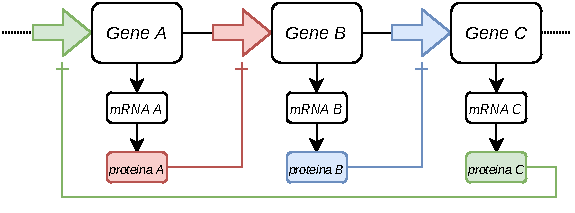
\includegraphics[scale = 1]{img/repr.pdf}
  \caption{Schema di base del Repressilator, con le frecce bidimensionali che
    rappresentano l'azione di inibizione delle proteine.}
  \label{fig:repr}
\end{figure}
Nel dettaglio del Repressilator le proteine (prodotte dai rispettivi geni che si
indicano con la prima lettera minuscola) sono, in ordine (\textit{A, B, C}):
\begin{itemize}
  \item $TetR$ prodotta dal gene $tetR$
  \item $\Lambda cI$ prodotta dal gene $\lambda cI$
  \item $LacI$ prodotta dal gene $lacI$
\end{itemize}
Il punto fondamentale, come visibile in figura \ref{fig:repr}, è capire che se
sto producendo una grande quantità di una 
certa proteina allora sicuramente non avrò produzione di quella di cui
tale proteina inibisce la trascrizione del gene e così via. Nel nostro caso se
si produce tanta \textit{proteina A} non avremo produzione di \textit{proteina
  B} e di conseguenza avremo produzione della \textit{proteina C}, ma nel
momento in cui questa terza viene prodotta cala la produzione della
\textit{proteina A} comportando la produzione della \textit{proteina B}
etc$\ldots$. Ho, in pratica, un sistema oscillatorio, con 3 proteine che si
reprimono l'una con l'altra.\\
La rappresentazione ``su carta'' di questo comportamento è abbastanza semplice,
come vedremo, modellandola tramite un insieme di equazioni differenziali. Il
problema è passare dalla teoria alla pratica. Questo sistema ``ingegnerizzato'',
di equazioni differenziali, è in grado di confermare quanto visualizzabile poi
tramite esperimenti. \\ 
Vediamo quindi come viene effettivamente costruito il sistema sperimentale
usando delle colonie di E. Coli, sfruttando la loro biologia. Nei batteri il DNA
non è, come detto, racchiuso nel nucleo ma ``circola'' in una regione, detta
\textit{nucleoide}, abbastanza accessibile all'interno del citoplasma. Nei
batteri il DNA circola in forme dette \textbf{plasmidi} quindi potenzialmente si
può sintetizzare un particolare plasmide e inserirlo in un batterio, il quale lo
userà per sintetizzare proteine. Prima è stato comunque pensato il modello
matematico e poi stato effettivamente costruito l'esperimento (al contrario
dell'ordine con cui si stanno ora spiegando quindi). \\
I due ricercatori hanno costruito due plasmidi (di cui per ora non approfondiamo
i dettagli):
\begin{itemize}
  \item un plasmide che codifica il\textit{ Repressilator}, ovvero che contiene
  i 3 geni che codificano le 3 proteine. Prima di ogni gene si ha attaccata una
  \textit{zona di induzione} 
  \item un plasmide che codifica un \textit{Reporter}, che codifica una
  particolare proteina, detta \textbf{green fluorescent protein
    (\textit{Gfp})}. La \textit{Gfp} è una proteina usata spesso in quanto fa si
  che un certo sistema diventi fluorescente, di colore verde, una volta che
  viene illuminato con una certa luce (un laser ad una determinata
  frequenza). Questo plasmide fa si che, quando $TetR$ è presente in abbondanza
  la trascrizione del gene \textit{gfp} viene bloccata e quindi diminuisce la
  quantità di \textit{Gfp}. Quindi, come $TetR$ oscilla per il sistema di
  \textit{mutua repressione}, si vedrà al microscopio un'oscillazione della
  fluorescenza della colonia di batteri. 
\end{itemize}
Ricordiamo che la fluorescenza è in realtà abbastanza comune in natura.\\
Si ha un ulteriore ``trucco''. Se si lascia una colonia di E. Coli senza alcun
controllo si avrebbe che ogni batterio inizierebbe il ciclo per conto suo, in
modo non sincrono, impedendo una corretta visualizzazione della
fluorescenza. Questo trucco è quello di inibire la produzione di $LacI$,
interferendo con la sua espressione, usando
un'ulteriore induttore, detto \textit{IPTG} ($isopropyl
\,\beta\mbox{-}D\mbox{-}1\mbox{-}thiogalactopyranoside$), e ottenendo così la
sincronia delle  
cellule dopo questo impulso iniziale di \textit{IPTG} (che poi decade
velocemente lasciando tutti gli E. Coli nello stesso stato iniziale).
\section{Il Modello Matematico}
Facciamo quindi un passo indietro e vediamo il modello matematico del
Repressilator. A partire dal modello matematico si scelgono le proteine da usare
e il comportamento da ottenere.\\
Per prevedere il comportamento complessivo del sistema ingegnerizzato, si è
quindi scritto un modello matematico che rappresenta la variazione 
dell'RNA e delle proteine espresse.\\
Per farlo indichiamo (\textbf{questo indice va sistemato}):
\begin{itemize}
  \item $\alpha_0$, numero di copie di proteine per cellula prodotte da un certo
  promotore in presenza del repressore
  \item $\alpha$, numero di copie di proteine per cellula prodotte da un certo
  promotore in assenza del repressore (sarebbe $\alpha+alpha_0$)
  \item $\beta$, rapporto tra la velocità di decadimento dell'\textit{mRNA} e
  quella della proteina 
  \item $n$, \textit{coefficiente di cooperatività di Hill} (nel caso del
  Repressilator si ha $n=2$)
  \item $m_i$, i-esimo \textit{mRNA}
  \item $p_i$, i-esima proteina che funge da repressore
\end{itemize}
L'intero sistema viene modellato con \textit{coppie di equazioni
  differenziali}. Si hanno quindi: 
\begin{itemize}
  \item un'equazione che ci rappresenta la velocità di variazione dell'i-esimo
  mRNA:
  \[\frac{\dd{m_i}}{\dd{t}}=-m_i+\frac{\alpha}{1+p_j^n}+\alpha_0\]
  Tale velocità dipende dalla quantità che già si ha di mRNA, dalla presenza
  della proteina che lo reprime (essendo sotto nella frazione al crescere il
  termine tende a zero, mentre al diminuire tende a 1)
  \item un'equazione che ci rappresenta la velocità di variazione dell'i-esima
  proteina che funge da repressore:
  \[\frac{\dd{p_i}}{\dd{t}}=\beta(m_i-p_i)\]
  Tale velocità dipende da quanto mRNA si ha a disposizione meno la quantità di
  proteina che si ha a disposizione in quel dato momento. Maggiore è la
  quantità di mRNA e maggiore è la produzione fino a che la proteina stessa
  non supera un certo livello di quantità, avendo che ``satura''
\end{itemize}
In ordine si hanno, per i geni:
\begin{table}[H]
  \centering
  \begin{tabular}{c|c|c|c}
    Indice & 1 & 2 & 3\\
    \hline
    \hline
    $i$ & $lacI$ & $ tetR$ & $\lambda cI$\\
    \hline
    $j$ & $\lambda cI$ & $lacI$ & $ tetR$ 
  \end{tabular}
\end{table}
Con ``velocità di variazione'' si intende in pratica un tasso di cambio di
concentrazione delle due \textit{specie molecolari}, ovvero un'entità che
osserviamo nel modello (in questo caso mRNA o proteina). \\
Le concentrazioni si esprimono con l'unità di misura $K_M$, ovvero il numero di
repressori necessari per dimezzare la repressione di un promotore, e il tempo in
$\tau_{mRNA}$, ovvero la velocità di trascrizione dell'mRNA, detto \textbf{mRNA
  lifetime}.
Integrando numericamente le due equazioni differenziali otteniamo un
comportamento periodico.\\
L'esperimento è stato fatto poi osservando come tutto questo diventa osservabile
in una colonia di E. Coli, opportunamente trattata, usando delle foto (dove si è
osservato anche un drift verso l'alto nel grafico oscillatorio a causa del fatto
che la colonia si espande).\\
La conoscenza di tipo matematico deve però essere trasferita in un esperimento
reale che funzioni (e i ricercatori devono essere in grado di manipolare
entrambi gli aspetti, si quello della modellazione matematica che quello più
biologico e chimico). In questo caso per ottenere oscillazioni stabili servono
determinati prerequisiti:
\begin{itemize}
  \item usare inibitori artificiali piccoli, con la cosiddetta \textit{low
    leakiness}. Promotori più corti sono più facili da manipolare e sono più
  ``veloci'' 
  \item la velocità di decadimento di proteine e mRNA doveva essere simile, per
  ottenere l'oscillazione, una meglio: una buona oscillazione. Questo si ottiene
  attaccando \textit{ssrA} ad ogni repressore 
  \item servono curve di repressione piuttosto ``ripide''. Per questo si è
  usato un promotore con multipli \textit{binding sites} (arrivando alla scelta
  di quelle date proteine), usando repressori
  cooperativi (questo è rappresentato con il parametro $n$) 
  \item usare un \textit{Reporter} non stabile, attaccando una variante di
  \textit{ssrA} a \textit{Gfp}, altrimenti si avrebbe una fluorescenza costante
\end{itemize}
% \begin{figure}[H]
%   \centering
%   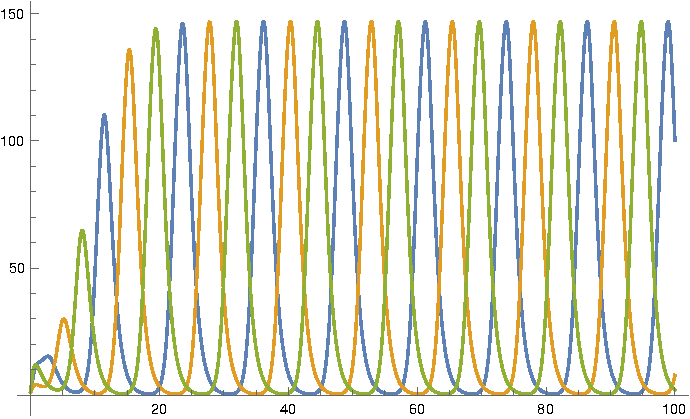
\includegraphics[scale = 0.55]{img/reprprot.pdf}
%   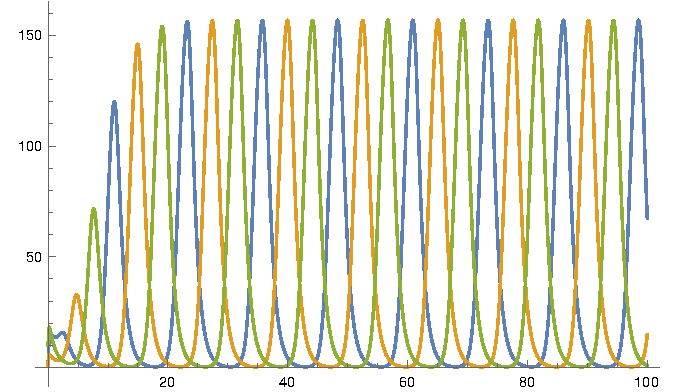
\includegraphics[scale = 0.55]{img/reprmrna.pdf}
%   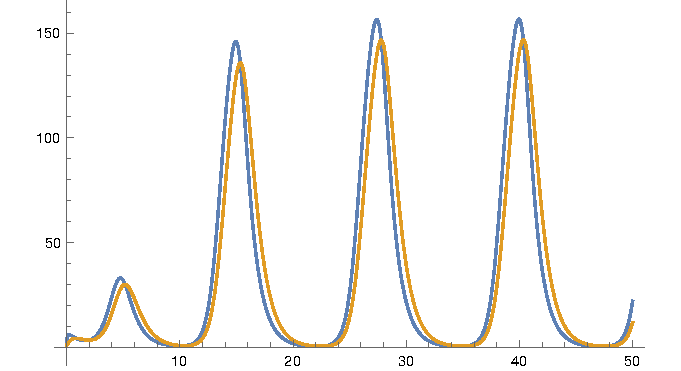
\includegraphics[scale = 0.55]{img/reprmix.pdf}
%   \caption{Grafici relativi al modello del Repressilator ottenuti tramite
%     Mathematica. In primis, a sinistra la quantità di 
%     repressore/proteina rispetto al tempo, a destra quella di mRNA (nel primo
%     caso per le 3 proteine e nel secondo per i 3 mRNA). I grafici
%     cambiano drasticamente quando l'insieme dei valori dei parametri viene
%     modificato. In basso le quantità di mRNA (nel caso di $tetR$) rispetto al
%     repressore/proteina (in questo caso ovviamente $TetR$) associata rispetto al
%     tempo. Si nota che c'è un piccolo delay nel grafico, che rappresenta il
%     tempo di traduzione. Le scale dei tre grafici sono indicative. I parametri
%     sono specificati nel notebook di Mathematica presente nella pagina Moodle.}   
% \end{figure}
\begin{figure}[H]
  \centering
  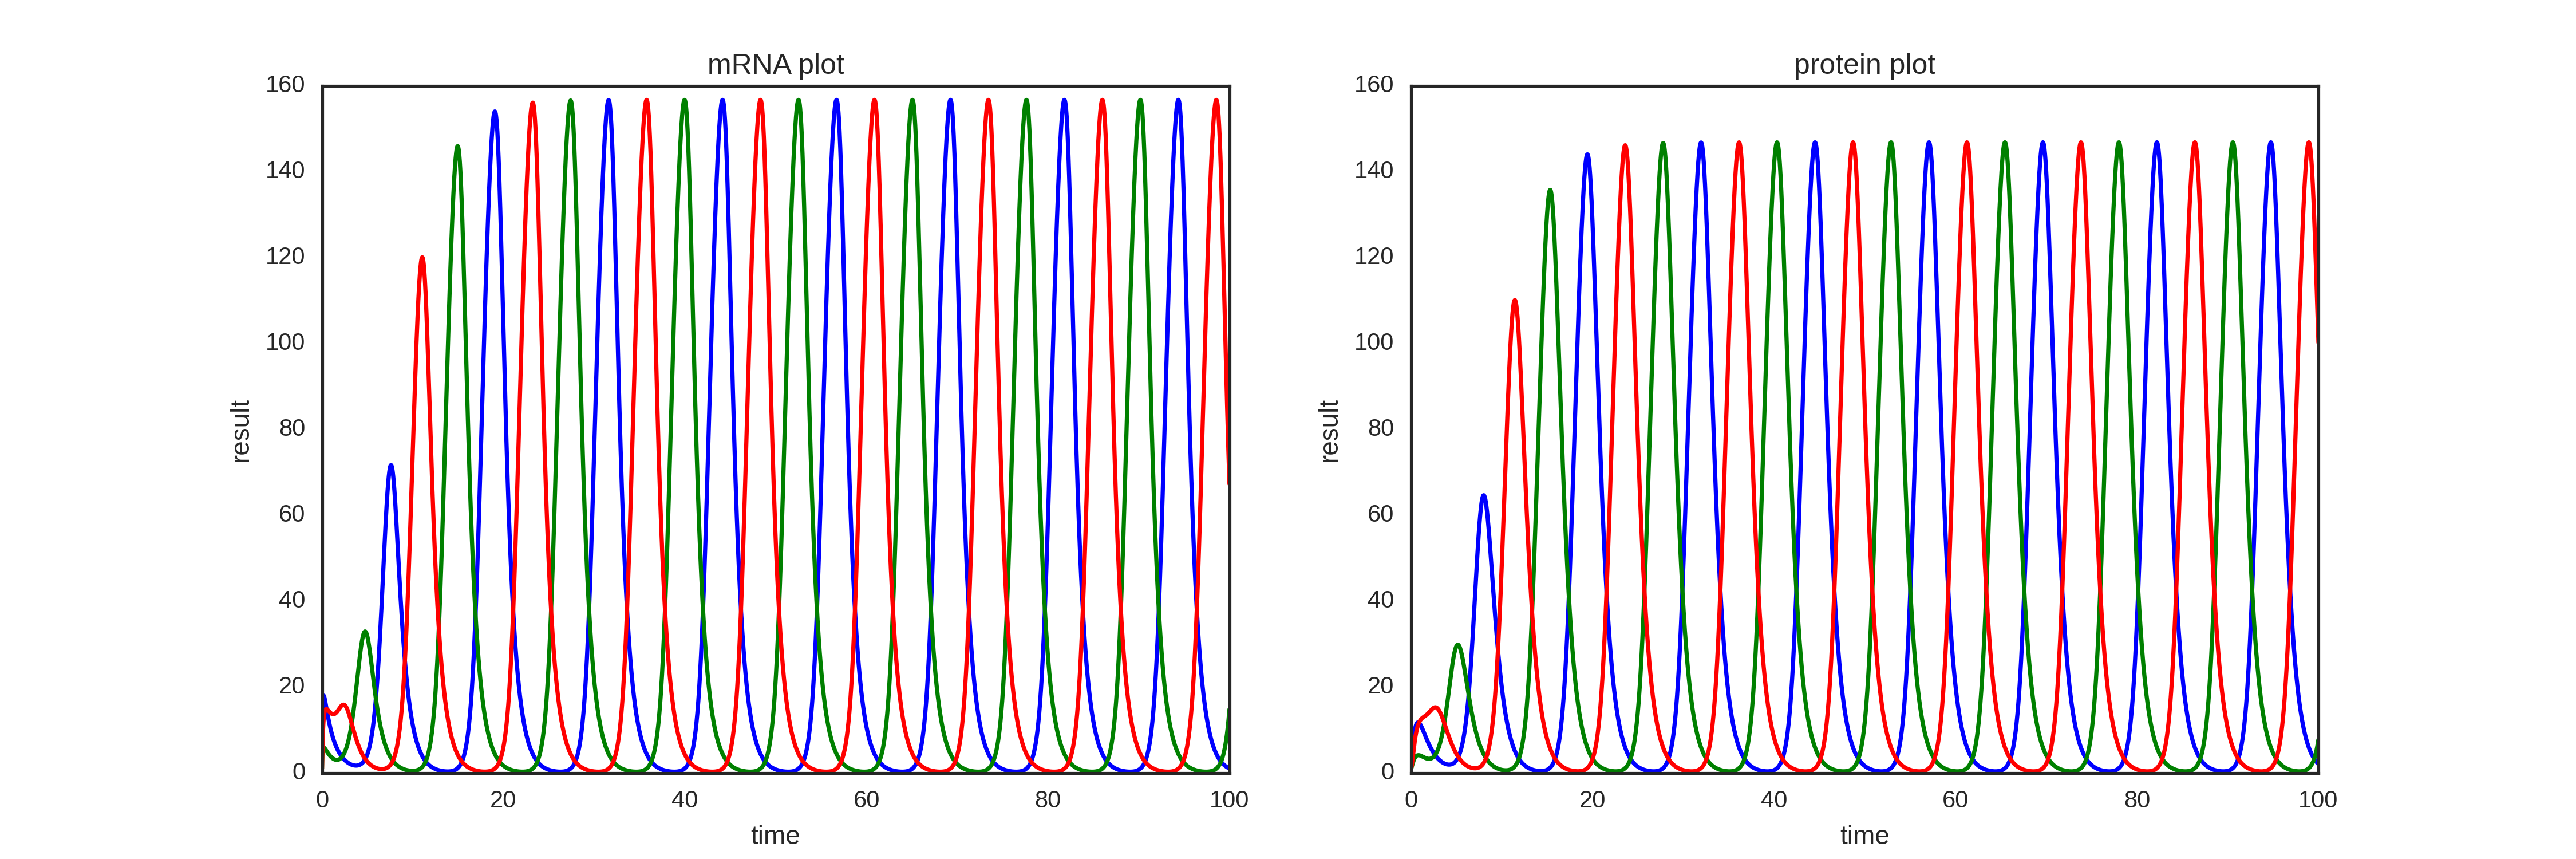
\includegraphics[scale = 0.35]{img/mrna-prot.png}
  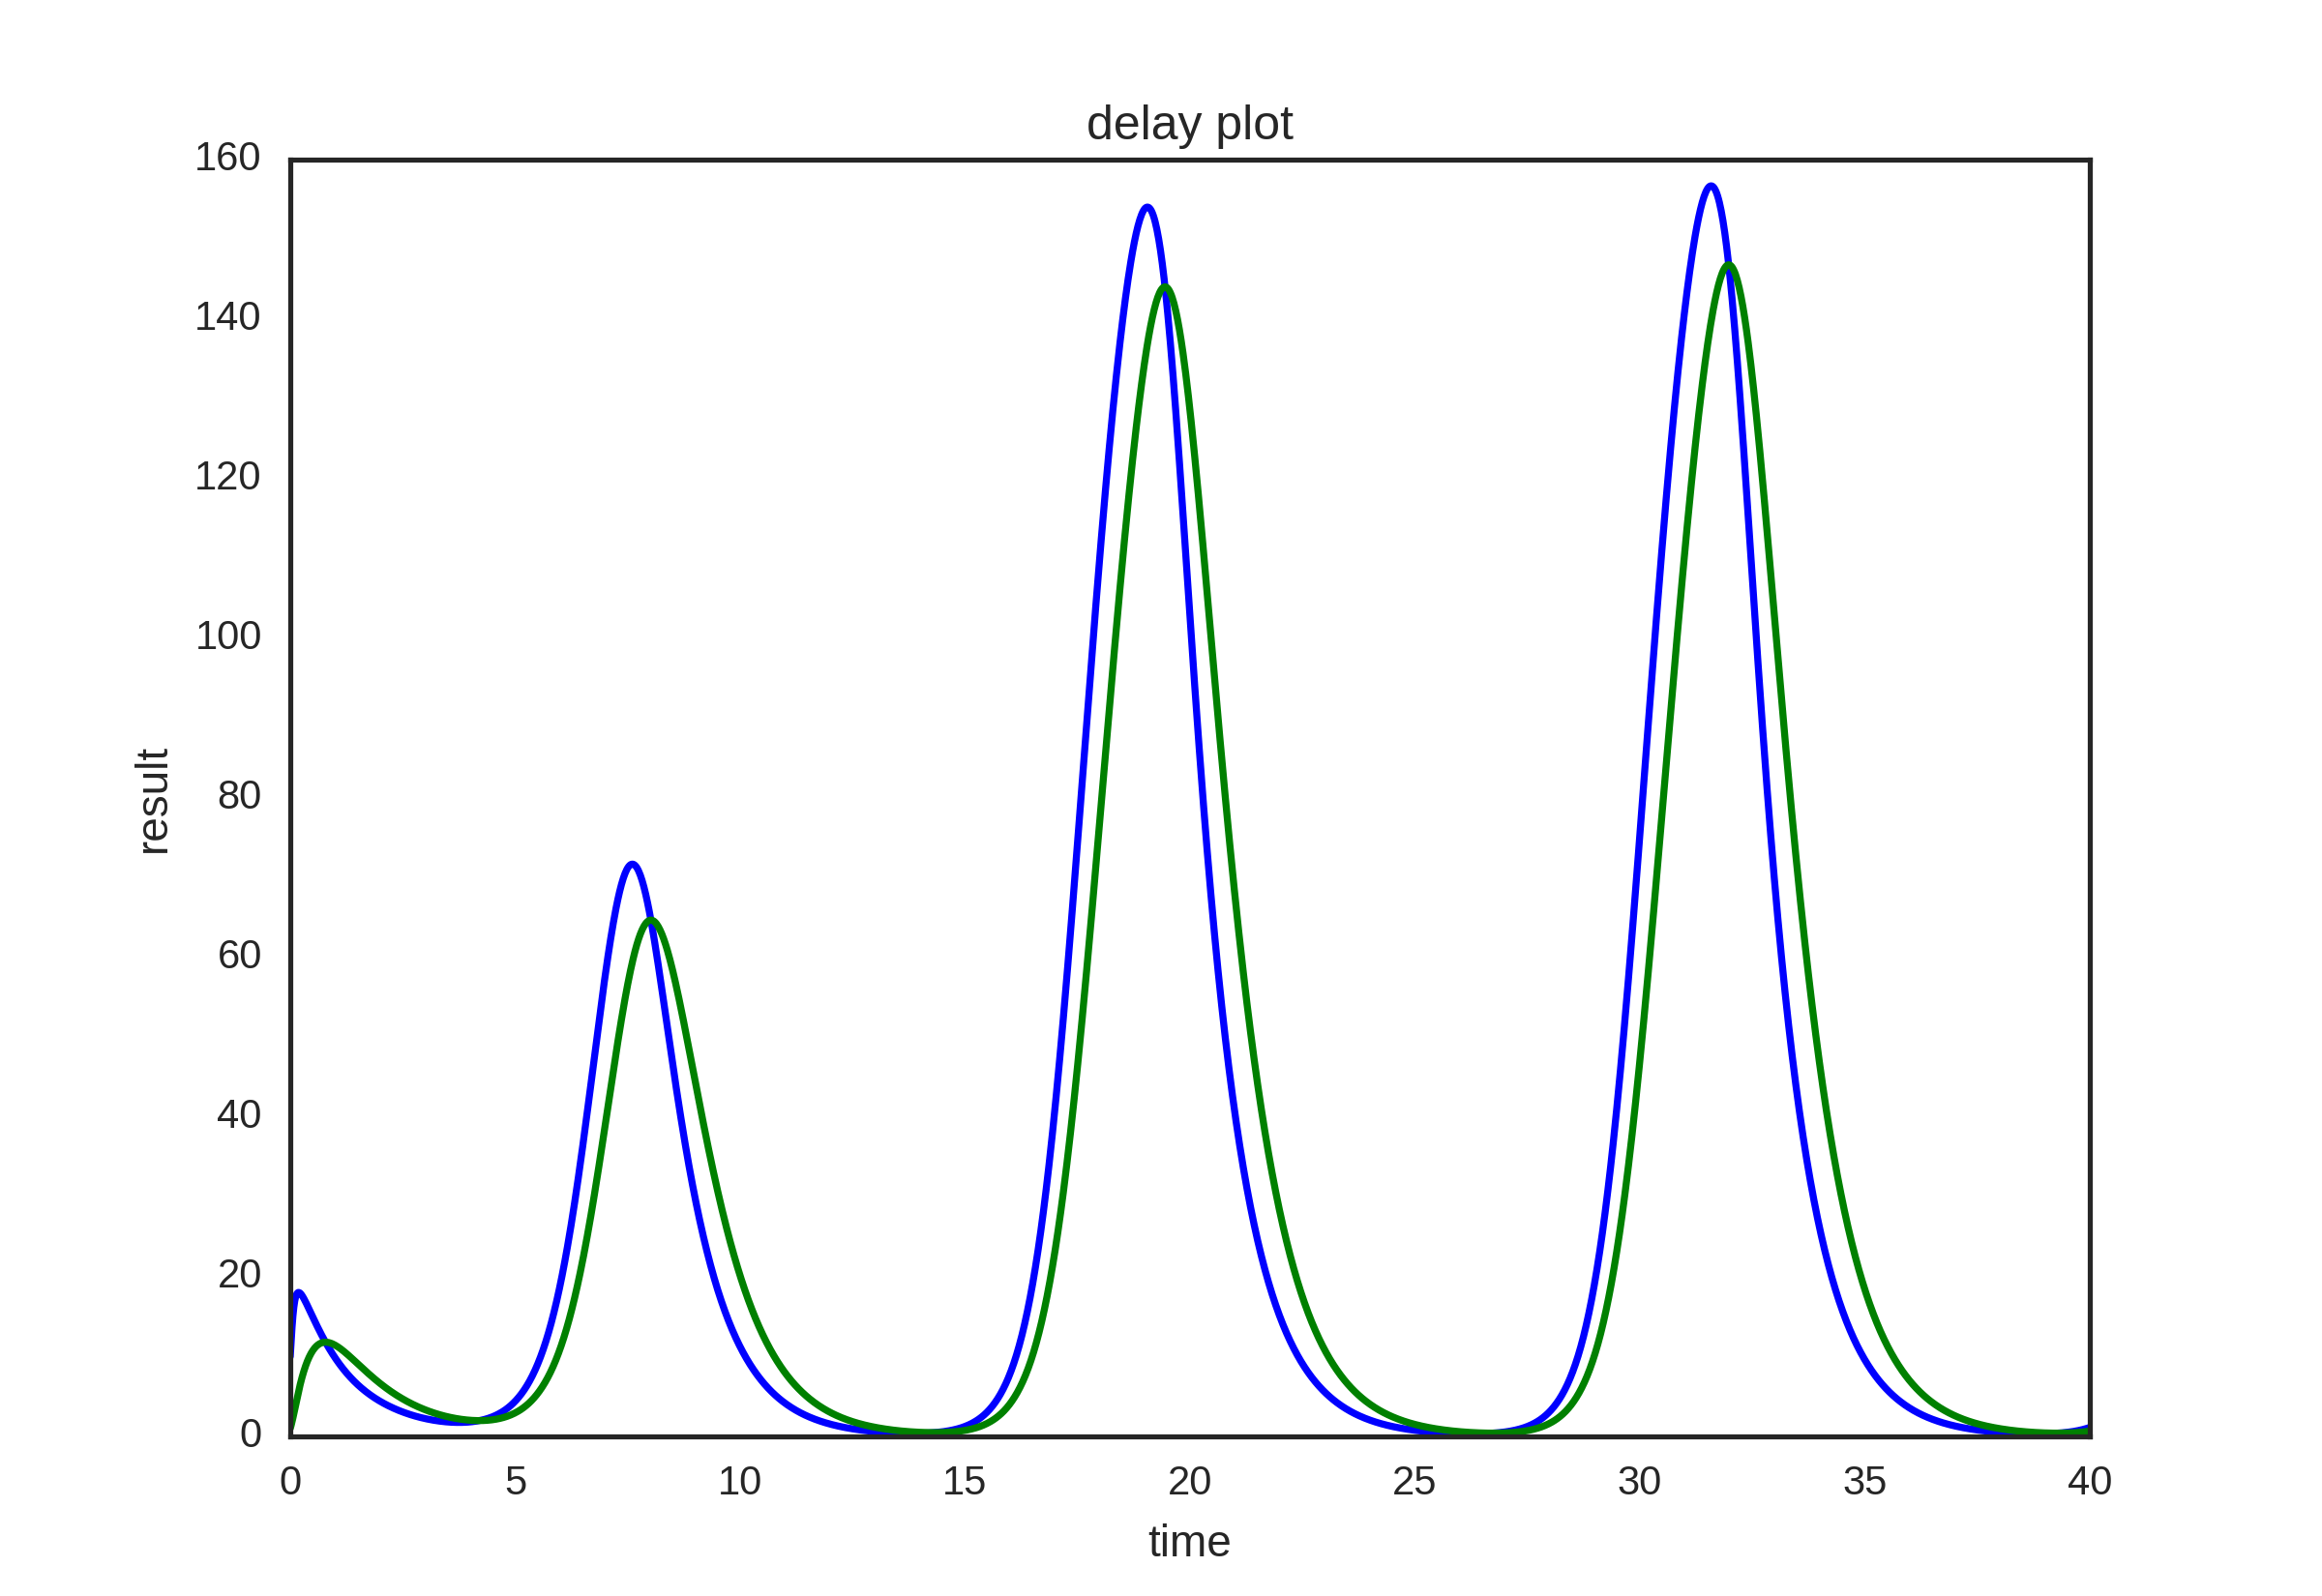
\includegraphics[scale = 0.35]{img/delay.png}
  \caption{Grafici relativi al modello del Repressilator ottenuti tramite
    Python e Matplotlib, con $n=2$, $\alpha_0=0.005$, $\alpha=220$ e $\beta=2$. In
    primis, a destra quella di mRNA mentre a 
    sinistra la quantità di repressore/proteina rispetto al tempo. In basso le
    quantità di mRNA (nel caso di $tetR$) rispetto al repressore/proteina (in
    questo caso ovviamente $TetR$) associata rispetto al tempo. Si nota un
    piccolo delay, che rappresenta il tempo di traduzione.}     
\end{figure}
\begin{listing}
  \begin{minted}{python}
    def repr(var, time, n):
      mRNA = var[:3]
      prot = var[3:]
      dmRNA0 = - mRNA[0] + alpha/(1 + prot[2]**n) + alpha0
      dmRNA1 = - mRNA[1] + alpha/(1 + prot[0]**n) + alpha0
      dmRNA2 = - mRNA[2] + alpha/(1 + prot[1]**n) + alpha0
      dprot0 = - beta*(prot[0] - mRNA[0])
      dprot1 = - beta*(prot[1] - mRNA[1])
      dprot2 = - beta*(prot[2] - mRNA[2])
      return [dmRNA0, dmRNA1, dmRNA2, dprot0, dprot1, dprot2]
  \end{minted}
  \caption{Semplice implementazione del sistema in Python dove l'unico parametro
  che varia è $n$ mentre gli anni sono stati precedentemente fissati}
\end{listing}
\chapter{Studio di Sistemi Biologici}
Cerchiamo ora di capire come classificare i problemi, come analizzarli e
comprenderli (anche tramite machine learning) e avere coscienza delle risorse
online disponibili per la tematica.\\
Buona parte della ricerca in biologia computazionale ha come obiettivo quello di
ottenere il passaggio dai risultati di laboratorio alle applicazioni cliniche
(ed è qualcosa di molto complesso). Per quanto ci sia interesse verso tutte le
patologie la più interessante e più studiata (soprattutto in questo corso) è il
\textbf{cancro} (ma si avrà anche un approfondimento di situazioni pandemiche
come quella del \textbf{Covid}). Un esempio di un sistema particolare dove i
tumori si 
sviluppano è quello delle cosiddette \textbf{cripte coloniche (\textit{colonic
    crypts})}, avendo che questo sistema è relativamente semplice da studiare
dal punto di vista computazionale.\\
Le \textit{cripte coloniche} si trovano nell'intestino e sono delle sorta di
``pozzetti'', morfologicamente divisibili in varie aree.
Alla base delle cripte ci sono delle \textbf{cellule staminali epiteliali}, che
sono quelle che poi danno luogo ai tessuti dell'epitelio. Nella parte più
esterna, ovvero nella superficie intestinale, si hanno le strutture per
l'assunzione dei nutrienti.\\
\textit{Dal punto di vista matematico tutti gli essere viventi sono di topologia
isomorfa a dei tubi.}\\
Tornando al discorso delle cellule staminali si ha che essere si suddividono e,
man mano che si suddividono tendono a spingere verso l'alto le cellule che si
trovano ``al di sopra'' di loro, spingendosi verso la superficie
dell'intestino. Man mano che tali cellule vengono spinte 
anch'esse tendono a dividersi spingendo le altre cellule verso il \textit{lumen
  della cripta}. In questo processo di suddivisione queste cellule si
differenziano e le cellule staminali danno luogo ad una progenie che possiamo,
dal punto di vista in primis computazionale, rappresentare come un
\textit{albero}. Si hanno le cellule di tipo diverso, più o meno
differenziate che continuano a salire verso la superficie dell'epitelio e poi
tendono a salire su quelli che sono detti i \textit{villi intestinali}. Nel
salire si possono produrre situazioni di sovra-riproduzione, provocando la
produzione dei cosiddetti \textbf{polipi}. Questo è
un interessante processo che può essere simulato, tra i vari modi, in modo tale
che si simuli cosa accade quando le varie differenziazioni non funzionano
perché, ad esempio, si ha una cellula che ha acquisito una mutazione, mutazioni
che danno luogo ad una crescita non corretta, ad una \textit{displasia}, che è
la fase iniziale da cui poi si sviluppano i \textit{tumori del colon}. Si vuole
quindi fare queste simulazioni e farle in modo il più fedele possibile. Il
modello delle cripte coloniche è comodo in quanto richiede poche cellule per la
sua simulazione.\\
Per capire se una cellula si sta comportando in modo corretto o meno dobbiamo
misurarne il comportamento. In primis vogliamo misurare due cose, tra le tante:
\begin{enumerate}
  \item \textbf{gene expression}
  \item \textbf{gene alterations}, ovvero le varie mutazioni del genome, le
  cosiddette le \textit{copy number variations} etc$\ldots$
\end{enumerate}
La tecnologia a disposizione per queste tematiche si è molto evoluta ma tra le
tante tecnologie si segnalano:
\begin{itemize}
  \item \textit{microarrays} per l'espressione genica, usati però molti anni fa
  essendo una delle prime tecnologie per misurare, in modo indiretto ma
  parallelo, l'espressione dei geni
  \item \textit{Next Generation Sequencing (NGS)} per praticamente qualsiasi
  cosa, anche per l'espressione genica, in modo diretto tramite particolari
  esperimenti (\textbf{nella rec non ho capito il nome di tali
    esperimenti}). NGS ha avuto molta fama da circa il 2006 in poi, con il
  monopolio poi di Illumina, anche se di recente si hanno nuove tecnologie che
  stanno rivoluzionando il settore (che producono read più lunghe)
\end{itemize}
\section{Microarrays}
Parliamo un secondo dei \textbf{microarrays}.\\
Questa è una tecnologia non più utilizzata, essendo di inizio anni duemila, che
però è utile per spiegare come si procede a fare un certo tipo di misure, con
una tecnologia che è stata poi ripresa da Illumina.\\
Questo strumento si basa su una griglia a cui sono attaccate delle ``sonde''
lunghe circa 25 nucleotidi e venivano usati per caratterizzare i geni. Si
producono infatti segnali luminosi di diversa intensità e diversa lunghezza
d'onda in una griglia, da cui si può ricavare una griglia numerica che dà
informazioni in merito alla luce di ogni punto.\\
I Microarrays sono prodotti da Affymetrix e hanno circa $10^5$ sonde, che
caratterizzano tutti i geni che interessano e l'attacco alle sonde avviene
tramite basi complementari. \\
Si ottiene quindi un'immagine contiene una griglia, dove in ogni punto si
produce un segnale luminoso di diversa intensità e lunghezza d'onda dalla quale
si ricava, misurando i segnali luminosi, una \textbf{matrice di espressione},
dove:
\begin{itemize}
  \item le righe sono i geni/trascritti
  \item le colonne sono misure numeriche
\end{itemize}
e si ha, per ogni sonda, quanto e come è luminoso il tal punto nella griglia.\\
Si prende quindi del DNA, lo si ``denaturalizza'', ovvero lo si sgroviglia, e lo
si versa direttamente sulla griglia. Il DNA (ma potrebbe essere anche essere
RNA) viene versato sulla griglia e si ``attacca'', grazie alle sue proprietà
chimiche, alle sonde (in pratica le parti di DNA/RNA si attaccano alle sonde a
loro complementari). Il trucco è quello di ``colorare'' i pezzi di DNA e RNA e
questo si fa usando, come nel caso del Repressilator, delle proteine
fluorescenti, verdi e rosse, usando quindi processi biochimici per attaccare ai
pezzi di DNA/RNA queste proteine, che emetteranno fluorescenza una volta colpite
da un laser. Si può quindi vedere, in ogni punto della griglia, se si ha un
segnale rosso o uno verde, misurandone l'intensità, ottenendo una misura di
quanto materiale genico si sia attaccato in ogni punto della griglia.\\
Vediamo quindi come si utilizza questo tipo di tecnologia per fare delle misure
di \textit{geni differenzialmente espressi in diverse condizioni}.\\
Si hanno delle cellule in una certa condizione e altre in un'altra condizione
(magari, per esempio, una delle due condizione è una crescita in ambiente con
pochi nutrienti o in un ambiente con temperature estreme, sia alte che basse con
associati shock termici per le cellule). La prima condizione è normalmente uan
\textit{condizione standard}, detta \textit{condizione wild-type}, mentre la
seconda è la condizione che si vuole studiare.\\
Si hanno due fasi per l'esperimento (anche se tendenzialmente non sono
esperimenti molto semplici):
\begin{enumerate}
  \item si estrae dalle cellule nelle due condizioni l'RNA, che descrive ciò che
  le cellule stanno in quel momento esprimendo, quali proteine stanno
  sintetizzando, etc$\ldots$ Dall'RNA, che nel dettaglio è \textit{mRNA},
  estraggo il \textit{cDNA}, al quale poi attacco le proteine per la
  fluorescenza. Si procede quindi con la cosiddetta \textit{ibridazione}, ovvero
  si prende il materiale genetico con fluorescenza e si immerge il
  microarrays in questa soluzione, procedendo poi alla scansione con il
  laser
  \item nella griglia si ottiene quindi che del materiale genico delle cellule
  nella prima condizione si attaccano ad alcune sonde mentre quella delle
  seconda condizione ad altre. In ogni punto della griglia o non si attacca
  niente (non avendo che le cellule esprimono quanto necessario per quel punto)
  o si attacca solo l'RNA di una delle due condizioni o si attaccano entrambi.
  Usando poi i laser per le due fluorescenze si ottiene l'immagine, avendo punti
  senza luce (nero), alcuni con luce verde, alcuni con luce rossa, a seconda
  della prevalenza del materiale che viene da una delle due condizioni (se
  simili si ha una luce tendente al giallo). Una volta prodotta l'immagine si
  produce l'output numerico delle intensità. 
\end{enumerate}
L'esperimento può essere ripetuto più volte, ottenendo una serie di matrici
numeriche che possono unite in vari modi, ottenendo la \textbf{gene expression
  data matrix} finale, coi vari \textbf{gene expression levels}, i livelli di
espressione di ogni gene, ricordando che ogni gene è codificato da più
sonde. Per ogni gene ho la \textbf{differenza di espressione} tra le due
condizioni.
\begin{definizione}
  Si definiscono due geni come \textbf{differenzialmente espressi} se sono due
  geni che risultano rossi o verdi (???).
\end{definizione}
Se tale matrice finale è ottenuta variando solo i tempi e mantenendo 
fisse le altre condizioni sperimentali si ha che essa rappresenta il
\textit{time-course of genes expression}.\\
Sui risultati si può fare \textbf{data mining}, usando tecniche di machine
learning. \\
Si vuole fare clustering di geni o sonde che esibiscono un comportamento simile
dato un insieme di condizioni sperimentali o ambientali. Per farlo si hanno vari
tool (molti dati disponibili sulla repository NCBI, soprattutto nella
sotto-repository GEO) ma molti studi richiedono
una sistemazione finale non banale in merito a ``rumori'' e variazioni di
protocollo nei laboratori. \\
Ad esempio, in un esperimento di espressione genica si hanno vari step:
\begin{enumerate}
  \item dopo la ``pulizia'' della matrice (tramite controllo qualità) si usano
  alcune analisi standard, ragionando magari su vari \textit{time points}
  discreti: 
  \begin{itemize}
    \item \textit{clustering}, tramite K-Means, per ogni punto, ottenendo dei
    vettori che rappresentano il comportamento  di un gene in un certo tempo. Si
    ottengono cluster di traiettorie. Si raggruppano geni con simile profilo di
    espressione 
    \item \textit{enrichment}, che altro non è l'operazione in cui si prendono i
    dati e gli si associano informazioni, tramite \textit{Gene Ontology (GO)
      Terms}. La GO è un elenco di nomi con ID unico e oggi come oggi i geni
    noti sono stati già etichettati coi termini dalla GO. Vengono annotati i
    termini sovrarappresentati in un cluster. L'etichettatura fa si che quando
    ho gruppi di geni posso usare tecniche statistiche, come il \textbf{test
      esatto di Fisher}, per estrarre i termini più rappresentativi, quelli più
    presenti e descrittivi di un gruppo. In 
    questo modo, un cluster può essere associato ad alcuni termini
    ``rappresentativi'', che possono indicare una certa caratterizzazione
    funzionale e ipotesi di associazioni tra geni e un certo comportamento (se
    questo non fosse già annotato). Questa tecnica è detta \textbf{associazione
      a delinquere}, in quanto si ``accusano'' geni di essere associati ad
    altri, comportandosi in modo simile
  \end{itemize}
\end{enumerate}
\textbf{Su slide, parte 2 a pagina 13, grafici di un esperimento e annessi
  termini da GO}.\\  
Vediamo nel dettaglio GO\footnote{\url{www.geneontology.org}}
che è appunto un \textit{vocabolario
  controllato/ontologia} che è diventato la chiave per condividere le conoscenze
biomolecolari, in particolare per i geni e i prodotti genici. Questa ontologia è
nata studiando la \textit{fruit fly}. È nata negli anni
novanta a Berkeley mettendo insieme una serie eterogenea di conoscenze
proveniente da vari ambienti. È nata cercando una nomenclatura standard per la
genetica della Drosophila. È stata ottenuta con lo sforzo di informatici,
biologi, filosofi etc$\ldots$ usando, in primis, l'IA simbolica (usata per le
ontologie, ovvero modi di descrivere in modo simbolico una serie di concetti).\\
Ogni temrine in GO ha un codice numerico univoco.\\
Si hanno tre sotto-ontologie, ognuna con una struttura gerarchica a DAG
(\textbf{su slide immagine di struttura}):
\begin{enumerate}
  \item \textbf{MF} (\textit{Molecular Function}), per le attività biochimiche
  il tipo molecolare
  \item \textbf{BP} (\textit{Biological Process})
  \item \textbf{CC} (\textit{Cellular Component})
\end{enumerate}
Lato tecnico si ha, sotto GO, un linguaggio logico (stile \textit{Prolog}), con
un insieme di relazioni, termini e costanti di un linguaggio.\\
GO non è l'unica ontologia a disposizione, anzi se ne hanno centinaia ma meno
importanti. GO offre delle API e si hanno tool come \textit{AmiGO} o
\textit{PANTHER} per recuperare informazioni.
\section{Next Generation Sequencing}
Dopo aver parlato di \textit{microarrays} parliamo di \textbf{Next Generation
  Sequencing (\textit{NGS})}.\\
Vediamo quindi le nuove tecnologie di sequenziamento. Diciamo ``nuove'' perché
le prime tecnologie di sequenziamento sono datate anni cinquanta con il metodo
Sanger per sequenziare proteine. Più avanti, nei primi anni settanta, si sono
sviluppati i primi progetti per sequenziare DNA e RNA, studiando i virus (in
quanto molto piccoli). Nel 1995 poi si è riuscito a sequenziare interamente un
batterio, l'H. Influenza.\\
Nel 1990 si svilupparono vari metodi per il sequenziamento high-throughput,
progetti che permisero di lanciare lo \textit{Human Genome Project}, che fu
completato nel 2000 quando pubblicarono in estate la prima bozza di genoma
umano. \\
Le prime macchine semiautomatiche per il sequenziamento furono le
\textit{Biosystems ABI 370} ma oggi si usano i macchinari \textit{Illumina}. Un
macchinario \textit{Illumina HiSeq 2000} corrisponde, in termini di prestazioni,
a 23648 \textit{Biosystems ABI 3730}, degli anni novanta.\\
Si hanno due tipi di attività parlando di NGS:
\begin{enumerate}
  \item \textbf{Wet-Lab Activity}, ovvero le attività di raccolta dati/misure
  del materiale biologico, ovvero del vero e proprio sequenziamento tramite
  tecniche biochimiche. Si ha
  quindi la frammentazione e l'estrazione dei frammenti di DNA e RNA, il
  sequenziamento dei frammenti e la generazione delle read (con le 4 basi e
  caratteri extra per le ambiguità o i dati mancanti)
  \item \textbf{Dry-Lab Activity}, ovvero le attività di assemblaggio. Si ha il
  salvataggio delle read, che sono tantissime (con conseguenti problemi di
  storage), e l'assemblaggio delle 
  read (che sono \textit{short read}) in \textit{contings}, che sono read più
  lunghe. Dai contings si passa poi alla sequenza più ampia che stiamo
  sequenziando (anche un intero cromosoma o un intero genoma). Quest'ultimo è un
  problema prettamente algoritmico
\end{enumerate}
Attualmente le tecnologie NGS producono read di lunghezza limitata (Illumina
produce read da 70/150 basi circa) e il costo è
proporzionale al numero delle read prodotte. Il parametro più importante è il
parametro di \textbf{coverage}, ovvero il \textit{depth of sequencing}, ovvero
quante sequenze si hanno che coprono la medesima zona di DNA. Avere un alto
coverage riduce il rischio di errore di sequenziamento ma un alto coverage
implica alti costi e quindi è un parametro che va ``bilanciato''. Sono limiti
tecnologici.\\ 
Il costo di sequenziamento, dal 2006, è sceso di molto e siamo ora intorno ai
1000 dollari per genoma (mentre nel 2000 eravamo intorno ai 100000 dollari). Nel
2006/2007 sono state infatti introdotte le tecnologie Illumina, molto più
economiche. Anche nel 2015 si ha avuto un abbassamento e ora siamo in un
plateau sui 1000 dollari. Inoltre, rispetto alla \textbf{legge di Moore}, il
costo per genoma è sceso molto rispetto alla legge stessa.\\
Si hanno anche nuovi macchinari di sequenziamento, con una diversa tecnologia di
base rispetto ad Illumina:
\begin{itemize}
  \item \textbf{Single Molecule Real Time (\textit{SMRT}) sequencing}, che
  sequenzia una molecola di DNA o RNA per volta
  \item \textbf{Nano Sensing sequencing}, che permette di avere un sequenziatore
  piccolissimo collegabile via USB al proprio computer. Si hanno problemi
  relative al software che ricostruisce le sequenze, avendo percentuali di
  errore veramente molto (con errori di natura diversa da quelli di Illumina,
  che sono comunque percentualmente molto minori)
\end{itemize}
Tra i tipi di sequenziamento abbiamo:
\begin{itemize}
  \item \textbf{Whole-Genome Sequencing}, per interi genomi, anche
  \textit{de-novo} (ovvero senza un \textit{reference} preesistente)
  \item \textbf{Exome Sequencing}, per solo le parti di genoma codificanti
  (infatti solo alcune parti, poche, del genoma codificano le proteine mentre il
  resto del genoma non si sa bene a cosa serva)
  \item \textbf{Target (re)sequencing}, per zone specifiche del genoma, spesso
  sono misure secondarie dopo un Whole-Genome Sequencing per zone ``dubbie'' o
  che servono in quantità maggiore (magari perché legate a certe proteine)
  \item \textbf{RNA-seq}, sequenziando RNA, usando le tecnologie NGS per
  determinare l'attività dell'espressione genica (studiando che proteine sta
  generando una cellula etc$\ldots$), caratterizzando i trascrittomi. Si evitano
  i vari passaggi che si facevano con i microarrays, che davano una misura
  indiretta per di più (l'intensità della luce etc$\ldots$). Qui basta
  sequenziare e poi contare le read di un particolare RNA
  \item si hanno ora molte altre \textbf{*-seq} in letteratura. Ad esempio
  \textbf{ATAC-seq (\textit{Assay for Transposase-Accessible Chromatin using
      sequencing})}, che è legato allo studio della conformazione
  tridimensionale del DNA, delle \textit{aperture/chiusure della cromatina},
  studiando cosa è trascrivibile in un dato istante oppure no
\end{itemize}
\subsection{Dal Sequenziamento alle Analisi}
Dopo il sequenziamento vogliamo vedere come tutte queste informazioni possono
essere usate per fare analisi su come si comportano alcuni processi biologici,
in particolare il \textbf{comportamento dei tumori}.\\
Una delle cose che si possono fare è prendere campioni di tumori da più pazienti
e ricostruire le parti comuni dei tumori stessi, per ottenere i vari sottotipi
del tumore. Questo studio è legato a certi
tipi di tumore (si hanno circa 40 tipi di tumore in totale con i relativi
sottotipi).  \\
Un'altra cosa che si può fare è analizzare il tumore di un individuo che si è
poi suddiviso in \textit{primario} e \textit{metastatico}, costruendo una
\textbf{filogenia tumorale}. Per farlo si prendono campioni del tumore e si fa
una cosiddetta \textbf{bulk analysis}, ovvero un'analisi aggregata prendendo un
tessuto ed estraendo il DNA dal tessuto, ottenendo materiale genico da diverse
cellule (perdendo l'individualità di ogni cellula ottenendo una misura
``media''). Si hanno poi vari algoritmi per ottenere la filogenia, più o meno
complessi, ricostruendo \textbf{l'albero della filogenia tumorale}, che parte da
un tumore iniziale e poi presenta le varie differenziazioni che si sono
sviluppate di quel tumore.\\
Ora si sta sviluppando anche la \textbf{special trascriptomic}, dove si
sequenziano \textit{slice} di tumori tenendo anche in considerazione la
posizione del sequenziamento. 
\section{Single-Cell Analysis}
In merito all'ultimo aspetto della sezione precedente, più di recente, si sono
sviluppate tecnologie più sofisticate dal punto di vista chimico e fisico, per
isolare singole celle prese da un campione. In questo modo si ha una
rappresentazione più precisa di come sono fatte le popolazioni di cellule in un
campione. Si usano poi algoritmi di filogenia per ricostruire le
\textit{evoluzioni clonali}. Questa tecniche sono dette
appunto\textbf{tecniche di Single-Cell Analysis}. Si parte quindi sempre da un
sequenziamento ma associato a singole cellule.\\
La Single-Cell Analysis è cruciale in questo periodo e può essere usata per
tantissimi progetti. In Bicocca si hanno progetti di \textbf{Metagenomica}, dove
si isolano organismi da popolazione di organismi, sequenziando il singolo
organismo (ma sequenziandone tanti). Viene fatto per studiare le popolazioni
microbiche nelle falde acquifere o negli acquedotti. Si isolano organismi noti
da organismi non noti, per riuscire poi a distinguerli e catalogarli,
etichettandoli con il rispettivo materiale genico (il \textit{corredo
  genomico}). Questo non era possibile con questa facilità prima dell'uso della
Single-Cell Analysis. \\
Attualmente è comunque una tecnica molto costosa (contando che in un esperimento
si sequenziano migliaia di singole cellule).
\section{Risorse Online}
Vediamo quindi una breve carrellata di risorse online importanti:
\begin{itemize}
  \item \textbf{NCBI (\textit{National Center for Biotechnology Informationy})},
  dove si hanno tutte le varie risorse più usate, ad esempio \textit{PubMed}
  (per la ricerca di paper), \textit{Blast} (uno dei più famosi allineatori di
  sequenze, nonché uno dei software informatici più usati al mondo),
  \textit{Gene} (un importante database) etc$\ldots$ Si hanno inoltre modalità
  per trasmettere i risultati di ricerche, scaricare dati, informazioni su
  come interfacciarsi senza usare l'interfaccia web (per fare programmaticamente
  analisi più ampie tramite API), varie risorse per imparare le tecnologie,
  tutorial etc$\ldots$ \\
  Dal formato \textit{SBML}, uno standard inspirato \textit{XML}, con cui si
  rappresentano in modo standard i modelli poi si generano gli altri formati,
  tra cui i formati per \textit{MATLAB}
  \item \textbf{BioModels}, dove si trovano modelli di sistemi biologici di
  varia natura (come vari modelli per il Repressilator). Tali modelli sono
  disponibili in vari formati (ad esempio per MATLAB etc$\ldots$) e sono
  simulabili  
  \item \textbf{BioCyc}, un database storico che contiene una rappresentazione
  di tutte le reazioni metaboliche di un organismo. Era nato originariamente per
  il metabolismo di E. Coli ed è stato poi generalizzato a vari organismi
  \item \textbf{KEGG (\textit{Kyoto Encyclopedia of Genes and Genomes})}, un
  portale giapponese che fornisce un insieme di database relativi a vari dati di
  carattere biologico. Fornisce delle API, di recente riscritte per usare la
  terminologia REST, e altri tool
  \item \textbf{Pathway Commons}, un database per pathway metaboliche o
  regolatorie pubbliche
  \item \textbf{Firehose e Firebrowse}, un'interfaccia semplificata ad un
  database complesso chiamato \textbf{TCGA (\textit{The Cancer Genome
      Atlas})}. TCGA è un database, ora parte di NCBI, che raccoglie i dati di
  esperimenti che hanno misurato variazioni nel genoma relativi a tumori, e
  permette di scaricare in modo semplificato i vari dati relativi a tali
  tumori. Si hanno a disposizione vari tipi di studio tra cui, ad esempio, la
  \textit{CopyNumber Analysis}. NOn tutti i tipi di tumori permettono di
  scegliere tutti i tipi di studio, non ancora perlomeno. Si nota che il cancro
  ai polmoni è quello più studiato 
\end{itemize}
Ovviamente questa lista è solo introduttiva.
\chapter{Introduzione ai Prerequisiti}
Prima di proseguire è bene fare una breve digressione sui modelli delle reazioni
chimiche al fine di poterne fare simulazioni tramite modelli matematici. Verrà
quindi fatta una brevissima introduzione di \textbf{biologia molecolare} e di
\textbf{biochimica}, con la rappresentazione di reazioni chimiche e la loro
modellazione. Per farlo verrà ripreso l'esempio del Repressilator.\\ 
In primis conviene riprendere il concetto di \textbf{cooperatività} visto per il
Repressilator, ovvero il valore rappresentato dal \textbf{coefficiente di Hill}
$n$, da cui dipende il dominio dell'oscillazione. Si può quindi ricavare il
coefficiente anche
dall'analisi matematica.. Per capire cosa sia la
\textit{cooperatività} abbiamo bisogno di alcune nozioni di biochimica e di come
le reazioni biochimiche siano state rappresentate nel mondo della computer
science e della bioinformatica. Per cultura personale si elencano alcuni di
questi sistemi:
\begin{itemize}
  \item \textbf{BioNetGen}, un framework di modellazione \textit{rule-based} ed
  esempio di linguaggio standard per modellare sistemi biologici
  \item \textbf{VCell}, un'altra piattaforma di modellazione
  \item \textbf{COPASI}, un software per la simulazione e l'analisi di reti
  biochimiche e della loro dinamica, nato per modelli stocastici ma poi passato
  anche ad altre tipologie
  \item \textbf{SBML}, un \textit{linguaggio di markup} per modellare processi
  biologici 
  \item \textbf{PySB}, una libreria in \textit{Python} per la modellazione di
  sistemi biologici e biochimici mediante modelli matematici
\end{itemize}
\section{Biochimica}
La \textbf{materia} è studiata in varie forme, tra cui, in \textbf{biochimica},
quella di \textit{miscele}. Le miscele possono essere:
\begin{itemize}
  \item \textbf{omogenee}
  \item \textbf{soluzioni} con un \textit{solvente} e un \textit{soluto}. Ci
  sono vari metodi per separare il solvente dal soluto, specialmente metodi
  fisici/meccanici come usare una centrifuga
\end{itemize}
Alcune sostanze non sono però separabili usando semplici tecniche fisiche. Tali
sostanze sono principalmente di due tipi:
\begin{itemize}
  \item \textbf{sostanze pure}, come ad esempio acqua, sale etc$\ldots$ 
  \item \textbf{composti}, come moltissime sostanze in natura
\end{itemize}
Le \textit{sostanze pure} non possono essere separate ulteriormente tramite
tecniche fisiche ma possono essere modificate da reazioni biochimiche. Una
\textbf{reazione} coinvolge un certo numero $n$ di \textbf{reagenti} che portano
ad un certo numero $m$ di \textbf{prodotti}. Le proprietà chimico-fisiche dei
reagenti possono essere modificate e i prodotti della reazione possono essere
composti con caratteristiche molto diverse da quelle dei reagenti. Come
formalismo potremmo avere, 
indicando con $R_i$ i reagenti e $P_j$ i prodotti:
\[R_1\oplus R_2\oplus\cdots R_n\to P_1\oplus P_2\oplus\cdots P_m\]
Ovviamente i prodotti possono essere separabili o diventare a loro volta
reagenti. \\
Ci sono inoltre composti che non possono essere modificati a livello chimico e
questi sono gli \textbf{elementi}. Gli atomi sono l'elemento minimo da
considerare per parlare di 
reazioni biochimiche a livello cellulare e sono composti, come si sa, da:
\begin{itemize}
  \item il \textbf{nucleo}, con \textbf{protoni} e \textbf{neutroni}
  \item gli \textbf{elettroni}, che si trovano in un'orbitale quantizzato. Ogni
  orbitale contiene fino a 8 elettroni (tranne il primo che ne contiene massimo
  solo 2) e quindi si parla di \textit{octet rule}. L'orbitale più esterno è
  \textit{completo} solo nei cosiddetti \textbf{gas nobili} mentre negli altri è
  \textit{incompleto}. Il numero di elettroni nell'ultimo orbitale
  rappresenta la \textbf{valenza dell'atomo}
\end{itemize}
La configurazione dell'orbitale più esterno permette agli stessi di legarsi in
composti. Le \textbf{molecole} sono i composti più piccoli e, se divise,
cambiano le loro proprietà chimiche. La struttura delle molecole dipende
dagll'organizzazione degli elettroni dell'ultimo orbitale condivisi dagli atomi.
Gli atomi con valenza fino a 4, detti \textbf{donors}, tendono a donare
elettroni agli atomi con valenza da 5 a 7, detti \textbf{receptors}, che si dice
hanno una \textbf{tendenza elettronegativa}. \\
Uno strumento essenziale in tale ambito è la \textbf{tavola periodica}. La
tavola periodica ci fornisce informazioni su ogni  elemento conosciuto in
natura, nonché i nuovi elementi sintetizzabili in esperimenti nucleari.\\
Si hanno vari modi in cui gli atomi \textit{legano} tra loro:
\begin{itemize}
  \item \textbf{legame ionico}, tra atomi con una valenza molto diversa (ad
  esempio \textit{NaCl}, dove \textit{Na} ha valenza 1 e \textit{Cl} ha valenza
  7)
  \item \textbf{legame covalente}, tra atomi con una valenza simile (questo
  succede spesso con molecole di atomi dello stesso tipo, come $Cl_2$)
  \item \textbf{legami doppi}, possibili in altre configurazioni (ad esempio
  Carbonio di valenza 4 e due atomi di Ossigeno, che, a loro volta, in coppia
  comportano valenza 4, condividono due coppie di
  elettroni per formare la $CO_2$)
\end{itemize}
Un altro concetto importante è quello di \textbf{polarità}. Le molecole hanno
una polarità, a seconda dell'elettronegatività di ciascun atomo partecipante e
della loro configurazione spaziale. Ad esempio:
\begin{itemize}
  \item le molecole risultanti dai legami tra $O$ e $H$ tendono ad essere
  \textit{polari}, poiché l'elettronegatività di $O$ e $H$ è abbastanza diversa 
  \item le molecole risultanti dai legami tra $C$ e $H$ tendono invece ad essere
  \textit{non-polari}, poiché l'elettronegatività di $C$ e $H$ è simile 
\end{itemize}
Molecole polari tendono ad \textit{attrarsi} mentre quelle non-polari a
sono \textit{neutre} (ad esempio l'acqua è polare mentre olio è non-polare). Nel
dettaglio, le molecole che non si mischiano bene con l'acqua sono dette
\textbf{idrofobiche}.\\
Le forze che creano i legami tra gli atomi sono anche responsabili
dell'\textit{attrazione} tra atomi e molecole. Tra esse si ha la \textbf{forza
  elettrostatica} che agisce tra atomi e molecole. Un'altra forza è la
\textbf{forza di Van der Waals (\textit{vdW})} che, a causa di effetti
quantistici, attrae le molecole a ``lunghe'' distanze e allontana quelle a
``corte'' distanze. \\
Una forza di attrazione intermedia è quella risultante dal cosiddetto
\textbf{legame a idrogeno}. Legami di questo tipo sono essenziali in biologia
(basti vedere il DNA e il legame tra le basi azotate, come in figura
\ref{fig:hyd} e \ref{fig:hyd2}) in quanto il Carbonio è abbastanza
elettronegativo da essere un \textit{donor} per il \textit{legame a
  idrogeno}. Tale legame è quello che viene ``rotto'' con la
\textbf{polimerasi}.\\ 
I legami ionici, covalenti e doppi sono \textbf{legami forti} mentre il legame a
idrogeno, la forza di Van der Waals e la forza elettrostatica sono
\textbf{legami deboli}.\\
\begin{figure}
  \centering
  \chemname{\chemfig{!{guanine}}}{Guanina}
  \qquad
  \chemname{\chemfig{!{cytosine}}}{Citosina}
  \chemmove[-,dashed]{\foreach \i in {1,2,3} { \draw (hb-gua\i) -- (hb-cyt\i)
      ;}} 
  \caption{I tre legami a idrogeno tra Guanina e Citosina}
  \label{fig:hyd}
\end{figure}
\begin{figure}
  \centering
  \chemname{%
    \chemfig{
      N*6([:0](-R)-(=O)-N(-@{b}H)-(=@{d}O)-(-CH_3)=-)
    }
  }{Timina}
  \qquad
  \chemname{%
    \chemfig[shift={(-0.5,-1.25)}]{
      [:90]N*6(-*5(-N(-R)-=N-)=-(-@{a}H_2 N)=@{c}N-=)
    }
  }{Adenina}
  \chemmove{%
    \draw[-,dashed] (a)--(d); 
    \draw[-,dashed] (c)--(b); 
  }
  \caption{I due legami a idrogeno tra Timina e Adenina}
  \label{fig:hyd2}
\end{figure}
\textit{Ogni atomo di carbonio forma 4 legami con altri atomi,
  l'Azoto 3, l'ossigeno 2 e l'Idrogeno 1. Nelle figure delle molecole dove non
si ha nulla indicato si ha un Carbonio.}

\subsection{Biochimica e Metabolismo}
Abbiamo visto come le reazioni biochimiche modificano le proprietà di vari
composti. \\
Una delle reazioni più semplici è quella detta \textbf{dissociazione}. Uno degli
esempi tipici è il sale, $NaCl$, che dissocia in $Na^{+}$ e $Cl^{-}$ a causa
della polarità delle molecole d'acqua. Si noti che questa reazione è
\textbf{reversibile}.\\
Un'altra reazione semplice, stavolta \textbf{irreversibile}, che coinvolge più
composti è la combustione dell'Idrogeno, che potremmo scrivere come:
\[2H_2+O_2\to 2H_2O\]
\textit{Il rapporto quantitativo tra i composti in una reazione è chiamato
  \textbf{stechiometria della reazione}} e l'\textbf{energia} è la chiave di
questi ragionamenti .\\
Per passare dal rapporto espresso con la stechiometria e le unità di misura
della fisica (come i grammi) e viceversa si introduce una nuova unità di
misura. Un esempio famoso dice che:
\begin{center}
  \textit{Un grammo di Mercurio, $Hg$, contiene un numero diverso di molecole 
rispetto ad un grammo di Potassio, $K$.}
\end{center}
I chimici quindi, usando la teoria della \textit{fisica statistica}, hanno
introdotto il concetto di \textbf{mole (\textit{mol})}, definita come la misura
della \textit{quantità di sostanza}. La mole è definita come la quantità di
sostanza che contiene esattamente $6,02214076\times 10^{23}$ entità
fondamentali, essendo questo il valore numerico della costante di Avogadro
quando espressa in $mol^{-1}$. In altri termini è la quantità di sostanza che
pesa esattamente il suo peso molecolare (ad esempio una mole di Ossigeno, $O_2$,
pesa circa $32g$ mentre una di Idrogeno, $H_2$, circa $2g$).\\
Tra le caratteristiche principali di una reazione abbiamo il \textbf{reaction
  rate}, ovvero la \textit{velocità} con cui avviene la reazione stessa. In
chimica la \textbf{cinetica} è lo studio dei vari fattori che influenzano i
\textit{reaction rate}. Tra questi fattori abbiamo:
\begin{itemize}
  \item temperatura
  \item concentrazione di reagenti (nelle reazioni biochimiche con importanti
  effetti biologici spesso la concentrazione di un dato reagente è molto
  piccola) 
  \item $\ldots$
\end{itemize}
Data una reazione, quando la concentrazione di un reagente è molto bassa, o il
\textit{reaction rate} è molto lento, allora si dice che la reazione è
\textbf{cineticamente alterata} (sebbene questo termine sia solo evocativo).\\
Un tipo molto importante di reazione è quello che implica il trasferimento di
elettroni da una molecola all'altra. Queste reazioni sono dette
\textbf{oxy-reduction} o anche \textbf{redox}. Il composto che cede
l'elettrone si dice che viene \textbf{ossidato} (il nome deriva dal fatto che
l'Ossigeno è l'agente ossidante per eccellenza ma non è l'unico) mentre di
quello che lo riceve viene detto che si \textbf{riduce}, ovvero diventa ``più
negativo''.
\subsubsection{Termodinamica}
Si introduce anche qualche concetto di base di \textbf{termodinamica}.\\
Le reazioni possono avven ire se è presente energia e le reazioni in sé
corrispondono ad un cambio di energia nel sistema in analisi. Si ha che
l'energia \textbf{si conserva} e in biochimica anche la quantità complessiva di
materia si conserva. Le reazioni che necessitano energia/calore per avvenire
sono dette \textbf{endotermiche} mentre quelle che generano energia
\textbf{esotermiche}.\\ 
La quantità di energia interna che un sistema termodinamico può scambiare con
l'ambiente è detta \textbf{entalpia}. Essa non può essere direttamente misurata
ma possiamo misurare la sua variazione $\Delta H$, avendo:
\[H=U+p\cdot V\]
con:
\begin{itemize}
  \item $U$ energia interna
  \item $p$ pressione
  \item $V$ volume
\end{itemize}
Non tutta l'energia è disponibile per il lavoro infatti si ha che una parte di
essa viene dispersa e non è quindi utilizzabile. Questa nozione di dispersione è
formalizzata in termodinamica come l'\textbf{entropia} del sistema. Il
cambiamento di energia complessiva del sistema lo possiamo calcolare come:
\[\Delta U=T\cdot \Delta S-w\]
con:
\begin{itemize}
  \item $T$ temperatura iniziale del sistema
  \item $S$ entropia
  \item $w$ lavoro
\end{itemize}
L'energia che è effettivamente disponibile per compiere il lavoro è detta
\textbf{energia libera di Gibbs}, che si calcola come:
\[\Delta G=\Delta H-T\cdot \Delta S\]
Le reazioni biochimiche devono essere fattibili dal punto di vista
termodinamico, avendo quindi, per esempio, che l'energia libera di Gibbs
disponibile deve essere sufficiente per iniziare la reazione. La fattibilità
termodinamica della reazione comunque non implica che essa avverrà
spontaneamente (ad esempio la combustione del Metano è esotermica ma Metano e
Ossigeno si mischiano senza far partire la reazione a temperatura ambiente). Si
ha quindi che una reazione può avvenire solo se si ha $\Delta G>0$ e $\Delta G$
è sufficiente a superare la \textbf{barriera di attivazione} della
reazione. L'energia necessaria per superare tale barriera è detta
\textbf{energia di attivazione} e ogni reazione ha una propria barriera/energia
di attivazione.\\
Durante una reazione l'energia complessiva del sistema cambia. Gran parte
dell'energia di un sistema biochimico è contenuta nei legami tra i vari
composti, avendo quindi la cosiddetta \textbf{energia di legame}. Gli organismi
devono costruire e distruggere questi legami per vivere/riprodursi e possono
farlo anche eseguendo reazioni non termodinamicamente fattibili, quindi
utilizzando energia per superare le barriere di attivazione. Quando si libera
energia per degradare molecole complesse in molecole più semplici si parla di
\textbf{catabolismo} (come nel caso della \textit{glicolisi}) mentre se si
consuma energia per sintetizzare molecole complesse da molecole più semplici si
parla  di \textbf{anabolismo} (come nel caso della \textit{gluconeogenesi}). Gli
organismi, di 
conseguenza, hanno bisogno di effettuare delle reazioni per generare energia e
uno dei modi più comuni è quello di rompere un legame fosfato nell'\textbf{ATP
  (\textit{adenosina-trifosfato})}, ottenendo/liberando \textbf{ADP
(\textit{adenosina-difosfato})}. L'energia contenuta nei legami fosfato
dell'ATP è sufficiente per attivare molte reazione biochimiche anche se non è
sufficiente per molti degli altri tipi di legame presenti in
un organismo. Per acquisire nell'organismo l'energia presente nell'ATP si hanno
vari modi, tra cui nutrirsi o fare la fotosintesi. Anche il \textit{grasso} è un
modo per conservare energia atta alle azioni base: riprodursi, eventualmente
muoversi, mangiare e non morire. Interessante è notare che
le cellule tumorali si rifiutano di fare \textbf{apoptosi}, che è una procedura
di morte controllata utile negli esseri viventi.
\subsubsection{Metabolismo}
Ciò che l'organismo continua a fare per sopravvivere e riprodursi è accumulare
energia per consumare e sintetizzare complessi biochimici e questa attività, che
per lo più avviene nel citoplasma delle cellule, è detta \textbf{metabolismo} e
si hanno due tipologie:
\begin{enumerate}
  \item \textbf{catabolsimo}, ovvero reazioni di decomposizione di vari
  complessi, per lo più acquisiti dall'ambiente 
  \item \textbf{anabolismo}, ovvero la sintesi di complessi
\end{enumerate}
Questa divisione è presente anche nella \textit{GeneOntology}.\\
\textit{Con ``complessi'' qui si intende ``molecole complesse''}.\\
I vari organismi condividono il funzionamento di molte reazioni di base,
parlando quindi di \textbf{metabolismo centrale (\textit{core metabolism})},
mentre i meccanismi specializzati prendono il nome di \textbf{metabolismo
  secondario (\textit{secondary metabolism})}.\\
Un processo molto importante è quello che permette ad un organismo di
``caricare'' molecole di \textit{ADP} con un gruppo fosfato, generando così
\textit{ATP} e per farlo si ha una catena di reazioni (molte delle quali con
alta energia di attivazione o basso reaction rate), ovvero i \textbf{metabolic
  pathways}. Per ``accelerare'' queste reazione gli organismi usano il
meccanismo della \textbf{catalisi}, in quanto un \textbf{catalizzatore} accelera
una reazione o ne riduce l'energia di attivazione senza essere ``consumato''
durante la reazione stessa. Si ha quindi che il catalizzatore è sia un reagente
che un prodotto della reazione complessiva. I catalizzatori sono chiamati
\textbf{enzimi}, agendo su materiali/sostanze dette \textbf{substrati}.\\
Tra i pathway metabolici principali abbiamo (\textbf{su slide immagini dei
  pathways} e della \textbf{Metabolic Map}): 
\begin{itemize}
  \item \textbf{glicolisi}
  \item \textbf{ciclo di Krebs}
\end{itemize}
\section{Modellazione Matematica}
Bisogna capire come modellare matematicamente le reazioni biochimiche. Si
useranno:
\begin{itemize}
  \item la \textbf{legge di azione di massa}
  \item le \textbf{equazioni di Michaelis-Menten}
  \item la \textbf{cooperatività}, mediante l'\textbf{equazione di Hill}
\end{itemize}
Uno dei punti chiave della biologia computazionale è modellare \textbf{reaction
  network (\textit{reti di reazioni})} che si possono anche suddividere in:
\begin{itemize}
  \item \textbf{metabolic network}, con lo studio di reazioni che riguardano
  molecole, proteine etc$\ldots$
  \item \textbf{regulatory network}, con lo studio di interazioni di geni e
  proteine, studiando, promozione della trascrizione, inibizione, etc$\ldots$
\end{itemize}
\textit{L'interazione spaziale a scala ``meso'' tra elementi cellulari separati
  e tra cellule sarà trattata separatamente.}
\subsection{Legge di Azione di Massa}
Partiamo dalla \textbf{legge di azione di massa (\textit{Law of
    Mass-Action})}.\\
La collisione tra due composti chimici, che sia tra due macromolecole o anche
solo tra due ioni, che chiamiamo $A$ e $B$, accade con un certo \textit{reaction
rate} $k$, e produce un composto $C$ come risultato. Indichiamo formalmente
questo con:
\[A+B\stackrel{k}{\to}C\]
Il reaction rate $k$ è dovuto a vari aspetti:
\begin{itemize}
  \item la configurazione geometrica di $A$ e $B$
  \item la temperatura
  \item altri parametri ambientali
\end{itemize}
Inoltre la legge si applica a sistemi che sono \textbf{in equilibrio} e non
sempre è applicabile, ad esempio quando uno dei composti è presente a
concentrazioni molto elevate, infatti in tal caso può essere che gli effetti
risultanti non obbediscano alla semplice relazione che deriva dalla formulazione
della legge. \\
Possiamo riscrivere il formalismo della legge in modo da rimuovere $\to$ e
usare la notazione delle derivate, ottenendo un'\textbf{equazione differenziale
  ordinaria (EDO)}, in inglese \textbf{ordinary differential equation
  (\textit{ODE})}, che sia continua e deterministica. Indichiamo inoltre con
$[X]$ la concentrazione del composto $X$. Otteniamo quindi:
\[\frac{\dd{[C]}}{\dd{t}}=k[A][B]\]
A causa della termodinamica possiamo inoltre considerare \textbf{reazioni
  bidirezionali}:
\begin{center}
  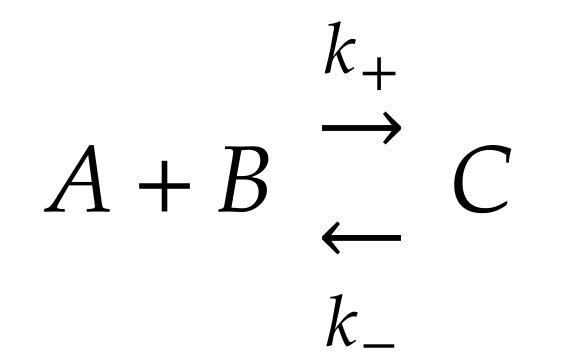
\includegraphics[scale = 0.12]{img/equ.jpg}
\end{center}
Una EDO per queste reazione, ad esempio dal punto di vista di $A$ sarebbe:
\[\frac{\dd{[A]}}{\dd{t}}=k_-[C]-k_+[A][B]\]
Come detto prima vogliamo che il sistema sia in equilibrio in quanto, in tal
caso, le concertazioni dei composti non cambiano e quindi vale la seguente
condizione, data la precedente equazione:
\[\frac{k_-}{k_+}=k_{eq}=\frac{[A]_{eq}[B]_{eq}}{[C]_{eq}}\]
Dove il rapporto $k_{eq}$ è la \textbf{costante di equilibrio} della reazione e,
qualora $k_{eq}$ sia piccolo, si ha indicazione del fatto che $A$ e $B$ sono
state effettivamente ``unite'' in $C$. Si ha che $k_-$ e $k_+$ sono relativi
alla reazione bidirezionale.
\subsection{Equazioni di Michaelis-Menten e Hill}
Passiamo ora a formalizzare la \textbf{cinetica enzimatica}, tramite le
\textbf{equazioni di Leonor Michaelis e Maud Mentes}.\\
Reazioni non elementari, ovvero quelle che non seguono la \textit{legge di massa
di azione}, come ad esempio le reazioni enzimatiche, necessitano la seguente
rappresentazione (con a destra una semplificazione ``empirica'' della stessa):
\begin{center}
  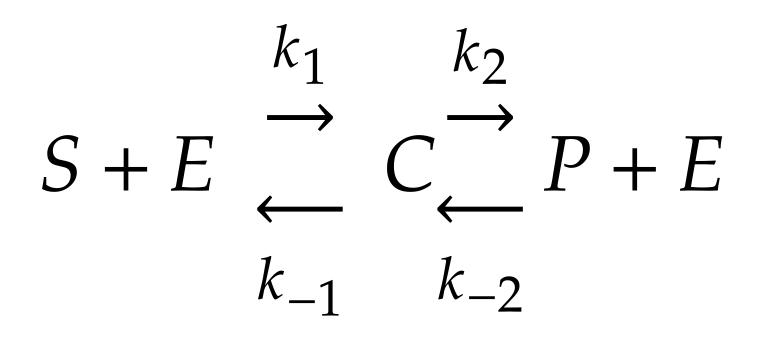
\includegraphics[scale = 0.13]{img/equ2.jpg}
  \qquad
  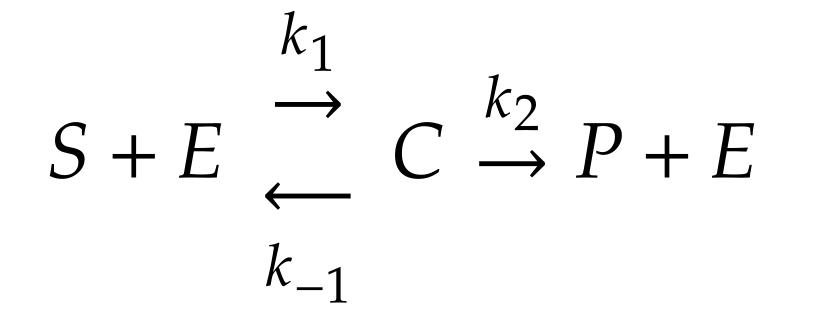
\includegraphics[scale = 0.13]{img/equ3.jpg}
\end{center}
Dove:
\begin{itemize}
  \item $S$ è il substrato
  \item $E$ è l'enzima
  \item $C$ è il prodotto intermedio
  \item $P$ è il prodotto della reazione
\end{itemize}
Quindi da un substrato e l'enzima otteniamo prima un prodotto intermedio con una
prima reazione e poi il prodotto finale con ancora l'enzima, tramite una seconda
reazione, avendo quindi che l'enzima è come se non fosse modificato.\\
Normalmente si considera solo la forma semplificata, la seconda, dove si ha solo
una reazione bidirezionale mentre la seconda diventa
unidirezionale/irreversibile. \\
\textit{Da queste forme possiamo formulare le equazioni di Michaelis-Menten}.\\
L'obiettivo principale di Michaelis e Menten era quello di caratterizzare i
processi di fermentazione, quindi ciò che cercavano erano misure dell'efficienza
di una reazione enzimatica e della sua velocità.  \\
Riprendiamo la formula $A+B\stackrel{k}{\to}C$, e la sua versione
differenziale $\frac{\dd{[C]}}{\dd{t}}=k[A][B]$ per poter ottenere le due
equazioni.\\
Avendo che $[E]_0$ è la quantità disponibile di enzima e che $[E]+[C]=[E]_0$
possiamo riscrivere lo schema della \textit{legge di massa di azione} otteniamo
quattro ODE:
\[\frac{\dd{[S]}}{\dd{t}}=k_{-1}[C]-k_1[S][E]\]
\[\frac{\dd{[E]}}{\dd{t}}=(k_{-1}+k_2)[C]-k_1[S][E]\]
\[\frac{\dd{[C]}}{\dd{t}}=k_1[S][E]-(k_2+k_{-1})[C]\]
\[\frac{\dd{[P]}}{\dd{t}}=k_2[C]\]
Queste quattro equazioni rappresentano la variazione delle quattro ``specie''
considerate rispetto alle altre nel tempo. Si nota che sono le reazioni relative
alla formulazione semplificata in quanto si nota, nella quarta, come $P$ dipenda
solo da $C$ ma non si ha modo di diminuire la velocità di generazione di $P$,
non avendo $k_{-2}$ (nella terza equazione, ad esempio, si vede l'effetto della
bidirezionalità tramite i coefficienti $k$). \\
Consideriamo quindi la concentrazione totale dell'enzima $[E]_0$ (in pratica è
la concentrazione iniziale dell'enzima)
e assumiamo tutti i reaction rate costanti (è un'assunzione non
trascurabile ma semplifica molto il problema). Se osserviamo le precedenti 
equazioni otteniamo che la velocità a cui cresce la concentrazione di $[P]$ è:
\[V=\frac{\dd{[P]}}{\dd{t}}=k_2[C]\approx [E][S]\]
e quindi $V$ è proporzionale alla concentrazione di $[E]$ e $[S]$.\\
Si ipotizza ora che tutto l'enzima $[E]_0$ sia ``esaurito''. A quel punto non
importa se aumentiamo il substrato, non c'è modo di combinare più enzimi e
quindi la velocità della reazione, ovvero la velocità di produzione del
prodotto $P$, raggiunge il suo massimo che chiamiamo
$V_{max}$. Per dire che una reazione può raggiungere una certa $V_{max}$ si
dice che \textbf{satura} a $V_{max}$. \\
Si ha che $\frac{V_{max}}{2}$ la si ottiene ad un certo $K_M$, che è una
concentrazione, che verrà a breve approfondito, come visibile in figura
\ref{fig:km}.\\
\begin{figure}
  \centering
  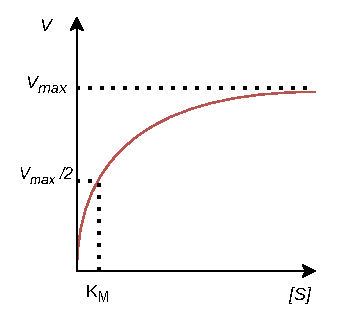
\includegraphics[scale = 1]{img/graph.pdf}
  \caption{Grafico approssimativo rappresentante l'andamento della velocità di
    reazione.} 
  \label{fig:km}
\end{figure}
Il \textit{sistema di Michaelis-Menten} si risolve analiticamente con una
cosiddetta \textit{approssimazione di equilibrio}, con la quale si assume che il
substrato $S$ e il complesso intermedio $C$ sono istantaneamente in
equilibrio. Questo è comodo perché non sempre si possono ottenere delle
soluzioni analitiche (dovendo quindi ricorrere obbligatoriamente a risoluzioni
numeriche) ma in questo caso specifico sì. \\ 
Si ha quindi che si può inferire:
\[k_1[S][E]=k_{-1}[C]+k_2[C]\]
Sapendo poi che $[E]+[C]=[E]_0$, in quanto la quanittà iniziale di enzima deve
essere proporzionale a $[E]+[C]$, avendo che all'inizio, quando ho l'enzima allo
stato iniziale $[E]_0$ ho $[C]=0$. In realtà dovremmo scrivere $[E]+[C]\approx
[E]_0$ ma l'uguaglianza è al momento un'approssimazione accettabile
quindi, avendo $[E] = [E]_0-[C]$ (che sarebbe in realtà $[E] \approx
[E]_0-[C]$), si ha che, sostituendo e raccogliendo:  
\[k_1[S]([E]_0-[C])=(k_{-1}+k_2)[C]\]
e quindi:
\[[S][E]_0-[S][C]=[C]\left(\frac{k_{-1}+k_2}{k_1}\right)\]
Introduciamo quindi il già anticipato $K_M$, che è un combinazione vari di
reaction rate, che nel caso semplificato, con la seconda reazione irreversibile,
è della forma:
\[K_M=\left(\frac{k_{-1}+k_2}{k_1}\right)\]
Facciamo ora un poco di manipolazione delle equazioni già ottenute, ottenendo,
introducendo $K_M$, che:
\[[C](K_M+[S])=[E]_0[S]\]
e quindi:
\[[C]=\frac{[E]_0[S]}{K_M+[S]}\]
Ricordando quindi che la velocità di creazione di $P$, ovvero il reaction rate,
è:
\[V=\frac{\dd{[P]}}{\dd{t}}=k_2[C]\]
Sapendo poi che a $V_{max}$ si ha che che tutto l'enzima $E_0$ deve essere
legato in $C$, si ottiene:
\[V_{max}=k_2[C]=k_2[E]_0\]
Ma allora, rimettendo insieme le varie equazioni facendo le varie sostituzioni:
\[V=\frac{\dd{[P]}}{\dd{t}}=k_2[C]=k_2\frac{[E]_0[S]}{k_m+[S]}=
  \frac{V_{max}[S]}{k_M+[S]}\]
e quindi si ottiene, tenendo solo gli estremi, l'\textbf{equazione di
  Michaelis-Menten}: 
\[V= \frac{V_{max}[S]}{k_M+[S]}\]
Tale equazione ci dice che, se sappiamo la massima velocità della reazione,
siamo in grado di regolare la velocità della reazione stessa (ovvero del
substrato che produce il prodotto finale) semplicemente
andando a modificare la concentrazione iniziale.\\
Michaelis e Menten hanno così potuto regolare i processi di fermentazione della
birra che stavano studiando.\\
Studiamo meglio $K_M$, che è detta \textbf{costante di Michaelis-Menten}. Uno
studio dimensionale sull'equazione di questa costante porta a verificare che è
una concentrazione. Facendo vari conti possiamo arrivare ad asserire che:
\[K_M\approx [S]\]
ovvero si ha che $K_M$ è proporzionale alla concentrazione del substrato.\\
Sostituendo nell'equazione di Michaelis-Menten, si ottiene, come
già in parte anticipato, che:
\[V=\frac{1}{2}V_{max}\]
Si arriva quindi ad una definizione.
\begin{definizione}
  Si definisce $K_M$, detta \textbf{costante di Michaelis-Menten}, come
  la concentrazione del substrato $S$, ovvero $[S]$, tale per cui si ha
  $V=\frac{1}{2}V_{max}$.\\ 
  Questa costante è anche usata per definire la nozione di \textbf{efficienza
    catalitica}, tramite passaggi ulteriori non specificati nel corso. 
\end{definizione}
Possiamo finalmente discutere il significato di \textbf{cooperatività}.\\
Per molti enzimi la velocità di reazione segue la forma di un \textbf{sigmoide},
che è diversa da quella ad \textbf{iperboloide} ottenuta da Michaelis e
Menten con el loro equazioni. Questo accade, ad esempio, quando un enzima può
legarsi a più di un substrato e il primo legame facilita quello
successivo. Questo fatto è stato scoperto sperimentalmente. \\
Ad esempio potremmo avere la seguente situazione, con solo complessi
intermedi $C_1$ e $C_2$: 
\begin{center}
  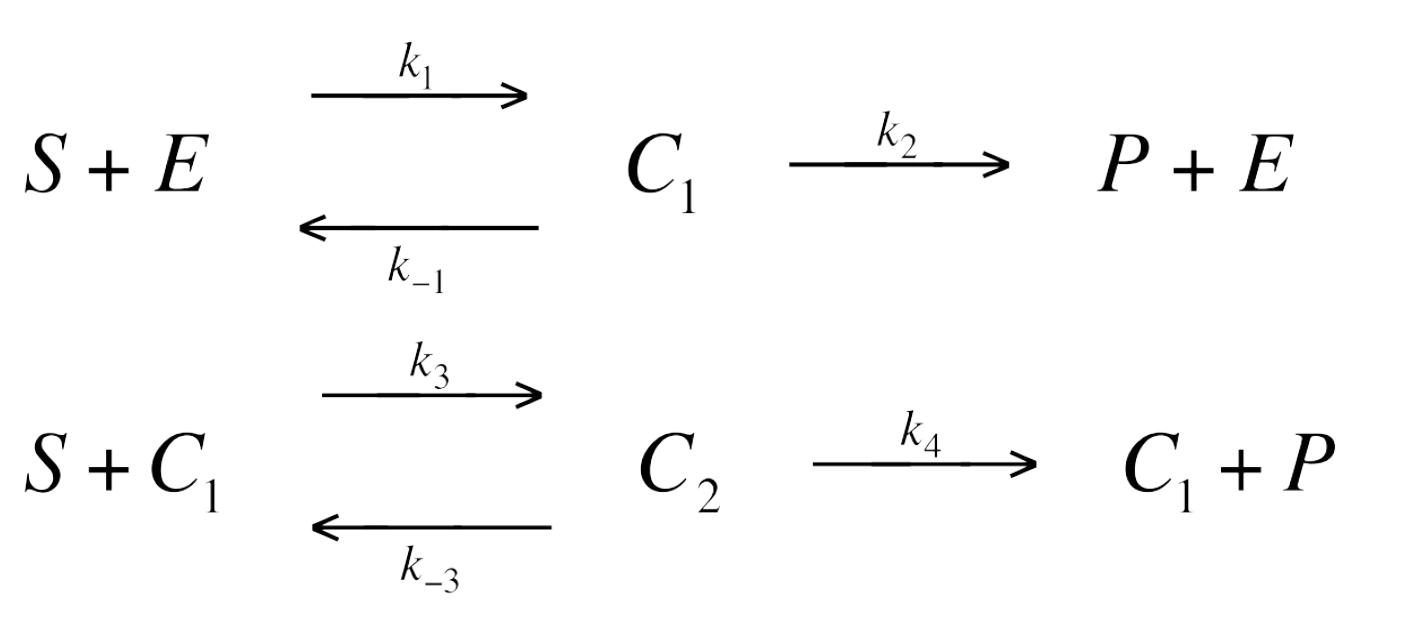
\includegraphics[scale = 0.12]{img/equ4.jpg}
\end{center}
Nella prima reazione  abbiamo la serie di ``passaggi standard'', come già
studiato, mentre nella seconda 
si nota l'intervento del primo complesso intermedio nella reazione che porta al
secondo complesso intermedio, il quale porterà al prodotto finale più ancora il
primo complesso intermedio.\\
Si è modellato quindi un enzima che si può attaccare in più di un modo ad un
substrato, in questo caso abbiamo che si attacca in due modi al substrato
(avendo nel complesso 6 reazioni). 
Ovviamente quello che qui si è visto con due equazioni può essere generalizzato
a $m$ equazioni.
Con altri passaggi matematici potremmo trovare una forma generale per la
velocità, ottenendo l'\textbf{equazione di Hill}, che in questo caso è:
\[V= \frac{V_{max}[S]^n}{K_M^n+[S]^n}\]
con $n$ numero di siti in cui l'enzima può legarsi al substrato $S$ e con $K_1,
K_2, \ldots, K_l$ che sono le $l$ constanti all'equilibrio, avendo che:
\[K_m^l=\prod_{i=0}^lK_i\]
Si noti inoltre che con $n=1$ otterremmo l'\textbf{equazione di
  Michaelis-Menten}.\\ 
L'\textbf{equazione di Hill} è usata per modellare reazioni che si pensa
siano cooperative, ovvero con enzimi che possono legarsi in più di un substrato,
ma i cui dettagli non sono completamente noti. Non si sa come l'enzima si
attacca al substrato ma si stima che dovrebbe farlo in un certo numero di
siti.\\  
A partire dall'\textbf{equazione di Hill} si può tornare al Repressilator e fare
le giuste considerazioni sul coefficiente di Hill $n$.\\
Per fare funzionare comunque un qualsiasi sistema con EDO abbiamo bisogno delle
\textbf{costanti}. Si hanno sostanzialmente due modi per conoscere le costanti:
\begin{enumerate}
  \item si ricercano sperimentalmente in laboratorio di biologia provando
  diverse condizioni in cui avviene una reazione e se ne misura la velocità,
  misurando le concentrazioni prima e dopo un certo tempo, inferendo poi le
  costanti. Per sistemi molto grandi è impraticabile
  \item si usano metodi computazionali per fare \textit{esplorazione dello
    spazio dei parametri}, ovvero il \textbf{parameter sweeps}. Si hanno diversi
  metodi di tipo stocastico o anche metodi più ``controllati'', che danno
  certezza di aver esplorato buona parte dello spazio dei parametri, usando i
  metodi detti di \textit{ricerca su griglia}, ovvero i metodi \textbf{grid
    search}. Anche in questo caso è una ricerca sperimentale dei parametri ma
  dal punto di vista computazionale
\end{enumerate}
Nel dettaglio i parametri $n$, $V_{max}$ e $K_M$ devono essere determinati in
uno di questi modi.\\
Si possono fare alcune considerazioni su $n$:
\begin{itemize}
  \item per $n>1$ si hanno legami che cooperano positivamente, avendo che, non
  appena un \textit{ligando}, ovvero l'enzima, si lega a una molecola,
  l'\textit{affinità di attrazione} per gli altri ligandi aumenta 
  \item per $n<1$ si hanno legami che cooperano negativamente, avendo che, non
  appena un \textit{ligando}, ovvero l'enzima, si lega a una molecola,
  l'\textit{affinità di attrazione} per gli altri ligandi diminuisce
  \item per $n=1$ non si hanno legami che cooperano, avendo che
  l'\textit{affinità di attrazione} dei ligandi non dipende da quanti di loro
  erano già attaccati alla molecola o meno 
\end{itemize}
\textit{In base a quanto detto Elowitz and Leibler scelsero sperimentalmente
  $n=2$, in quanto rappresentava il \emph{comportamento critico} del sistema dal
  punto di vista teorico. Decisero quindi quale tipo di promotori e inibitori (e
  sincronizzatori) utilizzare durante la progettazione del proprio esperimento
  per il Repressilator, portando alla scelta precisa delle 3 proteine usate,
  grazie alla loro conoscenza di biochimica.}\\ 
L'obiettivo di ogni sforzo di modellazione (che mira a modellare, alla fine, le
catene di reazioni, modellate in pathway), infine, è osservare comportamenti
plausibili con l'obiettivo di poter prevedere quelli imprevisti.\\
Per la modellazione si ha un elenco molto esteso di EDO, oltre alle due appena
viste (quella di Michaelis-Menten e quella di Hill), tra cui quelle per il
\textbf{diagramma di Lineweaver-Burk}. Quest'ultima si ottiene a partire
dall'equazione di Michaelis-Menten, facendone il reciproco:
\[\frac{1}{V}=\frac{K_M+[S]}{V_{max}[S]}=\frac{K_M}{V_{max}}\frac{1}{[S]}+
  \frac{1}{V_{max}}\]
È, in pratica, la \textbf{linearizzazione} dell'equazione di Michaelis-Menten e
infatti si ottiene una formula rappresentante una retta, con
$m=\frac{K_M}{V_{max}}$ e $q= \frac{1}{V_{max}}$. Tale retta incontra
l'asse $y$, dove si ha $\frac{1}{V}$, in $\frac{1}{V_{max}}$ mentre l'asse $x$,
dove si ha $\frac{1}{[S]}$, in $-\frac{1}{K_M}$.
\chapter{Simulazioni Deterministiche e Ibride}
Si analizza ora come andare a fare simulazioni tramite equazioni differenziali
ordinarie, le EDO. Si introducono quindi gli algoritmi numerici, i
\textit{risolutori}, per le EDO. Si parla quindi di \textbf{modelli di
  simulazione deterministici}. \\
Parlando di modellazione si hanno varie teorie in uso:
\begin{itemize}
  \item equazioni differenziali, per \textbf{modelli continui}
  \item sistemi discreti, come \textit{automi a stati finiti}, \textit{reti di
    Petri} e \textit{dataflow diagrams} (che non verranno trattati) per
  \textbf{modelli discreti} 
  \item tecniche per \textbf{modelli ibridi}, ovvero modelli continui ma con
  discontinuità e cambi di stato/modalità
\end{itemize}
Un componente importante in tutti i tipi di modellazione è il \textbf{tempo},
inteso come una delle variabili indipendenti del sistema e caratteristica
fondamentale del modello e degli strumenti che si usano per le simulazioni. \\
Una delle cose fondamentali da chiedersi studiano il \textit{tempo} è cosa
costituisce il \textbf{progresso}. Una volta pensato a come modellare il tempo
si ha un modo per capire come procedere a implementare un simulatore
etc$\ldots$. \\
Dal punto di vista computazionale il tempo è \textbf{discretizzato}, come del
resto qualsiasi altra variabile. In ogni caso si classificano i
\textit{framework di modellazione} in base alla loro ``visione di base'' di come
il tempo avanza.\\
\section{Equazioni Differenziali Ordinarie}
Le \textbf{equazioni differenziali ordinarie (\textit{EDO})} sono un modello
standard per modelli fisici, biologici, ingegneristici etc$\ldots$ e assumono un
campo reale dove c'è una variabile, il tempo, reale (e quindi continua).\\
La forma generale di una EDO è:
\begin{gather*}
  \dot{y}(t)=F(y(t),t)\\
  y(t_0)=k
\end{gather*}
$F$ è una funzione, arbitrariamente complessa, che è sia sul tempo che sulla
funzione da calcolare. Si sanno manipolare particolari forme di $F$,
tendenzialmente lineari. Si segnala anche la definizione di $y$ al tempo zero,
data da una costante $k$. Quest'ultima è la \textbf{condizione iniziale} e
bisogna averla per forza. Risolvere l'equazioni differenziale corrisponde a
trovare la forma di $y$ e si dice essere equivalente a \textbf{risolvere un
  problema iniziale (\textit{initial problem solving})}.\\
Riprendiamo, ad esempio, le equazioni del Repressilator:
\begin{gather*}
  \frac{\dd{m_i}}{\dd{t}}=-m_i+\frac{\alpha}{1+p_j^n}+\alpha_0\\
  \frac{\dd{p_i}}{\dd{t}}=-\beta(p_i-m_i)
\end{gather*} 
Dove si hanno, si ricorda 3 copie di equazioni differenziali, relativamente
semplici, al più del $p_j^n$ a denominatore nella prima equazione.
\section{Modelli Discreti}
Nei \textbf{modelli discreti} si ha un'idea molto diversa del \textit{tempo},
avendo una nozione derivata dall'osservazione dell'evoluzione del sistema.\\
Ad esempio con le \textbf{finite state automata (\textit{FSA})} abbiamo una
rappresentazione di come l'evoluzione del sistema possa passare attraverso vari
stati. Con le \textbf{reti di Petri} abbiamo una versione succinta dei FSA con
delle eventuali estensioni. Si usano specialmente reti di Petri che sono
codifiche che dal punto di vista teorico sono più espressive dei FSA, in
quanto si riconosce un insieme di linguaggi che contiene quello riconosciuto
dai FSA.\\
Si ha poi una particolare implementazione di FSA o di reti di Petri, detta
\textbf{Discrete Event Systems (\textit{DES})}, ovvero una rappresentazione
molto ``operativa'' di quei modelli, dove si ha una coda di eventi generata da
\textit{diversi sorgenti} e processata da vari \textit{componenti}. La
generazione degli eventi è normalmente associata ad un tempo, tempo in cui
l'evento accadrà, e se si hanno più componenti bisogna ordinare i vari elementi
generati. \\
Il \textbf{tempo} è normalmente una \textit{nozione derivata} nei modelli
discreti ottenuto da un'osservazione di sequenze di eventi o un'osservazione di
un tempo esterno, rappresentabile a sua volta da un FSA o da una serie di
eventi, parlando \textbf{Wall Clock}.
\subsection{Modellazione di Cellule Staminali}
Vediamo quindi l'uso di modelli discreti per la rappresentazione di una
\textbf{popolazione di cellule staminali}, studiandone \textit{proliferazione}
e \textit{differenziazione}. Nel dettaglio si parla di \textbf{cellule staminali
 ematopoietiche}, ovvero quelle che danno origine a tutte le cellule del
sangue (si hanno infatti vari tipi di cellule staminali, come quelle neurali,
quelle muscolari, quelle epiteliali etc$\ldots$).\\ 
Una cellula staminale si differenzia in una serie di possibili \textbf{cellule
  progenitrici} che sono più differenziate e che infine si differenziano
totalmente in cellule ``finali'', nel caso del sangue, in analisi:
\begin{itemize}
  \item cellule T
  \item globuli rossi
  \item $\ldots$
\end{itemize}
Con \textbf{sistema ematopoietico} si intende il sistema che da luogo alle
cellule che compongono il nostro sangue. Le cellule ematopoietiche derivano
dalle \textbf{cellule stromali} contenute nel \textit{midollo osseo}.\\
Modellazione del sistema in figura \ref{fig:schema}
\footnote{\url{https://stemcells.nih.gov/info/Regenerative_Medicine/2006Chapter2.html}}
\begin{figure}
  \centering
  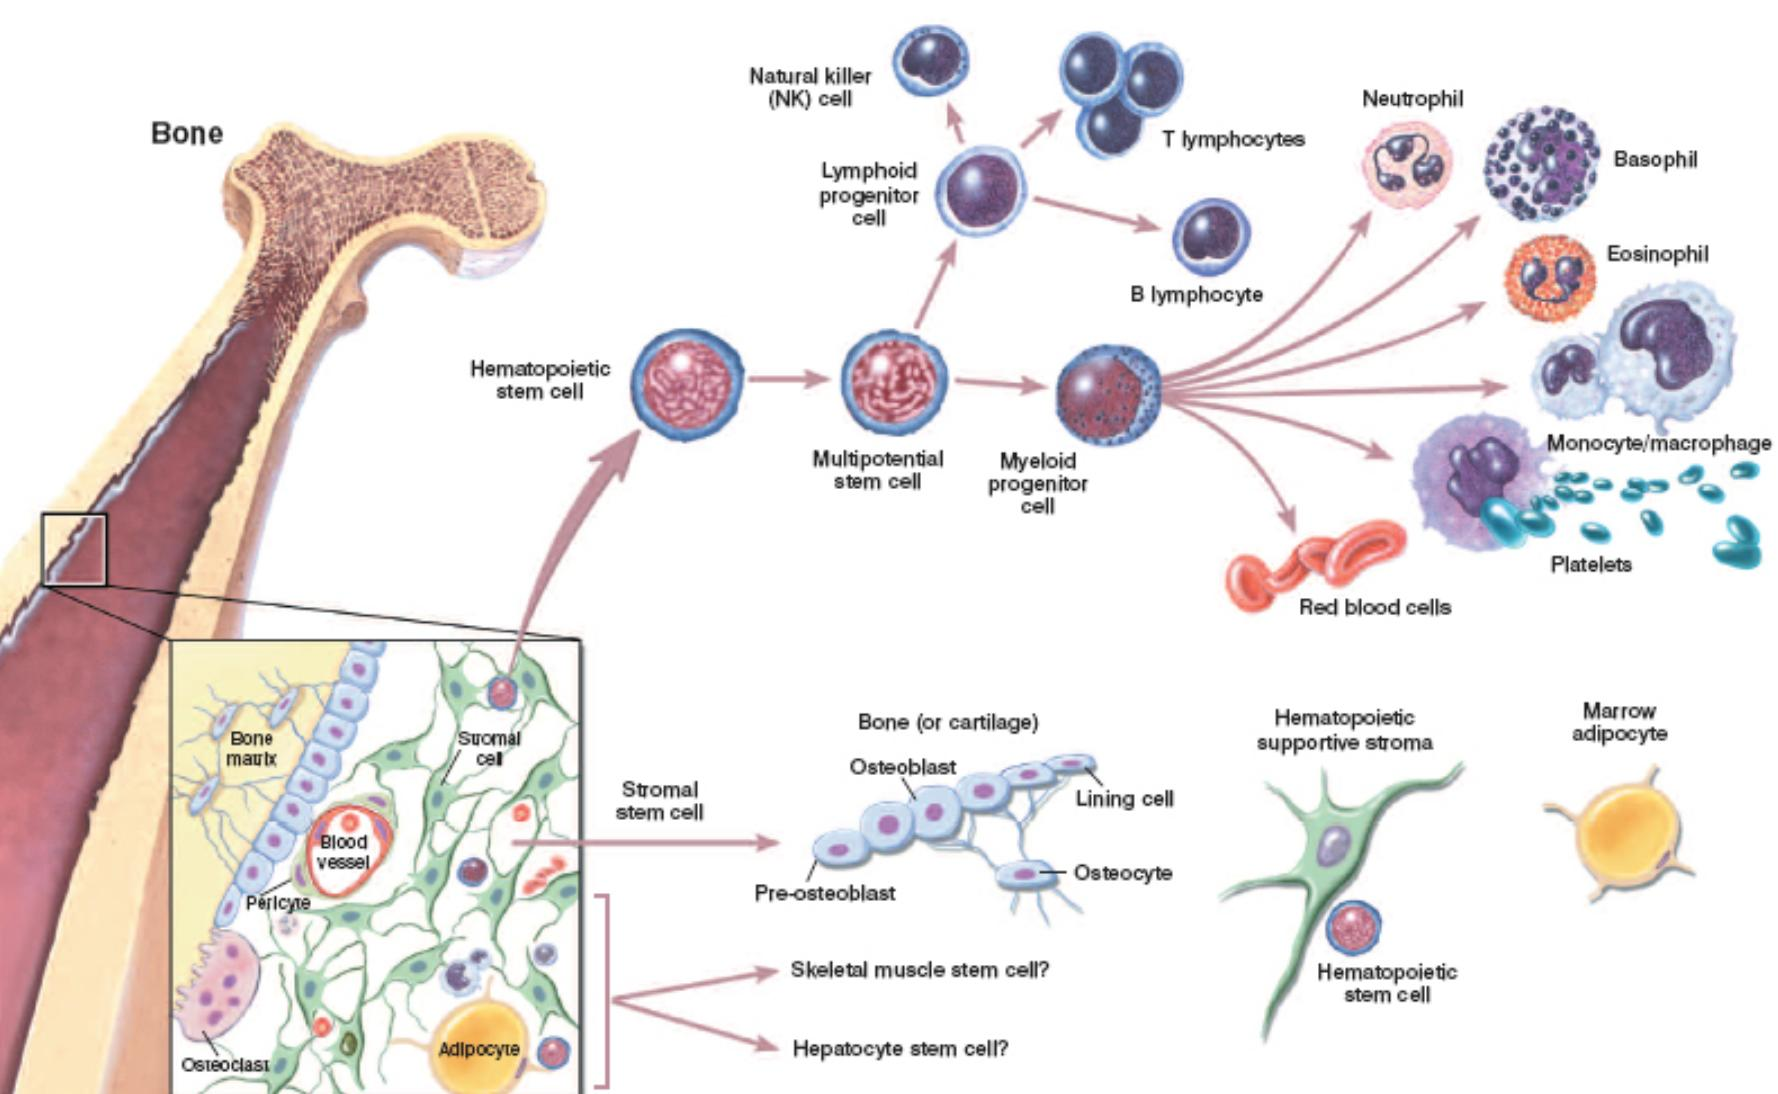
\includegraphics[scale = 0.18]{img/schema.jpg}
  \caption{Schema completo del sistema ematopoietico con le varie suddivisioni
    delle cellule.}
  \label{fig:schema}
\end{figure}
\newpage
Possiamo quindi dividere la divisione e la proliferazione delle cellule
staminali in tre tipologie:
\begin{enumerate}
  \item \textbf{divisione asimmetrica}, che è quello che si nota quando da una
  cellula staminale si produce una cellula differenziata:
  \begin{figure}[H]
    \centering
    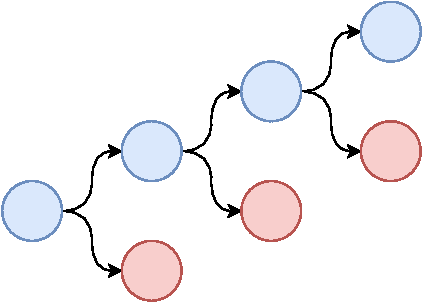
\includegraphics[scale = 0.8]{img/asim.pdf}
  \end{figure}
  \item \textbf{divisione simmetrica}, in cui le cellule staminali si dividono
  in due cellule staminali o in due cellule completamente differenziate:
  \begin{figure}[H]
    \centering
    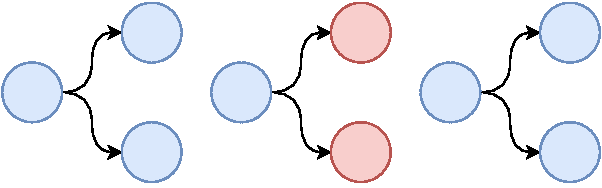
\includegraphics[scale = 0.8]{img/sim.pdf}
  \end{figure}
  \item \textbf{divisione ambientalmente asimmetrica}, anche se non è
  propriamente rappresentato, dove si può avere una divisione simmetrica o
  asimmetrica a seconda della presenza di un certo microambiente (con la
  conseguente presenza di determinate proteine) in cui si trova
  la cellula: 
  \begin{figure}[H]
    \centering
    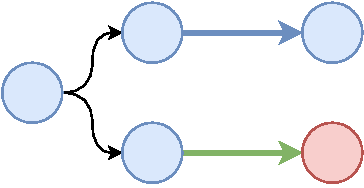
\includegraphics[scale = 0.8]{img/aasim.pdf}
  \end{figure}
\end{enumerate}
Si ha quindi che l'ambiente non è un aspetto trascurabile dal punto di vista
delle simulazioni. Nel ciclo cellulare, a seconda di quali sono gli insiemi di
proteine che vanno ad influire sul processo. Le cellule normalmente si trovano
in uno stato di \textbf{quiescenza}, normalmente indicato con $G_0$, mentre il
\textbf{ciclo cellulare} è il processo tramite il quale una cellula si
divide. L'ingresso nel ciclo cellulare è normalmente indicato con $G_1$ mentre
lo stato di esecuzione del processo con $G_2$, processo dove si ha anche uno
stato $S$ (\textit{non viene specificato altro a lezione}). Ci sono poi altri
stadi nel 
ciclo cellulare, tra cui lo stato di \textbf{mitosi}, solitamente indicato con
$M$, in cui si ha la divisione effettiva, che comporta due cellule che si
trovano in partenza nello stato $G_0$. Una cellula in stato $G_0$ può anche
\textit{morire in modo programmato}, tramite la cosiddetta
\textbf{apoptosi}. Tra lo stato $S$ e lo stato $G_2$ si ha che la presenza in
ambiente di determinate proteine può provocare le due possibili alternative
della \textit{divisione ambientalmente asimmetrica} in fase di
\textit{mitosi}, questo in quanto, nel momento in cui il DNA viene duplicato,
parti dello stesso vengono \textit{silenziate} mentre altre \textit{attivate} e
questa combinazione di eventi comporta la differenziazione delle due cellule
figlie.\\ 
Per modellare questo sistema usiamo un FSA, che poi potremmo codificare in un
qualsiasi linguaggio di programmazione, la semantica resta quella dell'FSA.\\
Vediamo quindi una versione semplificata di un FSA per questo modello. SI hanno
due sole variabili:
\begin{enumerate}
  \item $Ns$ che è il numero di cellule staminali
  \item $Np$ che è il numero di cellule progenitrici
\end{enumerate}
Si ha quindi:
\begin{figure}[H]
  \centering
  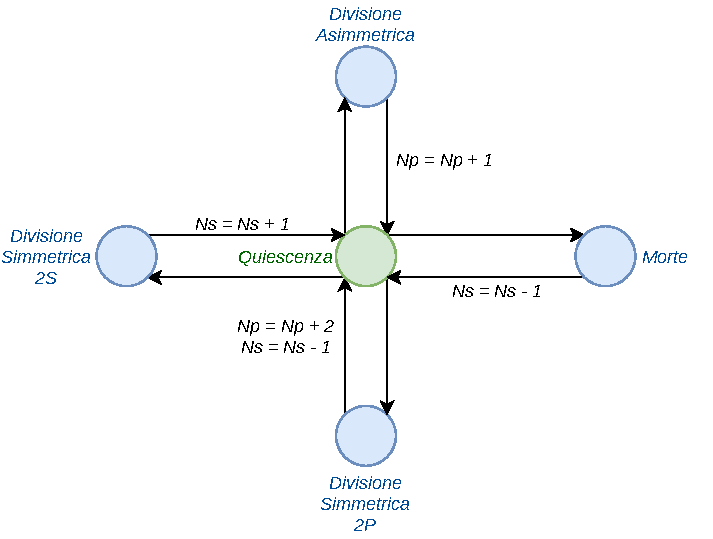
\includegraphics[scale = 1]{img/fsa1.pdf}
  \label{fig:fsa1}
\end{figure}
Dove si ha:
\begin{itemize}
  \item uno stato di \textit{quiescenza} dove si trovano le cellule
  \item quattro che rappresentano quattro differenti \textit{eventi} possibili,
  avendo che ogni evento comporta una certa modifica ad una o ad entrambe le
  variabili:
  \begin{itemize}
    \item divisione simmetrica di due cellule progenitrici, $2P$
    \item divisione simmetrica di due cellule staminali, $2S$
    \item divisione asimmetrica
    \item morte, nel dettaglio di una cellula staminale (volendo si potrebbe
    rappresentare anche lo stato di morte per una cellula progenitrice)
  \end{itemize}
\end{itemize}
% A questo sistema potremmo, volendo associare le seguenti EDO:
% \begin{gather*}
  
% \end{gather*}
In ogni caso quella data è quindi una \textbf{semantica}, per quanto
semplificata anche troppo (manca in primis una rappresentazione del tempo), di
un FSA per rappresentare modelli biologici. \\
Il \textbf{tempo} infatti è normalmente considerato associando un delay
esponenziale ad una transizione dell'FSA.\\
Si possono anche associare alle transizioni differenze probabilità per poter
passare ad uno stato partendo da un certo stato, ottenendo in pratica una
\textit{Markov chain}, ovvero un \textbf{sistema di transizione}. \\
Vediamo quindi come manipolare questi strumenti modellistici e cosa si ottiene
con il loro uso. Quello che viene prodotto è una \textbf{traccia}, ovvero una
\textit{sequenza ordinata} di vettori di valori, che volendo possono essere
\textit{simbolici}. Ad esempio, per l'FSA appena visto, potremmo avere come
traccia, dove ogni volta la coppia è formata dal numero di cellule staminali e
dal numero di cellule progenitrici: 
\[\langle{(100, 10^5),(101, 10^5)\ldots(98, 10^5)\rangle}\]
La nozione di \textit{traccia} ci permette di ragionare ad un ``livello più
basso'' e ci permette di definire sulla base delle tracce cos'è un
\textbf{Discrete Event Simulator (\textit{DES})}. Parlando dei DES si ha che la
semantica è più o meno la stessa però l'idea è che studiando come è fatta una
\textit{traccia} poi posso costruire un sistema che è di fatto più efficiente. I
DES sono molto utili anche per fare simulazioni iniziali di circuiti
elettronici. \\
L'architettura di un simulatore è formata da:
\begin{enumerate}
  \item una \textit{specifica di sistema} (che può essere, ad esempio, una
  rappresentazione tramite EDO)
  \item un \textit{engine} che, prese in input le specifiche di sistema, produce
  una \textit{traccia }di un sistema generando una serie di realizzazioni
  \item la \textit{traccia di simulazione} che raccoglie tutte le tracce
  prodotte dall'engine. Si ha una struttura interna
  \item una \textit{trace inspection} che manipola la traccia con un certo
  strumento, ad esempio, costruendo grafici, facendo analisi matematica,
  producendo una GUI etc$\ldots$ \\
  In alcuni casi si può anche interagire con la
  simulazione, interrompendola, ripetendo alcuni step, cambiare parametri ``a
  caldo'' etc$\ldots$ 
\end{enumerate}
Per implementare un simulatore banalmente si fa un \textit{loop}:
\begin{algorithm}[H]
  \begin{algorithmic}
    \For {$i$ \textbf{from} $start$ \textbf{to} $finish$}
    \State \textit{evaluate next ($i$)}
    \EndFor
  \end{algorithmic}
\end{algorithm}
dove \textit{evaluate next ($i$)} determina il tipo di simulazione che si sta
facendo.\\
\subsection{Simulatore di FSA}
Per implementare  un simulatore di FSA si ha:
\begin{itemize}
  \item come \textit{specifica} una rappresentazione di un FSA e si hanno quindi
  abbiamo alcune possibilità:
  \begin{itemize}
    \item costruire l'FSA e simularlo, tramite una funzione di transizione
    $\delta$, mettendo in conto che il consumo di 
    memoria cresce rapidamente (anche perché l'eventuale prodotto di un FSA con
    $N$ stati e di uno con $M$ stati produce in risultato $NM$ stati)
    \item tenere l'FSA separato e fare una simulazione più complessa
  \end{itemize}
  \item come \textit{engine} controllare l'insieme di tutte le transizioni
  abilitate dallo stato corrente e produrre lo stato successivo
\end{itemize}
Dal punto di vista ``programmativo'' si potrebbe usare anche solo una matrice.\\
La semantica di un DES è quindi quella di un FSA ma si ha una modalità di
esecuzione più efficiente dal punto di vista spaziale a patto di avere una coda
di eventi, per questo i DES sono scritti per tenere separati i diversi FSA. \\
Vediamo quindi come si implementa un DES. Si hanno:
\begin{itemize}
  \item come \textit{specifiche} si hanno sorgenti, ad esempio unità di
  computazione, come dei \textit{down samplers} (che riducono il campionamento
  del segnale) o delle operazioni logiche etc$\ldots$, che studiano, ad esempio,
  l'output di generatori di onde quadre 
  \item come \textit{engine} una \textit{coda con priorità} (per controllare
  quale evento far accadere prima) di coppie $\langle
  tempo, valore\rangle$, dove il valore può anche essere una struttura dati
  complessa. La coda contiene gli eventi che devono essere simulati. Si hanno
  poi i vari \textit{evaluators} delle unità, avendo che 
  ogni unità assume significato sse si hanno tutti i suoi input, potendo così
  produrre un output
\end{itemize}
Usando una coda di priorità, implementata tramite un \textit{heap}, abbiamo
tempi di inserimento e rimozione logaritmici (con un \textit{heap di Fibonacci}
si avrebbe addirittura inserimento in tempo costante). \\
Un esempio famoso è \textit{Simulink} che è il DES per \textit{MATLAB}.
\subsection{Simulatore di EDO}
Un esempio di simulatore che studia equazioni differenziali è il \textbf{metodo
  di Runge-Kutta al quart'ordine}, che appunto è un 
\textit{integratore} per EDO. È il metodo standard per integrare EDO ed è
abbastanza semplice da implementare.\\
Riprendendo la forma generale di una EDO, o di un sistema di EDO, si ha il
cosiddetto \textbf{problema del valore iniziale (\textit{initial-value
    problem})}, ovvero, avendo $t$ come 
variabile (che per noi tendenzialmente è il \textbf{tempo}) e $c$ come costante:
\[
  \begin{cases}
    \frac{\dd{y(t)}}{\dd{t}}=F(y(t),t)\\
    y(0)=c
  \end{cases}
\]
Si hanno quindi:
\begin{itemize}
  \item come \textit{specifica} un insieme di EDO
  \item come \textit{engine} si calcola in un numero discreto di passi il tempo
  il valore della funzione e della sua derivata. Come metodi numerici si hanno,
  ad esempio:
  \begin{itemize}
    \item il \textbf{metodo di Eulero}
    \item il \textbf{metodo di Runge-Kutta}, che può essere a diversi ordini,
    tipicamente al secondo o al quarto
    \item altri tipi di integratori, in particolare \textbf{metodi impliciti} in
    grado di trattare \textit{equazioni rigide}, \textit{vincoli algebrici},
    etc$\ldots$ 
  \end{itemize}
\end{itemize}
Non si ha quindi tendenzialmente uno studio analitico delle EDO, non essendo in
generale fattibile, ma si ha appunto uno studio numerico.
\subsubsection{Il metodo di Eulero}
Il \textbf{metodo di Eulero} non è più usato in quanto non ha caratteristiche
numeriche particolarmente ragionevoli, in primis perché ``accumula'' errori
molto velocemente. \\
SI usando degli indici per indicare il \textbf{passo i-esimo di computazione} e
si indica con $h$ il \textbf{passo di integrazione}, fisso.\\
Date queste premesse si supponga di avere l'n-esimo punto della funzione già
calcolato, ovvero $y_n$ si ha, per la forma di EDO indicata sopra:
\[y_{n+1}=y_n+h\cdot F(y_n,x_n)\]
In pratica l'idea generale dietro un integratore è quello di calcolare uno step
valutando la funzione $F$ allo step precedente e moltiplicando il risultato per
il passo di integrazione sommando per lo step precedente, ottenendo in pratica
la forma di una retta (tra il punto $x_n$ e il punto $x_{n+h}$).
\subsubsection{Il metodo di Runge-Kutta}
Il \textbf{metodo di Runge-Kutta al quart'ordine} supera il problema del
\textit{metodo di Eulero} di essere troppo lineare, dicendo che per vincolare
meglio il computo dei valori successivi della funzione $y$ è bene considerare
non solo il punto $x_{n+h}$ ma anche $x_{n+\frac{h}{2}}$. In particolare
``costringiamo'' la funzione a passare in un certo ``corridoio''.\\
Il \textit{metodo di Runge-Kutta al prim'ordine} è in pratica il \textit{metodo
  di Eulero} e si arriva a quanti ordini si vuole.\\ 
La formulazione completa di \textit{Runge-Kutta al quart'ordine} (quart'ordine
in quanto si calcolano quattro punti intermedi), detto anche
\textbf{metodo di Runge-Kutta 4} :
\begin{gather*}
  k_1=h\cdot F\left(x_n,y_n\right)\\
  k_2=h\cdot F\left(x_n+\frac{h}{2},y_n+\frac{k_1}{2}\right)\\
  k_3=h\cdot F\left(x_n+\frac{h}{2},y_n+\frac{k_2}{2}\right)\\
  k_4=h\cdot F\left(x_n+h,y_n+k_3\right)
\end{gather*}
Dove si nota che ogni $k_i$ è calcolato a partire da $F$ e da voli di $x_n$ e
$y_n$ che si conoscono e dai valori di $k_{i-1}$.\\
Si ha infine la formula per calcolare lo step successivo:
\[y_{n+1}=y_n+\frac{k_1}{6}+\frac{k_2}{3}+\frac{k_3}{3}+\frac{k_4}{6}+
  \mathcal{O}(h^5)\]
Introducendo quindi un errore è un $\mathcal{O}(h^5)$ (per questo viene anche
chiamato \textbf{metodo di Runge-Kutta 45}, indicando sia l'ordine, 4, che
l'ordine errore, 5), che è un valore molto
piccolo, fornendo un ottimo compromesso tra l'errore e la velocità di
computazione, ovvero la \textbf{velocità di convergenza} del metodo. \\
A livello computazionale serve quindi la funzione (passandola tendenzialmente
come \textit{funzione lambda}), il range, i valori iniziali etc$\ldots$ \\
Si ha che lo step $h$ può essere fisso o meno, avendo un \textbf{algoritmo
  adattivo}. 
\subsection{Sistemi Ibridi}
Ci si chiede cosa fare quando si ha una visione del sistema ``ad alto livello''
e una visione ``a basso livello'', avendo sistemi complessi che in uno stato si
comportano in un modo e in un altro stato in un altro, in uno stato magari si
usa un modello e in un altro un modello differente. Si mischiano quindi sistemi
con FSA, discreti, e sistemi con EDO, continui, creando dei \textbf{sistemi
  ibridi}. Un sistema ibrido può anche essere un sistema che in due stati
presenta due diversi insiemi di EDO, da scegliere in base a certe condizioni,
come ad esempio in figura \ref{fig:hyb}.\\
\begin{figure}
  \centering
  \begin{tikzpicture}[shorten >=1pt,node distance=4cm,on grid,auto]
    \node[elliptic state] (q_0) {$\frac{\dd{y}}{\dd{t}}=3$};
    \node[elliptic state] (q_1) [right=of q_0] {$\frac{\dd{y}}{\dd{t}}=-1.5$};
    \path[->]
    (q_0) edge [bend left = 25] node {$y>k_2$} (q_1)
    (q_1) edge [bend left = 25] node {$y<k_1$} (q_0);
  \end{tikzpicture}
  \caption{Esempio di sistema ibrido con due stati e le corrispondenti EDO,
    avendo che nel sistema vale $k_1>k_2$.}
  \label{fig:hyb}
\end{figure}
In un sistema ibrido con EDO cambia leggermente la forma del \textit{loop}
principale dell'integratore, avendo (con uno step fisso): 
\begin{algorithm}[H]
  \begin{algorithmic}
    \State $h\gets \langle\mbox{\textit{un certo valore}}\rangle$
    \For {$i$ \textbf{from} $start$ \textbf{to} $finish$}
    \State \textit{studia le EDO attuali ad uno step $h$}
    \If{\textit{si abilita una qualsiasi transizione}}
    \State \textit{cambia insieme di EDO}
    \EndIf
    \EndFor
  \end{algorithmic}
\end{algorithm}
Introducendo anche gli FSA in questo discorso potrei modellare, tramite un
\textit{sistema ibrido}, una popolazione di cellule staminali (e il conteggio
visto in figura \ref{fig:fsa1}) in modo più
realistico, più vicino alla natura discreta e stocastica del modello. Si
inserisce quindi un'equazione differenziale che modella il \textbf{tempo}, che
si evolve in modo costante, integrando:
\[\frac{\dd{time}}{\dd{t}}=1\]
Si associa quindi ad ogni transizione un ritardo esponenziale che rappresenta il
tasso di un evento del mio modello/popolazione (come la \textit{divisione
  asimmetrica} o l'\textit{apoptosi}).\\
Si ha quindi il seguente FSA:
\begin{figure}[H]
  \centering
  \begin{tikzpicture}[shorten >=1pt,node distance=9cm,on grid,auto]
    \node[elliptic state] (q_0) {$Morte/apoptosi$};
    \node[elliptic state,label={\small quiescenza}, align=center] (q_1)
    [right=of q_0] {$\frac{\dd{time}}{\dd{t}}=1$\\$r(morte)=random()$};
    \path[->]
    (q_0) edge [bend left = 25] node [above, align=center] {$test = \top $\\
      $Ns\gets Ns-1$\\ $Ns\gets Ns-1$} (q_1)
    (q_1) edge [bend left = 25] node [below]
    {$-\ln(r(morte))<\alpha\cdot Ns\cdot time$} (q_0);
  \end{tikzpicture}
  \label{fig:hyb2}
\end{figure}
Dove ad ogni integrazione in pratica ``tiro dei dadi'', avendo:
\begin{itemize}
  \item la transizione etichettata con un certo $test$, nel nostro caso:
  \[-\ln(r(morte))<\alpha\cdot Ns\cdot time\]
  scatta in base al ``lancio dei dadi'' fatto con $random()$
  \item la transizione che torna nello stato di quiescenza merita un
  approfondimento. 
  Avendo che se sono nello stato $morte/quiescenza$ test è sempre $\top$ e
  tornando nello stato $quiescenza$ si ``riazzera'' il tempo e si conteggia la
  ``morte'' di una cellula staminale
\end{itemize}
Ci sono dei problemi con gli algoritmi per la simulazione di \textit{sistemi
  ibridi}, specialmente \textit{problemi numerici}, ad esempio il problema del
\textbf{guard crossing}. Per questo problema si ha che, avendo ad esempio un
test del tipo $y(t)<0$, non seguendo la funzione  esattamente l'andamento
atteso, a livello numerico avendo l'integratore che integra solo in certi punti,
si rischia di ``perdere'' il test, non facendo il cambio di stato.\\
Si ha quindi un probelma di fedeltà rispetto a problemi che non si conosce
bene.
\chapter{Simulazionioni Stocastiche}
%$
Si introudcono ora le \textbf{simulazioni stocastiche}, ovvero ``l'altra faccia
della medaglia'' rispetto alle simulazioni discrete, sempre per reazioni
biochimiche. Si vedranno quindi varie rappresentazioni usabili per simulazioni
stocastiche e si vedrà un \textbf{metodo MonteCarlo}, ovvero il \textbf{metodo
  di Gillespie}, pensato appositamente per studiare reazioni chimiche e
biochimiche.\\
Il problema chiave quando si ragiona sulla simulazione di sistemi è che ci sono
differenze di evoluzione degli insiemi di reazioni biochimiche e biologiche che
può dipendere da un numero ``limitato'' di tipi di una certa molecola, ovvero al
dalla numerosità di una specie molecolare nel sistema. Dovendo considerare
questi effetti non si è più in grado di usare direttamente le EDO, in quanto
normalmente le EDO fanno vedere un ``comportamento aggregato'', ovvero un
\textit{comportamento medio}. Il comportamento che si vuole ora studiare invece
è un'approssimazione della risultante di molteplici comportamenti
individuali. Bisogna quindi capire come descrivere tali sistemi e un modo è
quello di usare la \textbf{Chemical Master Equation (\textit{CME})} che è una
rappresentazione precisa di questo comportamento, al costo di essere molto
``intrattabile'' dal punto di vista analitico (essendo quasi impossibile trovare
soluzioni chiuse di questa equazione, dovendo procedere a farne una simulazione
numerica). L'idea è quella quindi procedere numericamente ma procedendo in modo
da essere molto fedeli alla simulazione di una popolazione di individui.\\
In un modello deterministico, fissate le condizioni iniziali, il comportamento
complessivo del sistema è determinato. In un modello stocastico, date le stesse
condizioni iniziali, si possono avere comportamenti che sono qualitativamente
diversi e sono comportamenti che derivano da termini nel nostro modello che
rappresentano \textit{fluttuazioni casuali}. Si procede quindi, ad esempio,
introducendo del \textit{rumore} in una EDO, perdendo immediatamente la
possibilità di trovare soluzioni analitiche ma ottenendo un comportamento
comunque verosimile. L'introduzione di rumore normalmente non comporta un
cambiamento nella traiettoria complessiva del sistema ma a volte può accadere e
quello che si vuole garantire è che il modello permetta di riprodurre
comportamenti rilevabili anche in un normale esperimento di laboratorio.
\section{Modelli di Markov}
Il modo più semplice per rappresentare questo tipo di modelli è comunque quello
di usare un \textbf{processo di Markov}, che siano \textbf{catene di Markov} o
\textbf{sistemi di transizione}.\\
Preso un processo di Markov si possono aggiungere ulteriori vincoli sullo scatto
di una transizione, associando \textit{condizioni} e/o \textit{azioni} agli
archi, in modo tale che un sistema passi da uno statoi all'altro sse una
condizione è vera e facendo scattare una certa serie di azioni che modificano lo
stato del sistema. Tutto questo fa giustificato dal punto di vista
matematico. \\
Una cosa che si fa con le \textbf{catene di Markov} è quello di studiare il
comportamento nel lungo periodo, studiando il cosiddetto \textbf{steady state
  (\textit{stato stazionario})}. Data la matrice di transizione $P$ e il vettore
di stato $v$ che rappresenta una distribuzione di probabilità (sommando 1) sugli
stati, possiamo definire le varie proprietà (\textbf{\textit{guardare appunti di
    Modelli Probabilistici per le Decisioni}}). \\
Si possono anche definire varie estensioni, tra cui:
\begin{itemize}
  \item Semi-Markov processes
  \item Generalized Semi-Markov processes
  \item Reti di Petri stocastiche
  \item $\ldots$
\end{itemize}
Torniamo alle definizioni di base ricordiamo che un \textbf{vettore di
  probabilità} ha tutte entry non negative che sommano a 1, avendo che ogni
entry rappresenta una certa probabilità associata ad un dato stato. Solitamente
si parte da un vettore $v_0$ che rappresenta la distribuzione iniziale di
probabilità e si ha che $v=v_{0}\cdot P$, se si fa un singolo
step. Se volessi ottenere la distribuzione dopo $n$ passi (avendo passi
discreti) avrei $v_ni=v_{0}\cdot P^n$. Se si ha che $v\cdot P = v$ ho che $v$ è
un \textit{vettore di steady state}, essendo in uno \textbf{stato
  stazionario}. Lo \textit{stato stazionario} si noti essere un
\textit{autovettore} della matrice $P$.
\newpage
\section{Reti di Petri}
Passiamo ora alle \textbf{reti di Petri}.\\
Le \textit{reti di Petri}, specialmente quelle \textit{stocastiche}, sono un
interessante formalismo che si può usare per rappresentare le interazioni (di
tipo biochimico etc$\ldots$) tra varie \textit{entità biologiche}. Le
\textit{reti di Petri} hanno infatti trovato in primis uso nella
rappresentazione di reazioni chimiche.\\
In figura \ref{fig:pet1} troviamo un semplice esempio dove si rappresenta
sostanzialmente il processo di traduzione e trascrizione di una proteina. Se
abbiamo un \textit{gene inattivo}, che può diventare un \textit{gene
  attivo}. Quando attivo il gene può sia produrre una proteina che rimanere
attivo, fino a quando non torna ad essere inattivo. Le varie lettere greche
associate alle varie transizioni hanno una precisa interpretazione e sono il
\textbf{tasso di attivazione} di ognuna delle transizioni, ovvero si associa un
ritardo, distribuito di fatto in modo esponenziale, ad ogni transizione,
aggiungendo un tempo esterno al sistema e ottenendo una \textbf{rete di Petri
  stocastica}. 
\begin{figure}
  \centering
  \begin{tikzpicture}[node distance=2cm,bend angle=45,auto]
    \node [place, label = above: $inactive\,\,\,gene$, tokens = 1] (p0)  {};    
    \node [transition] (t1) [below right of = p0, label = right: $\lambda$] {};
    \node [transition] (t2) [below left of = p0, label =  left: $\mu$] {};
    \node [place] (p1)  [below right of = t2, label = below:
        $active\,\,\,gene$]  {}; 
    \node [transitionv] (t3) [right of = p1, label = above: $\nu$] {};
    \node [place] (p2) [right of = t3, label = above: $protein$] {};
    \node [transitionv] (t4) [right of = p2, label = above: $\delta$] {};
    \node [] (p3) [right of = t4] {$\ldots$};
    \path[-{Latex[width=2mm]}]
    (t2) edge (p0)
    (p0) edge (t1)
    (t1) edge (p1)
    (p1) edge (t2)
    (p1) edge [bend left = 25] (t3)
    (t3) edge [bend left = 25] (p1)
    (t3) edge (p2)
    (p2) edge (t4)
    (t4) edge (p3)
    ;
  \end{tikzpicture}
  \caption{Esempio di porzione di rete di petri stocastica}
  \label{fig:pet1}
\end{figure}
Le \textit{reti di Petri}, intese come \textit{sistemi elementari} o
\textit{reti P/T}, sono solo una delle estensioni delle
\textit{reti di Petri} utili. Una delle principali limitazioni è quella
dell'assenza della rappresentazione del tempo. Tra le estensioni più usate se ne
menzionano due, 
in grado di aggiungere informazioni alle \textit{catene di Markov}, perlomeno
dal punto di vista del formalismo grafico:
\begin{enumerate}
  \item \textbf{reti di Petri temporizzate}
  \item \textbf{reti di Petri stocastiche}, già citate
\end{enumerate}
\subsection{Reti di Petri Temporizzate}
Le \textbf{reti di Petri stocastiche} permettono di avere l'informazione
temporale associata ad ogni singolo elemento della rete:
\begin{itemize}
  \item \textit{posti}
  \item \textit{transizioni}, che è il caso più comune
  \item \textit{archi}
  \item \textit{marche}
  \item $\ldots$
\end{itemize}
Vediamo il caso più comune.\\
Tipicamente ogni transizione $t$ ha un valore di ritardo, ovvero un intervallo
di tempo nel quale può attivarsi dal momento in cui diventa abilitata. Tale
valore è rappresentato dalla coppia $[d,D]$, dove $d$ è il minimo quantitativo
di unità temporali per l'esecuzione mentre $D$ il massimo.\\
Uno degli utilizzi di tali reti è quello di misurare le prestazioni ma hanno una
forte limitazione d'uso in presenza di \textbf{conflitti} nella rete.\\
Quando si hanno diverse transizioni che sono contemporaneamente abilitate si
sceglie quella che deve avvenire prima, ovvero quella con la \textit{scadenza
  più vicina}. In ogni momento ho quindi una priorità su quale transizione far
scattare. Potrei comunque avere più transizioni abilitate con la medesima
scadenza e questo è un problema, dovendo fare un'ulteriore scelta, magari
facendole scattare tutte (per questo il discorso legato ai \textit{conflitti})
oppure scegliendone un sottoinsieme in modo arbitrario.
\subsection{Reti di Petri Stocastiche}
Con le \textbf{reti di Petri stocastiche} quello che succede è che si associa ad
ogni transizione un \textit{ritardo/delay} normalmente distribuito con un tasso
di ritardo costante $\lambda_T$.\\
Si ha quindi che, indicando con $P(x)$ la probabilità che avvenga un evento $x$,
che la probabilità che una certa transizione accada esattamente al tempo $\tau$:
\[P(X_T=\tau)=\lambda_Te^{-\lambda_T\tau}\]
e che la stessa transizione accada prima di un certo tempo:
\[P(X_T\leq\tau)=1-\lambda_Te^{-\lambda_T\tau}\]
Avendo un ritardo medio pari a $\frac{1}{\lambda}$.\\
Il valore di ritardo/delay associato alla transizione $T$ è appunto $X_T$ che è
una variabile casuale e la sua funzione di densità di probabilità è distribuita
in modo esponenziale sul parametro $\lambda$. Come conseguenza si ha che la
probabilità che due transizioni siano abilitate contemporaneamente è
estremamente bassa, praticamente nulla. Di fatto quindi possiamo osservare che
per costruzione il sistema si comporta come se ci fosse una singola transizione
abilitata in ogni istante, risolvendo il problema riscontrato con le
\textit{reti di Petri Temporizzate}.\\
Vediamo un ulteriore semplice esempio.\\
Si hanno due transizioni, $t_1$ e $t_2$, con associati i rispettivi $\lambda_1$
e $\lambda_2$. 
\begin{figure}[H]
  \centering
  \begin{tikzpicture}[node distance=2cm,bend angle=45,auto]
    \node [place, tokens = 1] (p0)  {};
    \node [place, right of = p0, tokens = 1] (p1)  {};
    \node [place, right of = p1, tokens = 1] (p2)  {};   
    \node [transition] (t1) [below left of = p1, label = left: $\lambda_1$] {};
    \node [transition] (t2) [below right of = p1, label =  right: $\lambda_2$]
    {}; 
    \node [place, below of = t1] (p3)  {};
    \node [place, below of = t2] (p4)  {}; 
    \path[-{Latex[width=2mm]}]
    (p0) edge (t1)
    (p1) edge (t1)
    (p1) edge (t2)
    (p2) edge (t2)
    (t1) edge (p3)
    (t2) edge (p4)
    ;
  \end{tikzpicture}
\end{figure}
Entrambe le transizioni sono abilitate nello stato iniziale e bisogna capire chi
scatta per prima. Inoltre lo scatto di una delle transizioni disabilita l'altra,
avendo appunto un \textit{conflitto}. In realtà in questo caso, essendo entrambe
le transizioni abilitate, si assegnano alle due transizioni due nuovi tassi:
\[\lambda_1'=\frac{\lambda_1}{\lambda_1+\lambda_2}\]
\[\lambda_2'=\frac{\lambda_2}{\lambda_1+\lambda_2}\]
Poi si calcolerà cosa accade dopo lo scatto di una delle due. \\
Con queste reti si ha un equivalente delle \textbf{catene di Markov a tempo
  continuo}, grazie al fatto che il rateo è esponenziale e che le reti sono
\textit{senza memoria}.\\
(\textbf{\textit{Parte non capita a fondo}}).\\
Avendo quindi l'approssimazione che si ha una sola transizione abilitata in
ogni istante quello che si può dire è che la semantica delle \textbf{reti di
  Petri stocastiche} è la stessa delle \textbf{catene di Markov} ma si ha, con
le reti, un vantaggio dal punto di vista della mera rappresentazione grafica,
avendo una rappresentazione molto concisa rispetto a quella delle catene,
permettendo di dare più informazione in ``meno spazio''. Con le \textit{reti di
  Petri stocastiche} si perde però un pezzo di espressività rispetto a quelle
standard, in quanto, introducendo i vincoli di rateo, si riduce la rete ad un
FSM a cui sono aggiunte le probabilità, anche se le FSM avrebbero meno
espressività. Le reti di Petri generano linguaggi che non sono
\textit{context-free} ma ci sono linguaggi \textit{context-free} che non possono
essere generati dalle reti. In ogni caso l'insieme dei linguaggi
generati/riconosciuti contiene propriamente quello relativo alle FSM. \\
L'analisi quantitativa di tali reti è comunque permessa solo se si ha conoscenza
dei ratei di ritardo delle varie transizioni e questo permette l'uso delle
stesse per valutare prestazioni.\\
Ci sono molte estensioni relative alle \textit{reti di Petri stocastiche} e si
hanno vari pacchetti standard per le simulazioni.\\
Vediamo ora il rapporto tra le reti e le applicazioni
biologiche\footnote{Quantitative Modeling of Stochastic Systems in
  Molecular Biology using Stochastic Petri Nets, Peter J.E. Goss and Jean
  Peccoud, PNAS, 95, 6750-6755, June 1988} in questa tabella riassuntiva delle
relazioni tra gli elementi della rete e la biologia:
\begin{table}[H]
  \centering
  \begin{tabular}{c|c}
    \textbf{Elemento della rete} & \textbf{Corrispettivo biologico}\\
    \hline
    \hline
    posti & specie molecolari\\
    \hline
    marca & molecola\\
    \hline
    numero di marche & numero di molecole\\
    \hline
    transizioni & reazioni\\
    \hline
    posto di input & reagente\\
    \hline
    posto di output & prodotto\\
    \hline
    funzione di peso & tasso della reazione\\
    \hline
    transizione abilitata & reazione possibile\\
    \hline
    scatto & avvenimento della reazione
  \end{tabular}
\end{table}
Questo è quindi \textbf{un modo} per rappresentare sistemi biologici, tramite
\textit{reti di Petri stocastiche}, quindi con la semantica delle \textit{catene
  di Markov}.
\section{Algoritmi di Gillespie}
Passiamo quindi a studiare le \textit{simulazioni stocastiche}, ovvero, data una
rappresentazione delle reazioni in un sistema discreto e stocastico, effettuare
la simulazione ottenendo risultati ragionevoli, nel dettaglio tramite i
cosiddetti \textbf{algoritmi di Gillespie}.\\ 
Si hanno alcuni aspetti biologici da considerare:
\begin{itemize}
  \item molti processi biologici coinvolgono un numero basso di molecole
  \item trascrizione e traduzione hanno un comportamento stocastico
\end{itemize}
Spesso quindi si hanno fenomeni davvero molto complessi e quindi si ``ripiega''
verso una simulazione stocastica e non esatta.\\
Ci sono molti modelli scaricabili dai già citati database, come
\textit{BioModels, Reactome, KEGG $\ldots$} e molti di questi modelli sono
\textbf{pathway}, ovvero, si ricorda, collezioni di reazioni connesse tra loro
organizzate in una rete, che spesso è un grafo completamente connesso. \\
(\textbf{Su Moodle due esempi di pathway, quello di $Wnt$, una proteina molto
  importante, e quello di $TGF\mbox{-}\beta$, importante nello studio del
  \textit{colon}}).\\ 
Possiamo usare vari modi per costruire tali modello di pathway, che siano
\textit{reti di Petri} ma anche linguaggi e sistemi \textit{rules-based}, come
\textit{Bionetgen}. In entrambi i casi si ottiene un formalismo per
rappresentare un sistema che poi viene simulato tramite algoritmi di
Gillespie. Tali algoritmi sono algoritmi di simulazione stocastica della classe
degli \textbf{algoritmi/metodi Montecarlo} che hanno la peculiarità di essere
molto semplici da implementare e sono molto utili permettendo di considerare
comportamenti dove gli effetti di alcune, poche, molecole possono influire su
tutto il sistema. Questi algoritmi sono giustificati in modo molto rigoroso dal
punto di vista fisico (da notare che il primo fu pubblicato nel 1974 su
\textit{Journal of computational physics} e anche i successivi articoli sono
sempre legati a riviste legate al mondo della fisica, come ad esempio
\textit{Journal of Chemical Physics}). Questi studi sono stati poco considerati
fino agli anni 2000 e poi sono ``esplosi'' dal punto di vista delle citazioni.\\
Vediamo quindi il funzionamento di tali algoritmi.\\
Si parte dal descrivere lo \textit{stato dinamico del sistema} che è dato da un
vettore numerico $\mathbf{X}(t)$, non negativo, dove ogni elemento $X_i(t)$
rappresenta esattamente il numero di molecole che si hanno della specie $S_i$ al
tempo $t$: 
\[\mathbf{X}(t)=[X_1(t),\ldots, X_N(t)]\]
Questo vettore è direttamente rappresentabile come un vettore di marcatura nelle
\textit{reti di Petri}.\\
L'obiettivo è quindi studiare l'evoluzione di $\mathbf{X}(t)$ a partire da un
certo stato iniziale $\mathbf{X}(0)=\mathbf{x}_0$.\\
Ogni reazione $R_j$ è caratterizzata da due oggetti matematici:
\begin{enumerate}
  \item il \textbf{vettore di cambio di stato (\textit{state change vector})}:
  \[\beta_j=\left(\beta_{1j}, \ldots, \beta_{nj}\right)\]
  che nelle \textit{reti di Petri} è il \textit{vettore di scatto}. Si ha quindi
  che $\beta_{kj}$ è il cambio di popolazione della specie molecolare $S_k$ dopo
  un'occorrenza della reazione $R_j$. Quindi se il sistema è nello stato
  $\mathbf{x}$ e $R_j$ occorre allora lo stato del sistema passa a
  $\mathbf{x}+B_j$.\\ 
  La matrice $[\beta_{ij}]$, data da specie/reazione (specie sulle righe e
  reazioni sulle colonne), è detta \textbf{matrice stochiometrica}, che quindi
  rappresenta i possibili cambiamenti di stato dell'intero sistema date tutte le
  reazioni
  \item la \textbf{funzione di propensità} $a_j$. Si ha che $a_j(x) \dd{t}$ è la
  probabilità che, dato $X(t)=\mathbf{x}$, un'occorrenza di $R_j$ accadrà
  all'interno del \textbf{volume} $V$ (dato che si assume che le reazioni
  avvengano in un certo volume ben definito) in un prossimo intervallo
  infinitesimale di tempo lungo $\dd{t}$, quindi in $[t,t+\dd{t}]$. Questa
  funzione quindi dipende dallo stato attuale
\end{enumerate}
\begin{esempio}
  Vediamo un quindi un piccolo esempio:
  \begin{figure}[H]
  \centering
  \begin{tikzpicture}[node distance=2cm,bend angle=45,auto]
    \node [place, tokens = 1, label = above: $S_2$] (p0)  {};
    \node [transition] (t1) [below of = p0, label = below: $R_1$] {};
    \node [place, left of = t1, tokens = 1, label = above: $S_1$] (p1)  {};
    \node [transition] (t2) [below of = t1, label =  below: $R_3$] {};
    \node [place, right of = t1, tokens = 1, label = above: $S_3$] (p2)  {};
    \node [transition] (t3) [right of = p2, label =  below: $R_2$] {};
    \node [place, right of = t3, tokens = 1,  label = above: $S_5$] (p3) {};    
    \path[-{Latex[width=2mm]}]
    (p0) edge (t1)
    (p1) edge (t1)
    (t1) edge (p2)
    (p2) edge (t3)
    (t3) edge (p3)
    (t2) edge [bend left = 45]  (p0)
    (t3) edge (p0)
    (p2) edge   (t2)
    (t2) edge [bend left = 25]   (p1)
    ;
  \end{tikzpicture}
\end{figure}
E ci chiediamo quanto vale il cambiamento di stato nel caso scatti $R_2$ (che
scatta sse $S_3>0$):
\[\beta_2=\left(\beta_{12}, \beta_{22},\beta_{32},\beta_{42}\right)\]
Si ha quindi banalmente che:
\[\beta_2=(0,1,-1,1)\]
Avendo che la specie $S_1$ non viene toccato, alle specie $S_2$ e $S_4$ si
aggiunge una marca mentre alla specie $S_3$ ne viene tolta una.
\end{esempio}
\begin{esempio}
  Vediamo un altro esempio.\\
  Si ha una reazione $R_1$ data da:
  \[[X_1]+[X_2]\to 2[X_3]\]
  Si ha quindi:
  \[a_1(\mathbf{x})=c_1x_1x_2\]
  con:
  \begin{itemize}
    \item $x_1=\mathbf{x}(1)$
    \item $x_2=\mathbf{x}(2)$
    \item $c_1$ costante correlata alla reazione quando si fa il trattamento
    della stessa nel caso deterministico, ovvero quando si considera, ad esempio
    la \textit{legge di massa/azione}. Tale costante è quindi legata al rateo
    costante $k_1$ in questo modo:
    \[c_1=\frac{k_1}{V}\]
  \end{itemize}
  Si ha comunque un certo insieme di valori per $\beta_1$.\\
  Data questa forma di rappresentazione delle reazioni calcolo direttamente sia
  l'equazione differenziale ma anche la \textbf{funzione di propensità} (che ha
  una derivazione simile per quanto ci sia una forte differenza concettuale
  essendo una probabilità).\\
  \emph{La forma della \textbf{funzione di propensità} segue direttamente dalla
    fisica molecolare e dalla teoria cinetica delle reazioni.}
\end{esempio}
\subsection{Chemical Master Equation}
Uno dei problemi principali in fase di simulazione è che non si conosce la
precisa posizione e la precisa velocità delle varie molecole nel volume $V$
(\textit{si pensi alla teoria molecolare dei gas}). Si procede quindi predicendo
la probabilità che una reazione accada nel tempo successivo $\dd{t}$ e
predicendo che questa reazione sia $R_j$, parlando di \textit{dinamica
  probabilistica}. \\ 
Ogni reazione è caratterizzata dal \textit{vettore di cambio di stato} e
dalla \textit{funzione di propensità} e siamo in grado di calcolare la
probabilità che $R_j$ accada nel prossimo intervallo di tempo di ampiezza
$\dd{t}$. Possiamo quindi calcolare la probabilità a partire da uno stato
iniziale e ad un tempo iniziale:
\[P(\mathbf{x},t|\mathbf{x}_0,t_0)\]
che è appunto la probabilità di avere il vettore di stato $\mathbf{x}$ per la
popolazione al tempo $t$ dati uno stato di partenza $\mathbf{x}_0$ e un tempo di
partenza $t_0$. Questa probabilità, una volta ben scritta, viene chiamata
\textbf{chemical master equation}.\\
Per studiare meglio tale equazione consideriamo anche un'altra probabilità:
\[P(\mathbf{x},t+\dd{t}|\mathbf{x}_0,t_0)\]
dove si è aggiunto il ``passo temporale'' $\dd{t}$. Dobbiamo capire come
trovarci allo stato $\mathbf{x}$ al tempo $t+\dd{t}$. Uno dei modi è pensare di
trovarsi al tempo $t$ nello stato $\mathbf{x}$ e non avere alcune reazione per
un tempo $\dd{t}$, in modo da essere ancora in $\mathbf{x}$ al tempo
$t+\dd{t}$. In pratica mi serve la seguente probabilità congiunta:
\[P(\mathbf{x},t+\dd{t}|\mathbf{x}_0,t_0)=P(\mathbf{x},t|\mathbf{x}_0,t_0)\cdot
  \left(1-\sum_{j=1}^Ma_j(\mathbf{x})\dd{t}\right)\]
Dove $1-\sum_{j=1}^Ma_j(\mathbf{x})\dd{t}$ rappresenta la probabilità che non
accada alcuna reazione (essendo uno meno la probabilità che una qualsiasi
reazione accada).\\
Ovviamente questo non è l'unico modo, infatti potrebbe succedere che occorra una
reazione $j$ nell'intervallo di tempo lungo $\dd{t}$. Questo però può succedere
sse la reazione $j$-esima è accaduta nell'intervallo di tempo $\dd{t}$ e il
sistema si trovava nello stato $\mathbf{x}-\beta_j$, ovvero nello stato
antecedente all'occorrenza della reazione. In tal caso si ha quindi:
\[P(\mathbf{x},t+\dd{t}|\mathbf{x}_0,t_0)=P(\mathbf{x}-\beta_j,t|
  \mathbf{x}_0,t_0)\cdot a_j(\mathbf{x}-\beta_j)\dd{t}\]
Ovviamente si9 hanno $M$ possibili reazione e quindi bisogna sommare tutti i
$j$-esimi termini ottenuti con questa formula (anche se normalmente si ha
l'occorrenza di una sola reazione). \\
Avendo quindi visto i due possibili casi possiamo ottenere la formula finale per
la \textbf{chemical master equation}.\\
Definiamo prima la la somma tra la
probabilità che nell'intervallo di tempo $\dd{t}$, partendo dal tempo $t$ non
avvenga alcuna reazione e quella che avvengano un certo numero $M$ di
reazioni: 
\begin{align*}
  P(\mathbf{x},t+\dd{t}|\mathbf{x}_0,t_0)=&P(\mathbf{x},t|\mathbf{x}_0,t_0)
                                            \cdot
                                            \left(1-\sum_{j=1}^Ma_j(\mathbf{x})\dd{t}\right)\\
  +& \sum_{j=1}^M(P(\mathbf{x}-\beta_j,t|
     \mathbf{x}_0,t_0)\cdot a_j(\mathbf{x}-\beta_j)\dd{t})
\end{align*}
Pur ricordando, per la seconda sommatoria, che raramente accadono più di una
reazione.\\
Studiamo un po' la formula appena ottenuta. Se sottraiamo da entrambe le parti
$P(\mathbf{x},t|\mathbf{x}_0,t_0)$, dividiamo per $\dd{t}$ e ne calcoliamo il
limite che tende a 0 otteniamo:
{\small{\[\frac{\partial
    P(\mathbf{x},t+\dd{t}|\mathbf{x}_0,t_0)}{\partial t}=\sum_{j=1}^M\left(
 a_j(\mathbf{x}-\beta_j)\cdot
 P(\mathbf{x}-\beta_j,t|\mathbf{x}_0,t_0)-a_j(\mathbf{x})\cdot P(\mathbf{x},t|
 \mathbf{x}_0,t_0)\right)\]}}
Ovvero ottengo la variazione della probabilità nell'intervallo di tempo
$\dd{t}$, che è la vera e propria \textbf{Chemical Master Equation
  (\textit{CME})}.  \\
Si noti che la \textit{CME} è un'\textbf{equazione differenziale stocastica} che
è intrattabile, se non in casi molto semplici, dal punto di vista analitico. Un
pathway non rientra nella casistica dei casi semplici, avendo un elevato numero
di specie solitamente rappresentate. L'equazione, per quanto intrattabile, ci
dice comunque come poter costruire un sistema che ci permetta di simularla,
simulando l'evoluzione nel tempo del sistema.\\
\textbf{Gillespie dimostrò che si può derivare la \textit{CME} dal suo algoritmo
  di simulazione (\textit{forse anche viceversa}).}
\subsection{Implementazione degli Algoritmi di Gillespie}
Vediamo quindi come implementare un sistema di simulazione stocastica che ci
permetta di seguire l'evoluzione di un insieme di reazioni nel tempo.\\
Dato che la \textit{CME} è intrattabile generiamo \textbf{traiettorie} di
$\mathbf{X}(t)$ da studiare. Ovviamente non sono tutte le possibili traiettorie
ma se ne generano abbastanza per poter fare, \textit{ex-post}, uno studio
statistico su queste traiettorie. Questo non è uguale a fare uno studio numerico
della \textit{CME} in quanto si costruisce un algoritmo che ogni volta genera
una certa traiettoria, ripetendo più volte la simulazione e osservando infine un
insieme di realizzazioni che sono consistenti con la \textit{CME}.\\
Comunque ci serve un algoritmo numerico e questo è appunto l'\textbf{algoritmo
  di Gillespie}.\\
Tale algoritmo prevede alcune assunzioni:
\begin{itemize}
  \item un volume fissato $V$ a temperatura costante
  \item un numero $N$, $N>1$, di specie molecolari in una miscela ben mischiata
  che interagiscono chimicamente nel volume $V$: $S_1,S_2,\ldots,S_N$ 
  \item un numero $M$, $M>1$, di possibili reazioni: $R_1,R_2,\ldots,R_M$
  \item ci sia equilibrio termico ma non equilibrio chimico (avendo appunto che
  alcune reazioni possono accadere)
\end{itemize}
L'assunzione di miscela ben mischiata è un'assunzione essenziale per avere una
buona simulazione. Il citoplasma non è una miscela ben mischiata, portando
quindi a ``prendere con le pinze'' le simulazioni. \\
Per vedere come funziona l'algoritmo, di per sé molto banale, bisogna capire la
matematica che c'è dietro. \\
IL primo punto chiave è la seguente probabilità, dato
$\mathbf{X}(t)=\mathbf{x}$, con $j$ indice della prossima reazione e $\tau$
tempo della prossima reazione: 
\[P(\tau, j|\mathbf{x},t)\]
ovvero la probabilità che la reazione $j$-esima, ovvero $R_j$, accada
nell'intervallo di tempo infinitesimale $[t+\tau, t+\tau+\dd{t}]$. Questa è in
pratica la probabilità che voglio calcolare e si nota che non è la stessa della
\textit{CME} ma è la \textbf{la funzione di densità di probabilità congiunta
  condizionata di due variabili casuali $j$ e $\tau$}.\\ 
Considero ora la probabilità:
\[P_0(\tau|\mathbf{x},t)\]
ovvero la probabilità che
non accada alcuna reazione nell'intervallo $[t,t+\tau]$, dato lo stato
$\mathbf{X}(t)=\mathbf{x}$ (si nota come si stia ragionando come nel caso della
\textit{CME}). Ne segue, facendo derivazioni simile a quelle fatte per la
\textit{CME}, che: 
\[P(\tau,j|\mathbf{x},t)\dd{t}=P_0(\tau|\mathbf{x},t)\cdot
  a_j(\mathbf{x})\dd{t}\]
Si ha anche qui la probabilità accada una qualche reazione, avendo in tal caso:
\[P_0(\tau+\dd{t}|\mathbf{x},t)=P_0(\tau|\mathbf{x},t)\cdot\left(1-sum_{j=1}^M
    a_j(\mathbf{x})\dd{\tau}\right)\]
Prendendo infine il limite per $\dd{\tau}$ che tende a 0 e risolvendo
l'equazione differenziale per ottenere una soluzione analitica, si ottiene:
\begin{gather*} 
  P_0(\tau|\mathbf{x},t)=e^{-a_0(\mathbf{x})\tau}\\
  a_0(\mathbf{x})\equiv \sum_{j=1}^M a_j(\mathbf{x})
\end{gather*}
Ma a questo punto, ricordando che:
\[P(\tau,j|\mathbf{x},t)\dd{t}=P_0(\tau|\mathbf{x},t)\cdot
  a_j(\mathbf{x})\dd{t}\]
si ottiene che:
\[P(\tau,j|\mathbf{x},t)=a_j(\mathbf{x})\cdot e^{-a_0(\mathbf{x})\tau}\]
Data quest'ultima equazione si può andare a calcolare effettivamente il $\tau$
e il $j$ che serve semplicemente usando una generazione di numeri
pseudo-casuali. Si usa una distribuzione uniforme per generare due numeri, $r_1$
e $r_2$ in $[0,1]$ e a quel punto si ha che:
\[\tau=\frac{1}{a_0(\mathbf{x})}\ln\left(\frac{1}{r_1}\right)\]
mentre $j$ è il più piccolo intero tale che sia soddisfatta la seguente
condizione: 
\[\left(\sum_{i=1}^ja_i(\mathbf{x})\right)>r_2a_0(\mathbf{x})\]
Ho quindi stabilito in modo causale quando accadrà la prossima reazione e quale
sarà questa reazione. \\
Possiamo quindi definire i vari passi dell'\textbf{algoritmo di Gillespie}:
\begin{enumerate}
  \item si inizializzano $t=t_0$ e $\mathbf{x}=\mathbf{x}_0$
  \item a partire dallo stato $\mathbf{x}$ al tempo $t$ si calcolano tutte le
  $a_j(\mathbf{x})$ (quindi per ogni reazione) e quindi posso calcolare
  $a_0(\mathbf{x})$. Questo è un passaggio costoso dal punto di vista
  computazionale 
  \item si generano pseudo-casualmente $\tau$ e $j$, come visto precedentemente
  (e la generazione di $r_1$ e $r_2$ è la cosa computazionalmente più costosa
  qui) 
  \item si aggiorna $\mathbf{x}$ a $\mathbf{x}+\beta_j$ (simulando l'occorrenza
  della reazione) e si aggiorna $t$ a $t+\tau$
  \item si salva la coppia $(\mathbf{x}, t)$ e si torna al passaggio 2.
  Alternativamente è possibile concludere la simulazione (in base al fatto che
  si ha computato per troppo tempo o che magari il sistema non cambia da
  parecchie iterazioni)
\end{enumerate}
Il ciclo centrale dell'algoritmo è quindi molto semplice \textit{(nel secondo
  paper di Gillespie c'è il codice in \emph{Fortran}}), al più di sapere come
funzioni la matematica sottostante e conoscere la rappresentazione interna
delle reazioni, dei cambiamenti di stato etc$\ldots$\\
L'\textit{algoritmo di Gillespie} è definibile \textbf{esatto} in quanto
le sue realizzazioni sono in accordo con la \textit{CME}. Si osserva inoltre che
le proprietà statistiche di un insieme di traiettorie generate dall'algoritmo,
in linea di principio, danno un'informazione accurata circa il comportamento
stocastico globale di un sistema dinamico come previsto dalla \textit{CME}.\\
L'\textit{algoritmo di Gillespie} è computazionalmente costoso, dal punto di
vista temporale più che spaziale. Potremmo avere un sistema con reazioni molto
probabili su cui ``oscilla'' il sistema per molto tempo, prima che la
generazione pseudo-casuale renda possibile un'altra reazione. Un altro problema
è che $a_0(\mathbf{x})$ può essere molto grande in presenza di un gran numero di
molecole della stessa specie e questo rende $\tau$ (essendo $a_0(\mathbf{x})$ a
denominatore nella formula) molto piccolo, rallentando molto la
simulazione. Quest'ultimo aspetto si contrappone a quanto accade in un
simulatore deterministico dove, ad esempio, si ha un passo di integrazione fisso
su cui si ha un certo controllo e che garantisce che la simulazione avanza in
modo controllato mentre qui non si ha questo aspetto.\\
L'\textit{algoritmo di Gillespie} è quindi molto semplice da implementare anche
se molto costoso dal punto di vista delle risorse. Si ha inoltre che avendo
molte reazioni e molte specie hanno conseguenze sul ciclo e, ad esempio, se una
reazione coinvolge pochissime molecole questa viene ``ignorata'' a favore di
reazioni che coinvolgono molte molecole. Bisogna quindi fare molte simulazioni
(cambiando il \textit{seed} del generatore pseudo-causale) per capire come
funzioni verosimilmente il sistema e caratterizzarlo al meglio. Questa cosa
comporta anche molta interazione ``manuale'' nonché ulteriori costi
computazionali.\\
L'\textit{algoritmo di Gillespie} è molto usato in biologia computazionale, ad
esempio in simulatori come \textit{COPASI, StochSim etc$\ldots$}
\subsection{Variante Tau-Leaping}
Abbiamo visto come ci possano essere problemi di prestazioni con
l'\textit{algoritmo di Gillespie}. Non ha caso si hanno vari studi in merito al
miglioramento delle prestazioni dello stesso in certe condizioni.\\
Una delle prime varianti è quella detta \textbf{tau-leaping} che si basa
sull'idea che, trovandosi in un certo stato, si procede vedendo cosa succede se
ci si mette a fare un salto in avanti nel tempo di una quantità $\tau$
predefinita. Quindi $\tau$ è passato come parametro.\\
Si ha quindi l'algoritmo:
\begin{enumerate}
  \item si avanza della quantità di tempo pre-stabilita $\tau$ (\textit{non
    capisco se questo step è generale perché sembra che si avanzi due volte,
    avanzando anche nel punto 3})
  \item si calcola $k_j$, ovvero il numero di volte che la reazione $R_j$
  occorre nella quantità di tempo $\tau$
  \item si avanza il tempo di $\tau$ e si aggiorna lo stato del sistema
  $\mathbf{x}$ tramite:
  \[\mathbf{x}+k_1\beta_1+\cdots+k_M\beta_M\]
  \item si trova un $\tau$ sufficientemente piccolo per cui la
  \textit{funzione di propensità} rimane costante, avendo la cosiddetta
  \textbf{leap condition}, e tale che i vari $k_j$ siano grandi,
  massimizzandole. Questa operazione non è affatto banale e si hanno vari
  articoli in merito
\end{enumerate}
\chapter{Simulazioni Spaziali}
Si studiano ora simulazioni più complesse, che hanno a che vedere con la
geometria della strutture biologiche (dei tessuti, dell'interno delle cellule
etc$\ldots$) che si vogliono simulare. Si è quindi partiti da simulazioni
discrete, simulazioni continue, simulazioni stocastiche per proseguire ora con
simulazioni di strutture tridimensionali. Precedentemente si erano studiati
modelli dove lo spazio non aveva un vero e proprio ruolo.
\section{Cripte Coloniche}
Per introdurre al meglio le simulazioni spaziali dobbiamo prima tornare a
parlare delle \textbf{cripte coloniche}.\\
Il \textbf{cancro al colon} è una delle principali cause delle morti di tumore
ed è un cancro molto ben studiato con una fenomenologia e una progressione più
uniformi dal punto di vista istologico. Si hanno anche alcuni insiemi di
mutazioni già identificati. \\
Il cancro al colon si origina dalle \textit{cripte coloniche} dove si ha uno
strato di cellule staminali che si suddividono per riprodurre
l'\textit{epitelio} dell'intestino. Normalmente il ``fondo'' della cripta, dove
troviamo lo strato di cellule staminali epiteliali, lo indichiamo come
\textit{base} mentre la ``cima/uscita'', ovvero la parte che da sull'intestino,
\textit{lumen}. Le cellule staminali continuano a riprodursi e spingono verso
il \textit{lumen} le cellule che si trovano ``sopra'' (tra virgolette in quanto
l'intestino è comunque avvolto su se stesso oltre ad essere effettivamente un
``tubo'') di loro. Mentre si muovono 
verso il \textit{lumen} queste cellule, che sono cellule che sono il risultato
della divisione delle cellule staminali, si suddividono ulteriormente e si
differenziano e continuano a spingersi a vicenda verso il
\textit{lumen}. Continuano a differenziarsi fino a che non diventano
\textbf{completamente differenziate} ed escono dal \textit{lumen}, trovandosi
sulla superficie dell'intestino (in realtà risalgono i \textbf{villi
  intestinali}). \\
Le cellule staminali si dividono in diversi modi, partendo con cellule un po'
più differenziate, all'incirca a metà della cripta, fino ad essere completamente
differenziate nei pressi del \textit{lumen}. Quando arrivano alla cima del villo
intestinale vengono poi rimosse tramite azioni meccaniche. \\
\textbf{\textit{Su slide, lezione 6, varie immagini delle cripte coloniche}}.\\
Il meccanismo di suddivisione è molto interessante e nel suo proseguire produce
quattro tipi di cellule:
\begin{enumerate}
  \item \textbf{absorptive cell (\textit{cellule assorbenti})}
  \item \textbf{goblet cell (\textit{cellule caliciformi})}
  \item \textbf{enteroendocrine cell (\textit{cellule enteroendocrine})}
  \item \textbf{Paneth cell}
\end{enumerate}
Ognuna di queste cellule ha uno scopo ben preciso anche se ancora non si è ben
definito quale per le \textit{Paneth cell}, ovviamente le funzioni sono legate
all'\textbf{apparato digerente} (ad esempio le \textit{absorptive cell} si
occupano di assorbire i nutrienti dalle pareti dei villi). Modellare in 3D
questa struttura non è affatto semplice, soprattutto se si vuole coniugare la
dinamica interna di ogni cellula con la dinamica intercellulare, con le
interazioni tra le varie cellule. Un altro aspetto sono le tempistiche
dell'intero processo, avendo che la differenziazione e la migrazione verso la
cima del villo avviene tra le 24 e le 48 ore, mentre prima la migrazione verso
il \textit{lumen} era avvenuta in circa 24/36 ore. Si ha quindi un continuo
riciclo della ``fodera'' dell'intestino e questo è uno dei motivi per cui è
semplice che si sviluppi un tumore all'interno del colon.\\
Quando si osserva come le cellule si suddividono e differenziano possiamo
costruire uno schema/modello di come si suddividono queste cellule:
\begin{itemize}
  \item le cellule staminali si suddividono e restano cellule staminali
  \item le cellule staminali si suddividono e diventano dei \textit{progenitori
    proliferativi}, che non sono ancora completamente differenziati. A questo
  punto:
  \begin{itemize}
    \item il progenitore proliferativo si suddivide in un altro progenitore
    proliferativo 
    \item il progenitore proliferativo si suddivide in una \textit{Paneth
      cell}. Da cui in poi, oltre ad avere ancora suddivisione in \textit{Paneth
      cell} abbiano due ulteriori ``percorsi'': 
    \begin{itemize}
      \item le cellule si differenziano fino a diventare \textit{absorptive
        cell} 
      \item le cellule si differenziano fino ad ottenere due sotto-popolazioni,
      una per le \textit{goblet cell} e una per le \textit{enteroendocrine cell}
    \end{itemize}
  \end{itemize}
\end{itemize}
Siamo in una situazione analoga a quella del \textbf{sistema ematopoietico}, con
un ``modello ad albero''.\\
Interessante, dal punto di vista della simulazione 3D di questo tipo di modelli,
è che è possibile, \textit{in silico}, tenere traccia della progenie di tutte le
cellule che si ottiene durante i vari step di divisione. Questo è interessante
perché i biologi sono riusciti poi a trovare dei metodi per tracciare questa
evoluzione, tramite dei \textit{marker biochimici}, per capire da dove si
origina una cellula differenziata. \\
Una delle domande che ci si pone è quella di capire cosa regoli questo
meccanismo. Chiaramente c'è un influsso di nutrienti che fa si che le cellule
aumentino di volume e quindi successivamente si dividano ma si hanno anche altri
``segnali'' che sostanzialmente dicono alle cellule che sono in loro prossimità
quale sia la distanza rispetto al \textit{lumen} della cripta. Si ha quindi un
``gradiente lineare'' di una serie di proteine e altre molecole, nel complesso
vengono chiamati \textbf{morfogeni}, che è molto
elevato nel fondo della cripta e molto basso nei pressi del \textit{lumen}. Si
ha quindi una correlazione tra la quantità di \textit{morfogeni} e la velocità
di divisione e differenziazione delle cellule. Il primo articolo che parlò di
questa cosa uso nei grafici i colori blu, bianco e rosso e da quel momento il
sistema venne chiamato \textbf{sistema della bandiera francese}.
Si noti che la progenie, dal punto di vista schematico, tende a crescere in
``colonne'' sulla superficie della cripta, avendo una serie di meccanismi che
fanno si che la crescita sia \textbf{ordinata}.
\section{Evoluzione Tumorale}
Vediamo anche, prima ancora di passare alle vere e proprie simulazioni spaziali,
come si evolve un tumore. Vediamo quindi brevemente come funzioni la
\textbf{progressione del cancro al colon}, descritta per la prima volta ad
inizio anni novanta. Il tutto può essere riassunto con un semplice schema:
\begin{figure}[H]
  \centering
  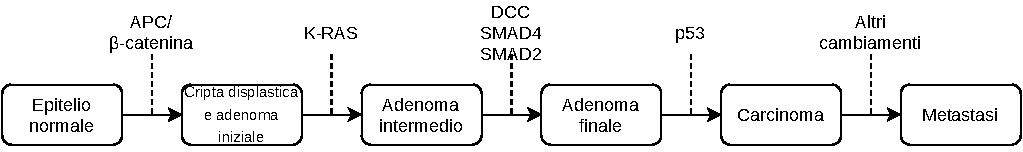
\includegraphics[scale = 0.8]{img/canc.pdf}
  \caption{Schema semplificato di una progressione del cancro al colon.}
  \label{fig:cp}
\end{figure}
Dove:
\begin{itemize}
  \item si parte con un \textit{epitelio normale} che è quello che normalmente
  abbiamo nell'intestino per tantissimi anni
  \item ad un certo punto può darsi che alcune delle cellule, normalmente alcune
  delle cellule staminali o alcuni dei progenitori semi-differenziati,
  acquisiscono una mutazione sui geni \textit{APC} e
  $\beta$\textit{-catenina}. Non sappiamo come vengono acquisite tali mutazioni 
  \item se le mutazioni rimangono fisse, ovvero le cellule che hanno la
  mutazione si riproducono senza essere rimosse dal sistema immunitario o da
  altri sistemi di controllo. Queste cellule quindi crescono in maniera
  \textbf{non ordinata}, perdendo il meccanismo di regolazione della crescita,
  avendo una \textbf{crescita displastica}. In questa situazione si ha quindi un
  \textbf{adenoma iniziale} 
  \item dopo questa situazione può darsi che una di queste cellule mutate
  acquisisca anche una mutazione sul gene \textit{K-RAS} che è un gene implicato
  nella regolazione della proliferazione delle cellule. A questo punto il
  sistema diventa un \textbf{adenoma intermedio}
  \item a questo punto le cellule possono acquisire anche le mutazioni sui geni
  \textit{DCC, SMAD4} e \textit{SMAD2} (dove si noti che \textit{DCC} sta per
  \textit{Deleted in Colorectal Carcinoma}) portando il sistema ad essere un
  \textbf{adenoma finale}
  \item se si aggiunge anche la mutazione su \textit{p53}, che è uno dei geni,
  più importante della categoria, che controlla il meccanismo di ``suicidio
  volontario'' della cellula, ovvero il processo di \textbf{apoptosi} che porta
  la cellula a smettere di riprodursi e ad essere rimossa e ``riciclata'' dal
  sistema. Se però si ha la mutazione su \textit{p53}n il sistema smettere di
  rispondere ai segnali \textit{apoptotici} e di fatto la cellula diventa
  ``immortale'' e il sistema diventa un \textbf{carcinoma}
  \item a causa di altri cambiamenti, infine, si ha la \textbf{metastasi}
\end{itemize}
Questo è stato uno dei primi modelli di progressione del tumore, in particolare
del cancro al colon. Ovviamente ora si sa che questo schema è troppo
semplificato ma è comunque un buon riferimento per il ``normale'' cancro al
colon.\\ 
Si hanno però altri tipi di cancro al colon, come il cosiddetto
\textbf{Hereditary Non-polyposis Colorectal Cancer (\textit{HNPCC})}, 
che presenta una serie diversa di mutazioni. Un'altra variante di progressione è
quella detta \textbf{Hypermethylation MSI-H}, dove la sigla sta per
\textit{MicroSatellite Instability-High}. Si hanno quindi vari tipi di
progressione anche se gli ultimi elencati hanno incidenza minore rispetto a
quello ``normale''.\\
Si hanno anche altri meccanismi relativi allo sviluppo di tumori, tra cui il
\textbf{VEGF (\textit{Vascular endothelial growth factor}) pathway} che è
relativo allo \textbf{angiogenesi}, ovvero il processo che porta alla formazione
di nuovi vasi sanguigni da altri vasi preesistenti. Un altro problema è
l'interazione delle cellule con lo \textbf{stroma}, ovvero la trama fondamentale
di un organo composto generalmente dal tessuto connettivo e dai vasi sanguigni,
e con il microambiente complessivo, dove si hanno \textit{morfogeni} presenti in
concentrazione diversa.
\section{Simulazioni 3D}
Vediamo quindi, comunque in modo molto sintetico e schematico, come fare
simulazioni tridimensionali. \\
Per modellare un \textit{tessuto tumorale} si hanno differenti \textbf{paradigmi
di modellazione} e diversi \textbf{livelli di astrazione, parametri
etc$\ldots$}.\\
Bisogna considerare, ovviamente oltre all'implementazione stessa, quali siano i
\textit{vincoli} da considerare e quali sono le grandezze da osservare. Si
vedranno:
\begin{itemize}
  \item \textbf{modelli su griglia}, detti anche \textbf{in-lattice}
  \item \textbf{modelli senza griglia}, detti anche \textbf{off-lattice} o
  \textbf{lattice-free} 
\end{itemize}
Bisogna considerare anche \textit{forze esterne, flussi, condizioni a contorno}
etc$\ldots$ \\
Sarebbe bello dare regole locali per ogni agente e osservare ex-post
l'organizzazione in colonne della riproduzione delle cellule. La cripta è una
struttura tridimensionale, a semi-cilindro, che però può essere ``srotolata'' in
un piano, ottenendo una trasformazione del problema in un problema
bidimensionale, in 2D, che è molto più semplice da studiare.
\subsection{Modelli In-Lattice}
Passiamo quindi ai \textbf{modelli su griglia}, detti appunto \textbf{modelli
  in-lattice}. Il punto chiave che differenzia i vari modelli è come modellare
gli agenti principali, nel dettaglio le varie cellule. Nei modelli
\textit{in-lattice} una cellula è modellata come una composizione di posizioni
sulla griglia e quindi non come un oggetto a se stante con una sua geometria,
come nei modelli \textbf{off-lattice}.
\subsubsection{Cellular Potts Mode}
Un modello \textit{in-lattice} molto importante è il \textbf{Cellular Potts
  Model (\textit{CPM})}, un modello che nasce nel mondo della fisica che poi è
stato riutilizzato in ambito biologico. Questo è un modello ad \textbf{automi
  cellulari}.\\
Uno dei primi usi del \textit{CPM} è quello sviluppato da Glazier e Graner, nel
1992, che è basato sul modello di Potts di meccanica statistica, ovvero uno
\textit{spin model}. Quando si misero a studiare questa simulazione lo fecero
per studiare la cosiddetta \textbf{Differential Adhesion Hypothesis
  (\textit{DAH})}, proposta da Steinberg nel 1952 e validata sperimentalmente
nel 1962 da Moscona e Moscona. Questa ipotesi è stata proposta da dei biologi ed
enuncia, in modo semplice, che se si hanno due popolazioni di cellule mischiate
(normalmente si vede con popolazioni batteriche) e queste cellule aderiscono
l'una con l'altra tra le due popolazioni allora dopo un po' il sistema tenderà a
riorganizzarsi in strati (per dire come succede quando si mischiano olio e
acqua anche se ovviamente con le cellule, che sono vive, è un discorso più
complesso).\\
L'implementazione di questo sistema viene fatta mediante il calcolo complessivo
dell'energia del sistema (indicata da Potts con $J$), energia che dipende dai
\textit{parametri di adesione} tra una cellula e un'altra, di tipo
diverso. L'energia del sistema dipende quindi dalla posizione relativa di
diverse cellule. L'evoluzione del sistema ci permette di calcolare, passo per
passo, di calcolare $J$ e di scegliere le prossime mosse per
\textbf{minimizzare} $J$. Dal punto di vista dei vincoli abbiamo quello
dell'\textbf{energia elastica} che dipende dal volume della cellula. \\
In questo sistema si osservano vari fenomeni:
\begin{itemize}
  \item \textit{auto-ordinamento delle cellule}
  \item \textit{posizionamento delle cellule}
  \item \textit{riarrangiamento e migrazione delle cellule}
\end{itemize}
Vediamo quindi la rappresentazione interna di questo sistema.\\
Abbiamo una griglia bidimensionale e l'idea chiave è quella di discretizzare lo
spazio in questa griglia. Ad ogni quadratino/pixel, identificato con le
coordinate $(i,j)$, di questa griglia si
assegnano dei numeri (come in figura \ref{fig:grid}):
\begin{itemize}
  \item $\sigma(i,j)=id$, ovvero una funzione che calcola un \textbf{id}, per
  indicare a quale cellula appartiene il pixel, 
  infatti ogni cellula è rappresentata come un insieme connesso di pixel sulla
  griglia 
  \item $\tau(\sigma(i,j))=type$, ovvero una funzione che assegna un
  \textbf{type} ad ogni cellula
\end{itemize}
\begin{figure}
  \centering
  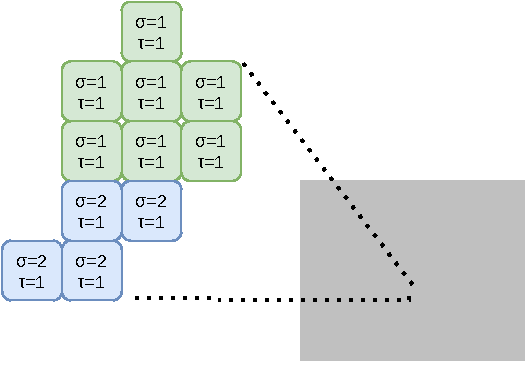
\includegraphics[scale = 1]{img/grid.pdf}
  \caption{Esempio di parte della griglia, con due cellule diverse ($\sigma=1$ e
    $\sigma=2$) dello stesso tipo ($\tau=1$)}
  \label{fig:grid}
\end{figure}
L'energia totale del \textit{CPM} è legata alla superficie delle cellule. Si ha
quindi la funzione:
\[J(\tau,\tau')\]
che rappresenta l'energia di superficie per unità di contatto tra due
cellule. L'energia è minore tra i \textit{pixel} appartenenti a due cellule
dello stesso tipo, maggiore per cellule di tipo diverso e nulla tra
\textit{pixel} della stessa cellula.
\begin{definizione}
  Definiamo l'energia totale del \textit{CPM} è definita come la somma totale
  delle energie calcolare sulle superfici delle cellule più una costante
  moltiplicata per l'energia ottenuta dall'area di una cellula, ovvero:
  \[H_{Potts}=H_{surface}+\lambda H_{Area}\]
  Dove $H_{potts}$ è un operatore Hamiltoniano e $\lambda$ è la \textbf{costante
  di rigidità} per il citoscheletro. Tale costante è usata nel ruolo di
moltiplicatore Lagrangiano. 
\end{definizione}
L'algoritmo di simulazione è molto semplice. Ad ogni passo si seleziona
randomicamente il pixel in posizione $(i,j)$ e si fa un calcolo probabilistico
per convertire l'\textit{id} $\sigma(i,j)$ nel $\sigma'$ di un pixel
confinante. Si calcola quindi la seguente probabilità (indicando con $\to$ il
passaggio di un \textit{pixel} da una cellula all'altra), per $T\neq 0$:
\[P(\sigma(i,j)\to\sigma'(i,j))=
  \begin{cases}
    e^{-\frac{\Delta H}{kT}}&\mbox{se }\Delta H>0\\
    1&\mbox{se }\Delta H\leq 0
  \end{cases}
\]
dove:
\begin{itemize}
  \item $\Delta H$ è il cambio di energia totale ad ogni step
  \item $k$ è una costante
  \item $T$ è il tempo
\end{itemize}
mentre se si ha $T=0$, avendo quindi la condizione iniziale:
\[P(\sigma(i,j)\to\sigma'(i,j))=
  \begin{cases}
    0&\mbox{se }\Delta H> 0\\
    0.5&\mbox{se }\Delta H= 0\\
    1&\mbox{se }\Delta H< 0
  \end{cases}
\]
È quindi un sistema molto semplice, ancora più semplice da implementare di
quello di Gillespie.\\
Alla fine anche questo è un algoritmo della categoria dei \textbf{metodi
  Montecarlo}, infatti passare da uno stato della griglia all'altro è fare un
passo con quel metodo.\\
Inoltre si ha anche il \textbf{gradiente DAH} che ``guida'' la probabilità che
le cellule cambino da un certo tipo ad un altro specifico tipo, facendo un
\textit{passo di Montecarlo}. Si osserva quindi il ``movimento'' atteso delle
cellule semplicemente implementando questo metodo.\\
\textbf{\textit{Su slide, parte 6, varie immagini di simulazioni, dove in base a
  diversi vingoli si ottengono separazioni nette tra tipi di cellule o miscugli,
  in assenza di particolari vincoli}.}\\
Si hanno numerosi problemi, durante le simulazioni più complesse, del
mantenimento finale della forma di determinate cellule, cosa che si risolve
tendenzialmente aggiungendo vincoli.
\subsubsection{Modello di Wong}
Vediamo quindi il \textit{modello in-lattice} per le cripte coloniche proposto
da Wong\footnote{Wong et al., Computational model of cell positioning: 
directed and collective migration in the intestinal crypt epithelium, J. Of
The Royal Soc. Interface 7, S351-363 (2010)}.\\
Questo modello ci permette di modellare la \textbf{motilità}, ovvero proprietà
dell’organismo vivente (anche unicellulare), o di una sua parte, di modificare
attivamente e in modo reversibile la propria posizione rispetto all’ambiente,
delle cellule staminali e delle cellule progenitrici all'interno delle cripte.\\
È un modello a due dimensioni dove sono stati aggiunti alcuni elementi, tra cui
il fatto che la cripta è ``srotolata'' e viene forzato esternamente tramite un
gradiente il movimento verso il \textit{lumen} da parte delle cellule.\\
Dal punto di vista dei vincoli si hanno:
\begin{itemize}
  \item si ha un \textit{termine di energia} che fa si che le cellule staminali
  rimangano fisse in posizioni predefinite
  \item regole particolari che servono a modellare la crescita cellulare, la
  divisione (asimmetrica con proliferazione e differenziazione) e
  l'\textit{apoptosi} 
  \item si ha un assunzione fondamentale di modello che ci dice che il morfogene
  più importante che viene considerato, che è quello che fa si che le cellule si
  dividano e salgano verso il \textit{lumen}, ovvero l'\textbf{adesione} sia
  data da livelli di attivazione di \textit{Eph/efrina} lungo la cripta
\end{itemize}
Il risultato finale della simulazione consente di osservare che:
\begin{itemize}
  \item l'adesione differenziale regola il posizionamento delle cellule nella
  cripta intestinale 
  \item le cellule epiteliali si muovono verticalmente verso l'alto verso il
  \textit{lumen} della cripta  
  \item il movimento è coordinato, nonostante le relativamente poche assunzioni
  \item l'omeostasi delle cellule epiteliali intestinali è mantenuta nel modello
\end{itemize}
Nonostante, si ripete, la simulazione sia semplice e con poche assunzioni.
\subsubsection{Modello Ibrido di Glazier, Graner e Hogeweg}
Un modello un poco più complesso è stato proposto da Glazier, Graner e Hogeweg e
consiste nel \textit{CPM} con l'aggiunta della modellazione della
\textbf{chemiotassi}, ovvero il fenomeno con cui i corpi cellulari, batteri ed
altri organismi unicellulari o multicellulari direzionano i loro movimenti a
seconda della presenza di alcune sostanze chimiche nel loro ambiente.\\
Questo è quindi un modello sostanzialmente \textbf{ibrido}, in quanto viene
appunto modellato il movimento esplicito delle cellule nell'ambiente.\\
Per ottenere ciò si usano dei gradienti modellati con delle \textbf{equazioni a
  derivate parziali (\textit{EDP})}. Si usano \textbf{campi discretizzati} per
descrivere la concertazione di un attrattore chimico, definiti da un insieme di
EDO all'interno di ogni cellula, che descrivono  la secrezione cellulare e
l'assorbimento della sostanza chimica, ovvero dei morfogeni. Si ha inoltre un
insieme di \textit{EDP} per calcolare la diffusione e il decadimento della
sostanza chimica, ovvero a regolare l'attivazione dei morfogeni. Si ha quindi un
\textbf{reaction-diffusion system}. Si ignora invece l'\textbf{avvezione},
ovvero il trasporto di massa o proprietà fisica che in fluidodinamica avviene
durante il moto del fluido. Si ha quindi un contributo aggiuntivo all'energia
effettiva del \textit{CPM} per tenere conto della nuova variabile di campo. \\
Il \textit{CPM} quindi è usato per modellare il movimento delle cellule, tramite
la griglia, e per tener traccia dell'energia complessiva del sistema.\\
L'uso del sistema di \textit{EDP} consente di osservare:
\begin{itemize}
  \item la chemiotassi
  \item la proliferazione delle cellule tumorali
  \item secrezione e assorbimento del \textit{fattore pro-angiogenico VEGF-A},
  che è un fattore di crescita che serve per regolare l'afflusso di nutrienti al
  tumore (???)
  \item la proliferazione di \textit{cellule neovascolari}
  \item la produzione, l'assorbimento e la diffusione di ossigeno 
\end{itemize}
Dal punto di vista software si ha un implementazione con \textbf{CompuCell3D}
(sul sito ci sono anche vari video di simulazioni etc$\ldots$).
\subsection{Modelli Lattice-Free}
Passiamo quindi ai modelli \textbf{lattice-free/off-lattice}, quindi senza
griglia. Questi modelli arrivano dal mondo della fisica.\\
Questi modelli 3D si basano sulla \textbf{partizione dello spazio di
  Voronoi-Delaunay} (anche se sarebbero nel dettaglio la \textbf{partizione di
  Voronoi} e la \textbf{triangolazione di Delaunay}). Tali modello sono modelli
\textit{biomeccanici,ibridi} e \textit{agent-based} di sistemi multicellulari.
\subsubsection{Modello di Schaller e Meyer-Hermann}
Come anticipato questo tipo di modelli deriva dal mondo della fisica, infatti il
primo modello che viene trattato è stato fatto in quell'ambiente da  Schaller e
Meyer-Hermann\footnote{Schaller, Meyer-Hermann, PHYSICAL REVIEW E 71, 051910
  s2005d}. \\
Si hanno le seguenti assunzioni in generale (comuni anche ad altri modelli): 
\begin{itemize}
  \item la \textbf{cellula} è un \textit{corpo semi-sferico} e la forma varia da
  sferica in soluzione sottile a \textit{convessa poliedrica di Voronoi} in
  tessuti densi. Questa modellazione rende tutto più semplice
  \item dal punto di vista delle \textbf{forze} si hanno:
  \begin{itemize}
    \item la \textit{forza elastica} tra cellule
    \item \textit{interazioni/forze di adesione e frizione} tra cellule
    \item \textit{interazioni/forze di adesione e frizione} tra cellula e
    substrato 
  \end{itemize}
  \item lo \textbf{stato della cellula} è rappresentato da:
  \begin{itemize}
    \item posizione
    \item concentrazione nella membrana cellulare di recettori e ligandi. Questa
    informazione è necessaria per parlare di adesione
    \item il ciclo interno alla cellula
    \item altre caratteristiche, rappresentate da costanti, utili per le
    interazioni elastiche e di adesione. Tali costanti sono dipendenti dal tipo
    preciso di cellula 
  \end{itemize}
  \item per la \textbf{dinamica} con cui le cellule si muovono nello spazio si
  usano \textbf{equazioni di Newton} per le singole cellule, corredate da
  \textit{EDP} per modellare campi in cui si muovono le cellule, dove ci sono
  processi di reazione e diffusione che coinvolgono nutrienti, come Ossigeno e
  Glucosio. Le \textit{EDP} determinano quindi la distribuzione spazio-temporale
  dei nutrienti 
  \item si hanno infine \textbf{segnali di crescita} che fanno si che aumenti la
  \textit{biomassa} (aumentando di volume fino ad un certo limite fino alla
  divisione), quando le cellule consumano i nutrienti
\end{itemize}
La \textbf{triangolazione di Delaunay} viene utilizzata per fornire in modo
efficiente l'elenco dei prossimi vicini per l'interazione cellula-cellula.\\
La \textbf{partizione di Voronoi} e la \textbf{triangolazione di Delaunay} sono
duali e sono usate per rappresentare in modo approssimato cellule e tumori
sferici. Si hanno estensioni per un numero $n$ di dimensioni.\\
Parliamo dell'estensione bidimensionale. Si hanno dei punto in un piano che
vengono connessi tra loro con linee tratteggiate, come in figura
\ref{fig:tri}. Non si possono avere linee che si intersecano tra loro e tali
linee rappresentano appunto la \textit{triangolazione di Delaunay}. Ci sono
algoritmi che costruiscono la triangolazione in modo efficiente, basandosi su
una \textit{scan-line} e man mano che si ha la scansione si costruisce la
triangolazione. Si procede poi prendendo il punto medio di ogni segmento e
costruisco un poligono in grassetto che passa coi suoi lati attraverso tali
punti medi. La zona delimitata da questo poligono è la \textbf{cellula di
  Voronoi} e corrisponde alla costruzione  \textit{della partizione di Voronoi}
nel piano. Ovviamente la partizione dipende dalla posizione dei punti e si
possono generare più partizioni, dove ogni partizione contiene un punto di
quelli di partenza e tutti i punti ipotetici della ragione hanno quel tal punto
come punto più vicino. Si possono ottenere così approssimazioni accettabili.\\
\begin{figure}
  \centering
  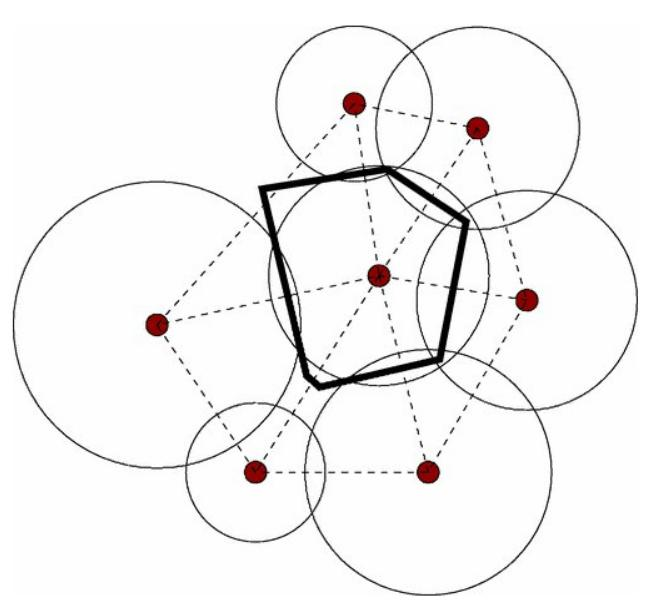
\includegraphics[scale = 0.3]{img/tri.jpg}
  \caption{Esempio di triangolazione bidimensionale dove viene specificata la
    partizione del punto rosso centrale, tutti i punti che posso prendere in
    quell'area sono più vicini al punto rosso centrale che a qualsiasi altro
    punto rosso della figura.}
  \label{fig:tri}
\end{figure}
Rappresentare le cellule con questi \textbf{diagrammi di Voronoi} facilita di
molto la computazione di misure e quantità di interesse per capire come si
evolve il sistema, potendo identificare schematicamente le forze, atte a
calcolare poi i cambiamenti nella posizione delle cellule (con le forze che
producono una forza risultante che muove la cellula in certe direzioni), ma
anche a poter rappresentare la suddivisone delle cellule. Le varie forze vengono
calcolate come agenti sulle facce della superficie calcolata (si associa un
singolo valore ad ogni superficie, nel punto medio di ogni lato) e quindi si può
computare meglio come ottenere la risultante. È anche questa un'approssimazione
accettabile (anche perché tali calcoli su una curva non sarebbero
gestibili). Tali calcoli, come quello della forza risultante dipende poi dal
calcolo di integrali non banali. Per la divisione si ha che si costruisce un
nuovo \textit{diagramma di Voronoi}, avendo che da un punto se ne producono
due. Si hanno questioni algoritmiche non banali in quanto, dato un insieme di
punti, su un piano o anche in uno spazio 3D, è semplice costruire il
\textit{diagramma di Voronoi/triangolazione di Delaunay}, avendo algoritmi noti,
mentre si hanno problemi quando si ha uno spazio partizionato e si vuole
modificare la struttura del sistema. Tutti gli algoritmi noti infatti agiscono a
livello \textit{globale} ma per modellare una divisione cellulare ho una
modifica \textit{locale} al \textit{diagramma di Voronoi}, non cambiando quasi
nulla nelle aree lontane. È quindi inefficiente ricalcolare tutto ad ogni
divisione cellulare e quindi si hanno varie soluzioni algoritmiche non
banali, di natura numerica, che permettono di fare aggiornamenti locali in modo
abbastanza efficiente. La letteratura dedicata si ritrova sotto il nome di
\textbf{dynamic update Voronoi diagrams} e spesso trattano soprattutto
dell'errore introdotto dagli algoritmi, usando calcoli numerici non semplici da
gestire, avendo problematiche dal punto di vista della \textbf{robustezza degli
  algoritmi}. \\
Tali simulazioni hanno anche avuto uso in \textit{meccanica
muscolare} e \textit{meccanica scheletrica}, oltre che a vari problemi
ingegneristici (turbine, centrali nucleari etc$\ldots$).\\
Questo modello include la \textbf{proliferazione}, secondo regole predefinite, e
si voleva modellare la dinamica della popolazione e il mantenimento della
morfologia sferoide del tumore, studiando i meccanismi per l'induzione della
\textbf{necrosi cellulare}.
\subsubsection{Modello di Buske e Galle}
Un modello diverso è quello proposto da Buske, Galle et al\footnote{P. Buske,
  J. Galle, et al, A Comprehensive Model of the 
Spatio-Temporal Stem Cell and Tissue Organisation in the Intestinal
Crypt, PLoS Comput Biol, vol. 7, no. 1, 2011}, tra cui Drasdo. \\
Questo è un modello biomeccanico \textit{agent-based} per sistemi
multicellulari. Le cellule sono trattate come corpi elastici deformabili, pur
tenendo a mantenere di base forma sferica, in grado di:
\begin{itemize}
  \item muoversi
  \item dividersi
  \item differenziarsi
  \item ``comunicare'' tra loro
\end{itemize}
La dinamica viene rappresentata tramite le \textbf{equazioni di Langevin}.\\
Si usano variabili di stato dinamiche per:
\begin{itemize}
  \item la posizione delle cellule
  \item la dimensione delle cellule
  \item il vettore dello stato interno (\textit{internal state vector}) per
  l'\textit{internal activity status}, con ad esempio la trascrizione dei geni
  target, con, ad esempio, il \textit{Wnt-pathway} o il \textit{Notch-pathway}
\end{itemize}
La forma delle cripte intestinali è quella di una ``scafallatura'' 3D abbastanza
fedele alla vera forma di una cripta.\\
Il vettore dello stato interno può essere cambiato tramite la dinamica esterne
alle cellule, avendo dinamica delle posizioni e delle dimensioni. Non si hanno
invece equazioni di dinamica per lo stato interno, non avendo, ad esempio,
relazioni metaboliche e questo è importante visto che spesso si vuole accoppiare
la dinamica interna di una cellula con quella esterna, modellando sia i processi
intra-cellulari che inter-cellulari. La scala dei tempi in cui questi processi
avvengono è però abbastanza diversa avendo che la simulazione potrebbe
rallentare molto.\\
Dal punto di vista delle forze si hanno quindi le interazioni tra cellule e le
interazioni di una cellula con il substrato, in termini di adesione e
frizione. \\
Il modello puntava quindi a descrivere lo stato stazionario delle cripte
coloniche, stato in cui si ha una \textit{dinamica stazionaria}, dove si ha la
divisione e la differenziazione delle cellule. Si parla di \textbf{omeostasi},
la capacità di autoregolazione degli esseri viventi, importantissima per
mantenere costante l'ambiente interno nonostante le variazioni dell'ambiente
esterno, ovvero l'\textit{equilibrio dinamico}.\\
Il modello tiene traccia della crescita delle cellule, della divisione e della
differenziazione delle stesse, per tutte e tre le cose con regole predefinite
scelte tramite studi sperimentali. A questi vincoli si aggiungono:
\begin{itemize}
  \item dal punto di vista dell'energia di interazione abbiamo:
  \begin{itemize}
    \item interazione di adesione
    \item l'energia di deformazione per contatto, secondo il modello di Hertz
    \item energia di compressione elastica per le sfere 
  \end{itemize}
  \item per le forze si ha che essere sono sia deterministiche che stocastiche,
  anche se i termini stocastici sono solamente \textit{termini di rumore}
  \item si assume l'ancoraggio al substrato. Le cellule interagiscono con la
  \textit{membrana basale}, ovvero la struttura laminare specializzata della
  matrice extracellulare di spessore compreso tra 70 e 300 \textit{nm} che fa da
  interfaccia tra un tessuto connettivale e un tessuto non connettivale, 
  tipicamente epiteli. Questa interazione però avviene se la loro distanza è
  minore di quella del loro raggio e si ha che esse sono rimosse dal sistema
  della cripta se si perde il contatto con la membrana basale
\end{itemize}
Si ha inoltre un \textit{ciclo cellulare} programmato, per controllare:
\begin{itemize}
  \item la regolazione e il controllo della crescita cellulare
  \item la forma di inibizione della crescita mediata dal contatto tra cellule
  (???) 
  \item l'arresto del ciclo cellulare in dipendenza dal contatto tra una cellula
  e il substrato
  \item la morte cellulare programmata in dipendenza dal contatto tra una
  cellula e il substrato, simulando quindi processi apoptotici
\end{itemize}
Questo modello consente di osservare:
\begin{itemize}
  \item omeostasi del sistema
  \item l'auto-organizzazione spazio-temporale del tessuto
  \item la migrazione delle cellule verso il \textit{lumen} della cripta
  \item la riorganizzazione delle cellule nel sistema
\end{itemize}
Tutto questo studiando \textit{sensitività, stabilità} e \textit{flessibilità}
al cambiamento dei livelli di attivazione dei segnali di \textit{Wnt} e
\textit{Notch}. La proliferazione e la differenziazione dipendono infatti
dall'attivazione del \textit{Wnt-pathway} e del \textit{Notch-pathway}, dalla
posizione delle cellule, tramite il \textit{Wnt-gradient} e il
\textit{Notch-gradient} e dalla curvatura della membrana basale del substrato.
\subsubsection{Modello di Drasdo}
Un altro modello è quello detto \textbf{modello di Drasdo}\footnote{J. Galle,
  G. Aust, G. Schaller, T. Beyer, and D. 
Drasdo, “Individual cell-based models of the spatial-
temporal organization of multicellular systems--
Achievements and limitations,” Cytometry, vol. 69,
no. 7, pp. 704–710, 2006.}.\\
L'articolo indicato contiene questo modello anche se in realtà Drasdo aveva in
primis introdotto un modello 1D, usando ``stringhe di cellule'', per le
\textit{cripte intestinali} e aveva ha 
introdotto le prime idee sui modelli \textit{agent-based} individuali, ovvero
aveva introdotto i modelli \textit{off-lattice/lattice-free}. Solo dopo Galle
ha iniziato ad applicare tali idee.
\subsection{Obiettivi Futuri}
Dopo aver visto alcuni modelli è interessante pensare a qualche obiettivo
futuro, elencando le varie \textit{problematiche aperte}. Alla base si ha sempre
la ricerca di interazioni tra i diversi livelli di simulazione e tra le idee
possibili abbiamo:
\begin{itemize}
  \item combinare il modello di Galle per le cripte con l'idea di Schaller e
  Meyer-Hermann per la rappresentazione delle cellule tramite \textit{partizioni
    di Voronoi} e \textit{triangolazione di Delaunay}
  \item combinare il modello di Wong delle cripte dinamiche con il modello di
  Hogeweg per la diffusione dei nutrienti e le reazioni, nel caso 2D. Si
  otterrebbe un modello bidimensionale che sarebbe quello di Wong con
  l'aggiunta di \textit{EDP} 
  \item combinare il modello di Wong delle cripte dinamiche con il modello di
  Hogeweg per la diffusione dei nutrienti e le reazioni, nel caso 3D. Si
  otterrebbe un modello tridimensionale che sarebbe quello di Wong con
  l'aggiunta di \textit{EDP} ma bisognerebbe capire come implementare
  \textit{CPM} in una forma per le cripte non cilindrica, come nel caso del
  modello di Galle delle cripte. Qui la situazione diventa davvero complessa
\end{itemize}
Gli sforzi futuri dovrebbero puntare alla formazione di modelli ragionevoli in
cui stimoli meccanici e processi intracellulari biochimici sono accoppiati in un
quadro dinamico unificato, con un modello che permetta di ragionare in modo
accettabile su tutti questi aspetti nel loro complesso. I modelli di crescita,
divisione e differenziazione cellulare dovrebbero essere in grado di descrivere,
a livello microscopico, l'esatto stimolo meccanico che innesca la crescita e
successivamente le reazioni biochimiche che portano alla divisione e alla
differenziazione. Inoltre questi modelli dovrebbero chiarire come le cellule
percepiscono i segnali meccanici e li convertono in quelli chimici che alla fine
inducono una risposta biologica come la crescita. Bisognerebbe quindi modellare
il meccanismo sensoriale delle cellule, che dal punto di vista biologico avviene
tramite le membrane e permette di far capire ad una cellula cosa accade attorno,
ovvero cosa c'è sulle membrane delle cellule vicine, vario segnali molecolari
presenti nell'ambiente in cui le cellule si trovano etc$\ldots$\\
Al momento, la ristretta conoscenza complessiva delle diverse reazioni
biochimiche coinvolte nella crescita, divisione e differenziazione cellulare
rende molto difficile fornire un modello meccanico macroscopico che spieghi
tutti i diversi passaggi microscopici coinvolti nei pathway di trasduzione del
segnale. Non conosciamo tutti i dettagli dell'interazione tra cellule. Quindi la
ricerca di settore si concentra attualmente nella 
\textbf{modellazione multiscala (\textit{multiscale modelling})}, cercando di
risolvere quindi il problema della differenza di scale temporali, per la
rappresentazione congiunta di dinamiche intra-cellulari e inter-cellulari. Il
problema del \textit{multiscale modelling} non è molto diverso dal problema
visto parlando del \textit{tau-leaping} per Gillespie, facendo un passo ad una
certa scala cercando di assicurarsi che ci siano delle condizioni che
garantiscano che il passo non fa ``sforare troppo'' da quanto avrei ottenuto
muovendomi con i micro-passi a scale inferiori. In questo caso ovviamente gli
strumenti matematici per ottenere questo risultato sono assai più variegati e
complessi.
\chapter{Flux Balance Analysis}
Finora sono state viste diverse tecniche di simulazione. Si presenta ora una
tecnica di analisi, detta \textbf{Flux Balance Analysis (\textit{FBA})}.\\
In questo contesto si analizzano i sistemi biologici da un punto di vista
diverso, ovvero quello del \textbf{metabolismo}. Si ricorda che il metabolismo
di un sistema è rappresentato da un insieme di \textit{reazioni
  metaboliche}, cioè cioè dalla\textit{ matrice stechiometrica} dell'insieme
delle reazioni. Nel dettaglio con la \textit{FBA} si studiando i \textbf{flussi}
di sostanze chimiche nel sistema\footnote{K. Raman and N. Chandra, “Flux balance
  analysis of biological systems: applications and challenges,” Briefings in
Bioinformatics, vol. 10, no. 4, pp. 435–449, Jun. 2009.}\footnote{J. D. Orth,
I. Thiele, and B. Ø. Palsson, “What is flux balance analysis?,” Nature
Publishing Group, vol. 28, no. 3, pp. 245–248, Mar. 2010.}.
\section{Pathway Metabolici}
Il punto chiave è
che rappresentare il metabolismo, con tutti i suoi pathway (eventualmente poi
rappresentati tramite insiemi di equazioni), è veramente
complesso per questo lo studio viene fatto \textit{in silico}, nell'ambito della
\textbf{biologia computazionale}.\\
Il \textbf{metabolismo cellulare} a partire dal cibo e tramite \textit{pathway
  catabolici} produce:
\begin{itemize}
  \item energia
  \item componenti utili alla sintesi delle cellule
  \item calore
\end{itemize}
e, tramite i primi due e i \textit{pathway anabolici}, vengono prodotte varie
macromolecole.
\begin{definizione}
  Si definisce \textbf{pathway metabolico} una sequenza, o meglio un
  \emph{grafo}, di \emph{reazioni metaboliche}.
\end{definizione}
Un esempio di pathway metabolico è quello già introdotto della
\textbf{glicolisi} che, a partire da una molecola di Glucosio produce
\textit{ATP} e due molecole di piruvato, che, nel caso di un processo di
respirazione/fermentazione anaerobica, diventa lattato.\\ 
Un altro pathway importante, che lavora in combinazione con la
\textit{glicolisi}, è \textbf{ciclo di Krebs}, detto anche \textbf{ciclo TCA
  (da \textit{tricarboxylic acid cycle})}, un meccanismo metabolico presente
in praticamente tutti gli organismi, atto a gestire l'ossigeno fornito dalla
respirazione. \\
Se vengono presi tutti i pathway metabolici e vengono rappresentati insieme si
ottiene la \textbf{rete metabolica}, detta anche \textbf{metaboloma}, di cui una
sezione è visibile in figura \ref{fig:met}.\\
\begin{figure}
  \centering
  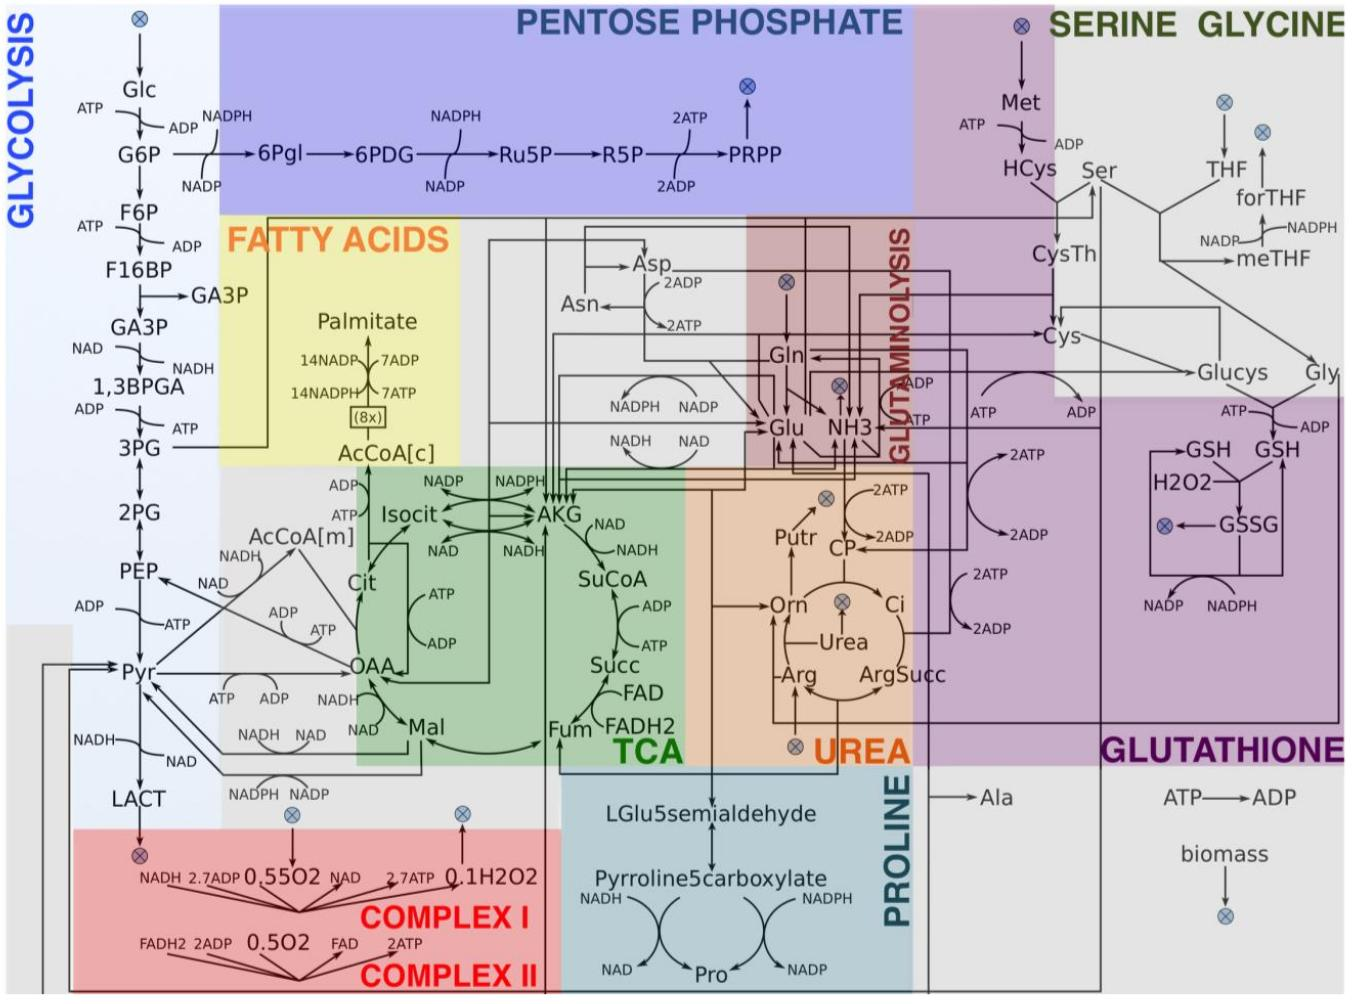
\includegraphics[scale = 0.25]{img/met.jpg}
  \caption{Sezione del metaboloma, rappresentata in modo ``astratto'', con una
    dozzina di pathway connessi, tra cui i già citati pathway della glicolisi e
    del ciclo di Krebs.} 
  \label{fig:met}
\end{figure}
Un altro aspetto che bisogna considerare quando si vuole rappresentare sistemi
biologici di questo tipo è il livello di astrazione. Una stessa reazione o uno
stesso evento biologico può infatti essere rappresentato in modo più granulare o
più astratto, anche se sottostante si ha comunque lo stesso comportamento.
\newpage
Ad esempio potremmo avere la seguente rappresentazione più granulare:
\begin{figure}[H]
  \centering
  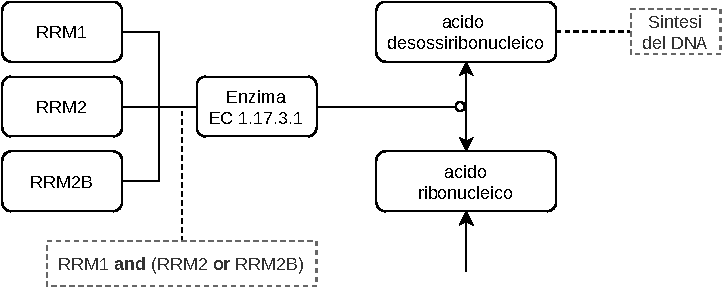
\includegraphics[scale = 0.8]{img/ab.pdf}
\end{figure}
Dove si ha una regola booleana per l'enzima/gene che coinvolge l'enzima
\textbf{RRM1 (\textit{Ribonucleotide Reductase Large Subunit})}, che è una
sub-unità catalitica, l'enzima \textbf{RRM2 (\textit{Ribonucleoside-diphosphate
    reductase subunit})} e l'enzima \textbf{RRM2B (\textit{p53-Inducible
    Ribonucleotide Reductase subunit})}, dove le ultime due sono sub-unità
regolatorie isoformi. Si nota che l'uso di \textit{funzioni booleane} rende
semplice il passaggio dalla modellazione astratta al software.\\
Tutto questo, che non approfondiamo dal punto di vista biologico, però può
essere rappresentato in modo più astratto nel seguente modo, ad esempio:
\begin{figure}[H]
  \centering
  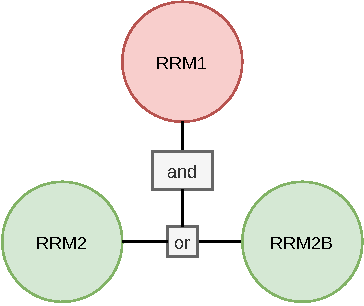
\includegraphics[scale = 0.8]{img/ab2.pdf}
\end{figure}
dove si ha astrazione a \textit{livello molecolare}, a cui si
potrebbe aggiungere la conformazione delle proteine.\\
Si hanno vari motivi per studiare il metabolismo, andando oltre il mero studio
di sequenze tipico della \textbf{bioinformatica}, infatti la deregolamentazione
del metabolismo cellulare è coinvolta in molte malattie, come:
\begin{itemize}
  \item cancro, dove si noti le cellule usano anche pathway differenti da
  quelli standard per la produzione di energia. In merito si ha anche lo studio
  dei tumori sia dal punto di vista interno alla cellula, \textit{intra-tumor},
  che in un insieme di cellule, \textit{inter-tumor}
  \item diabete
  \item obesità
  \item malattie legate al fegato grasso
  \item Parkinson
  \item Alzheimer
\end{itemize}
Ma lo studio è anche legato ad analizzare gli effetti dell'invecchiamento,
infatti il metabolismo cambia con l'avanzare degli anni.\\
Un altro motivo per cui si studia il metabolismo è l'ingegnerizzazione dello
stesso, specialmente parlando di batteri. Si è visto con l'esempio del
Repressilator come si possa indurre una popolazione a compiere una certa azione.
Studi simili sui batteri hanno portato al loro uso per la produzione di: 
\begin{itemize}
  \item prodotti chimici di base
  \item sostanze di \textit{chimica fine}
  \item farmaci
  \item combustibili
\end{itemize}
Per capire, all'interno del nostro sistema, quali siano le parti più attive
possiamo quindi studiare il \textit{flusso}.
All'atto pratico:
\begin{itemize}
  \item \textbf{si può} misurare il \textbf{metaboloma}, misurando la
  concentrazione dei \textit{metaboliti}, ovvero un qualsiasi prodotto terminale
  o intermedio del metabolismo, ad un certo tempo $t$
  \item \textbf{non si può} misurare il \textbf{flussoma}, ovvero i flussi
  metabolici nell'intervallo $\Delta t$ 
\end{itemize}
\begin{definizione}
  In questo contesto definiamo \textbf{flusso} come il tasso delle reazioni ``in
  avanti'' meno il tasso delle reazioni ``all'indietro'':
  \[flux=rate_{forward}-rate_{backward}\]
\end{definizione}
Sarebbe comunque molto interessante per studiare \textit{metaboloma} e
\textit{fluxome}, per capire quali reazioni sono \textbf{up-regolate} e quali
\textbf{down-regolate}.
\section{Programmazione Lineare}
Si hanno quindi varie soluzioni modellistiche, che si contrappongono alle
difficoltà di una vera e propria simulazione (tra cui capire le costanti,
scegliere i parametri, eseguire la vera e propria simulazione etc$\ldots$):
\begin{itemize}
  \item \textbf{modellazione statica}
  \item \textbf{modellazione dinamica}
  \item \textbf{modellazione dello steady-state}, che è una via di mezzo che
  assume lo stato di equilibrio del sistema, permettendo un'analisi più semplice
\end{itemize}
In questo contesto viene anche utilizzata una delle nozioni base della
\textit{Ricerca Operativa}, ovvero la ricerca di ottimo tramite approssimazione
con \textbf{programmazione lineare}. Si hanno quindi:
\begin{itemize}
  \item la matrice stochiometrica $S$, dove le colonne sono le reazioni (magari
  nel caso semplice $reazione\to prodotto$) e le colonne sono i metaboliti
  \item lo steady state $S\cdot v = 0$
  \item i vincoli di flusso:
  \[v_{min}<v<v_{max}\]
  che rappresentano diversi tipi di flusso:
  \begin{itemize}
    \item \textit{flussi in entrata}, tramite vincoli sui nutrienti
    \item \textit{flussi interni}, tramite vincoli termodinamici e vincoli sul
    tasso sul \textit{reaction rate}
    \item \textit{flussi di secrezione}, per rappresentare che il metabolismo è
    in grado di accumulare, rappresentando quindi la crescita e i suoi vincoli
  \end{itemize}
\end{itemize}
Una volta fatti i vari conti conti con al programmazione lineare otteniamo
un'area dei \textbf{possibili fenotipi}, ovvero l'area delimitata dai vincoli
stessi.
\newpage
Prendiamo ora un piccolo esempio:
\begin{figure}[H]
  \centering
  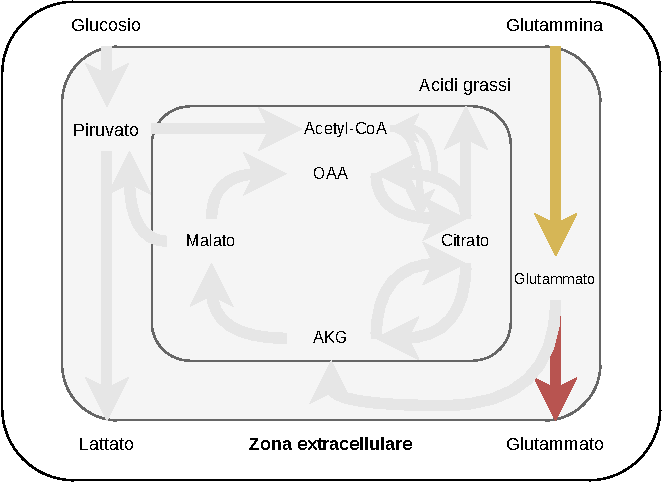
\includegraphics[scale = 0.8]{img/toy.pdf}
\end{figure}
dove eventuali frecce gialle rappresentano il flusso, quindi la
quantità di sostanza trasformata per unità di tempo, mentre se rosse
rappresentano il massimo flusso possibile (questa notazione può variare, ad
esempio usando frecce non piene per il primo caso).\\
Ovviamente, a seconda di dove si hanno i flussi, si possono rappresentare vari
comportamenti e, nel dettaglio di questo esempio, si potrebbe anche creare un
ciclo:
\begin{figure}[H]
  \centering
  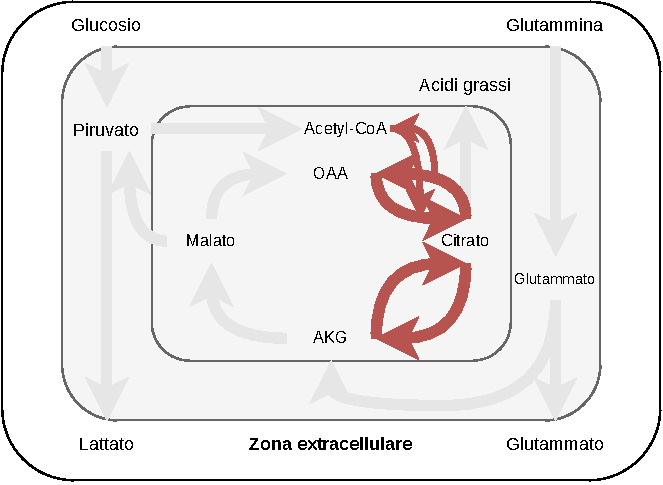
\includegraphics[scale = 0.7]{img/toy2.pdf}
\end{figure}
Ottenendo un Ciclo di flusso termodinamicamente irrealizzabile.
Una tale situazione deve essere quindi risolta modificando o aggiungendo vincoli
al sistema.\\
A tale sistema si aggiungono degli scambi necessari. Le reazioni di scambio sono
definite tramite due quantità e questo, per la reazione $R$, si indica con
$R\iff$: 
\begin{enumerate}
  \item \textbf{uptake (\textit{assorbimento})}: la rimozione dall'ambiente
  extracellulare, ovvero il \textit{flusso negativo}. Il valore è compreso tra
  $-\infty$ e $0$ 
  \item \textbf{secretion (\textit{secrezione})}: l'inserimento nell'ambiente
  extracellulare, ovvero il \textit{flusso positivo}. Il valore è compreso tra
  $0$ e $+\infty$ 
\end{enumerate}
Si ottiene quindi:
\begin{figure}[H]
  \centering
  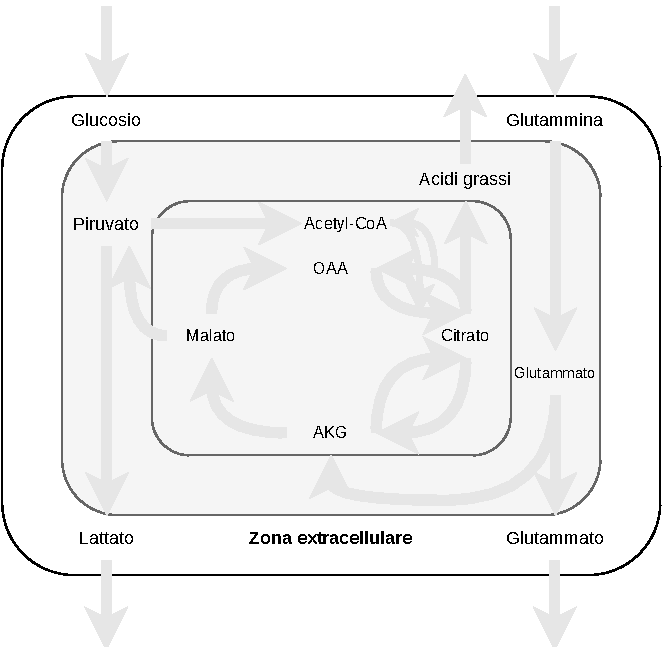
\includegraphics[scale = 0.58]{img/toy3.pdf}
\end{figure}
A questo punto possiamo avere molteplici steady state rappresentabili in questo
modo. Ad esempio potremmo rappresentare uno (ma non l'unico) steady state per
l'assorbimento forzato di Glucosio:
\begin{figure}[H]
  \centering
  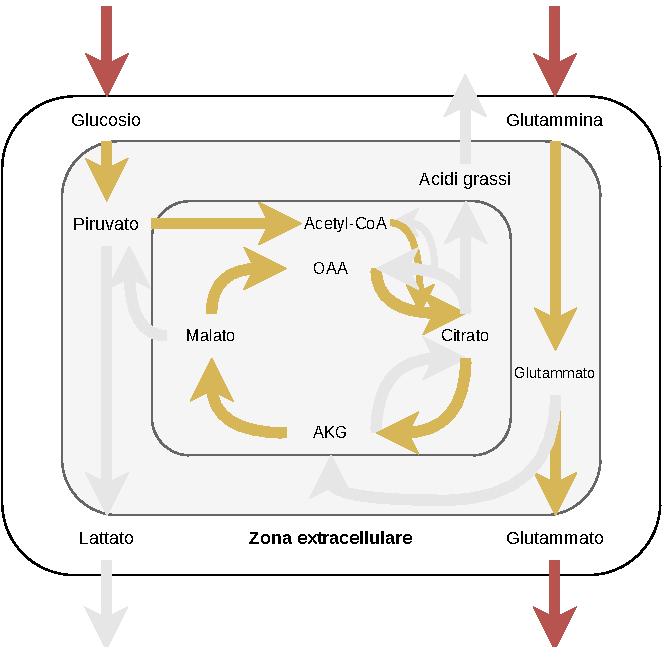
\includegraphics[scale = 0.5]{img/toy4.pdf}
\end{figure}
\textbf{\textit{Su slide lezione 7 altri possibili steady state}}.
\newpage
Vediamo quindi come funziona una m\textbf{odellazione basata su vincoli} e la
\textbf{Flux Balance Analysis (\textit{FBA})}. Si ha:
\begin{itemize}
  \item si parte con la ricostruzione metabolica su scala genomica, studiando le
  reazioni e capendo come funzionino i vari pathway
  \item si continua rappresentando matematicamente le reazioni metaboliche e i
  vincoli. Nel dettaglio si usa una matrice stochiometrica $S$, a cui vengono
  aggiunte delle colonne in fondo a destra per le ``variabili'' di interesse,
  per esempio biomassa, Glucosio, Ossigeno etc$\ldots$. Si moltiplica tale
  matrice per il vettore $v=\{v_1,\ldots, v_n,v_1',\ldots,v_m'\}$ contenente i
  vari flussi più i flussi legati alle variabili di interesse (indicate con i
  vari $v'$). Si calcola quindi $S\cdot v=0$, si ha quindi un
  sistema lineare omogeneo in quanto si studia lo steady state
  \item il bilancio di massa definisce un sistema di equazioni lineari a partire
  da $S\cdot v=0$, che sono i vincoli del sistema da studiare con la
  programmazione lineare
  \item si definisce una funzione obiettivo su cui cercare l'ottimo del tipo:
  \[z=c_1\cdot v_1+c_2\cdot v_2\cdots\]
  e si usa $z$ per predire i valori di intesse, ad esempio per la biomassa, si
  userebbe banalmente $z=v_{biomassa}$, con $v_{biomassa}$ che è uno dei $v_i'$
  indicati sopra
  \item si calcola infine il flusso che massimizza $z$ tramite programmazione
  lineare
\end{itemize}
La forma generica, nel caso di ricerca di un massimo, di questa funzione
obiettivo e dei suoi vincoli è: 
\begin{equation*}
  \begin{array}{rrclcl}
    \displaystyle \max & \multicolumn{3}{l}{z=c^Tv} \\
    \textrm{s.t.} & S\cdot v & = & 0 \\
                       & \alpha & \leq & v_i & \leq& \beta \\
  \end{array}
\end{equation*}
Si ha che la funzione obiettivo può anche essere riscritta come:
\[z=\sum_i c_i\cdot v_i=c\cdot v\]
dove si identificano meglio:
\begin{itemize}
  \item i pesi $c_i$
  \item i coefficienti obiettivo $v_i$
\end{itemize}
Ovviamente ci sono situazioni in cui l'ottimo è un massimo e altre in cui
l'ottimo è un minimo, infatti, tra le altre, potremmo voler studiare funzioni
che:
\begin{itemize}
  \item minimizzano il consumo di Glucosio
  \item massimizzano la produzione di composti chimici e biocarburanti
  \item massimizzare la crescita
  \item massimizzare la biomassa
  \item massimizzare/minimizzare qualche particolare aspetto legato alle reazioni
\end{itemize}
Per esempio se volessi massimizzare l'acido grasso otterrei, sempre nell'esempio
``giocattolo'' di prima, un sistema di questo tipo:
\begin{figure}[H]
  \centering
  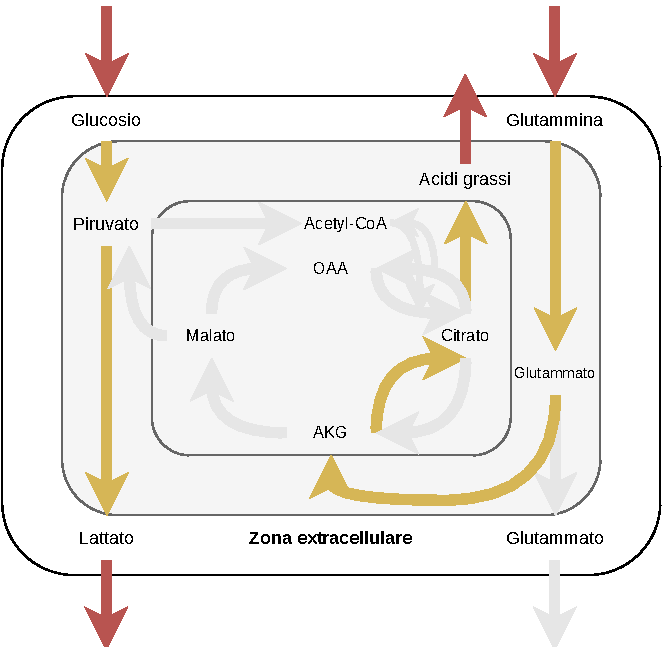
\includegraphics[scale = 0.7]{img/toy5.pdf}
\end{figure}
Questi studi vengono usati ad esempio per esperimenti con il
\textnormal{chemostato}, ovvero un reattore biologico (o bioreattore) ideale che
lavora in condizioni di stato stazionario.\\
\textit{Nel reattore biologico, i microrganismi presenti usano il substrato
  presente nella portata di alimentazione per la crescita. Le condizioni
  stazionarie implicano da un lato che il substrato non si accumuli all'interno
  del reattore e, dall'altro, che la biomassa prodotta sia uguale a quella
  allontanata per unità di tempo.}\\
In questo contesto si fanno esperimenti sui vincoli, come la produzione e il
consumo di nutrienti, studiando ad esempio come massimizzare la crescita,
cercando di predire questi fenomeni in \textit{dry-lab}.\\
Si ha quindi che la \textit{programmazione lineare} è usata insieme alla
\textit{FBA} per assicurare la fattibilità dei flussi, per ottimizzare la
funzione che è combinazione lineare dei prodotti del sistema e per ottimizzare
le condizioni a contorno. Ovviamente tale studio può risultare complesso dal
punto di vista computazionale. Solitamente si parte con il famoso
\textbf{algoritmo del simplesso}, che solitamente è sufficiente anche se può
diventare di complessità esponenziale in certi casi. In caso di ``fallimento''
di questa soluzione, al variare anche della presenza di variabili discrete o
continue, si procede selezionando altri algoritmi (ed eventualmente altri
risolutori software).
\section{Questioni Avanzate per FBA}
Come abbiamo visto usando i metodi di programmazione lineare si ottiene una
soluzione ottima ma questo aspetto può essere a volte limitante. Il problema da
affrontare è essenzialmente quello di classificare/scegliere i diversi ``stati''
metabolici che emergono in un'analisi, al cambiare, ad esempio, dei parametri o
della funzione obiettivo. Questo tipo di discorso diventa interessante parlando
di \textbf{metabolic rewiring (\textit{ricablaggio metabolico})} nell'ambito del
cancro. \\
La \textit{FBA} può essere usata in molti modi, con varie applicazioni ed
estensioni, come riassunto in figura \ref{fig:fba}\footnote{K. Raman and
  N. Chandra, “Flux balance analysis of 
  biological systems: applications and challenges,” Briefings in
  Bioinformatics, vol. 10, no. 4, pp. 435–449, Jun. 2009.}. Tali problemi
variano al cambiamento dei pesi e della funzione obiettivo, alcuni di essi sono
risolubili in parte numericamente etc$\ldots$ e tutti questi sono aspetti che
devono essere studiati e approfonditi di volta in volta.\\
\begin{figure}
  \centering
  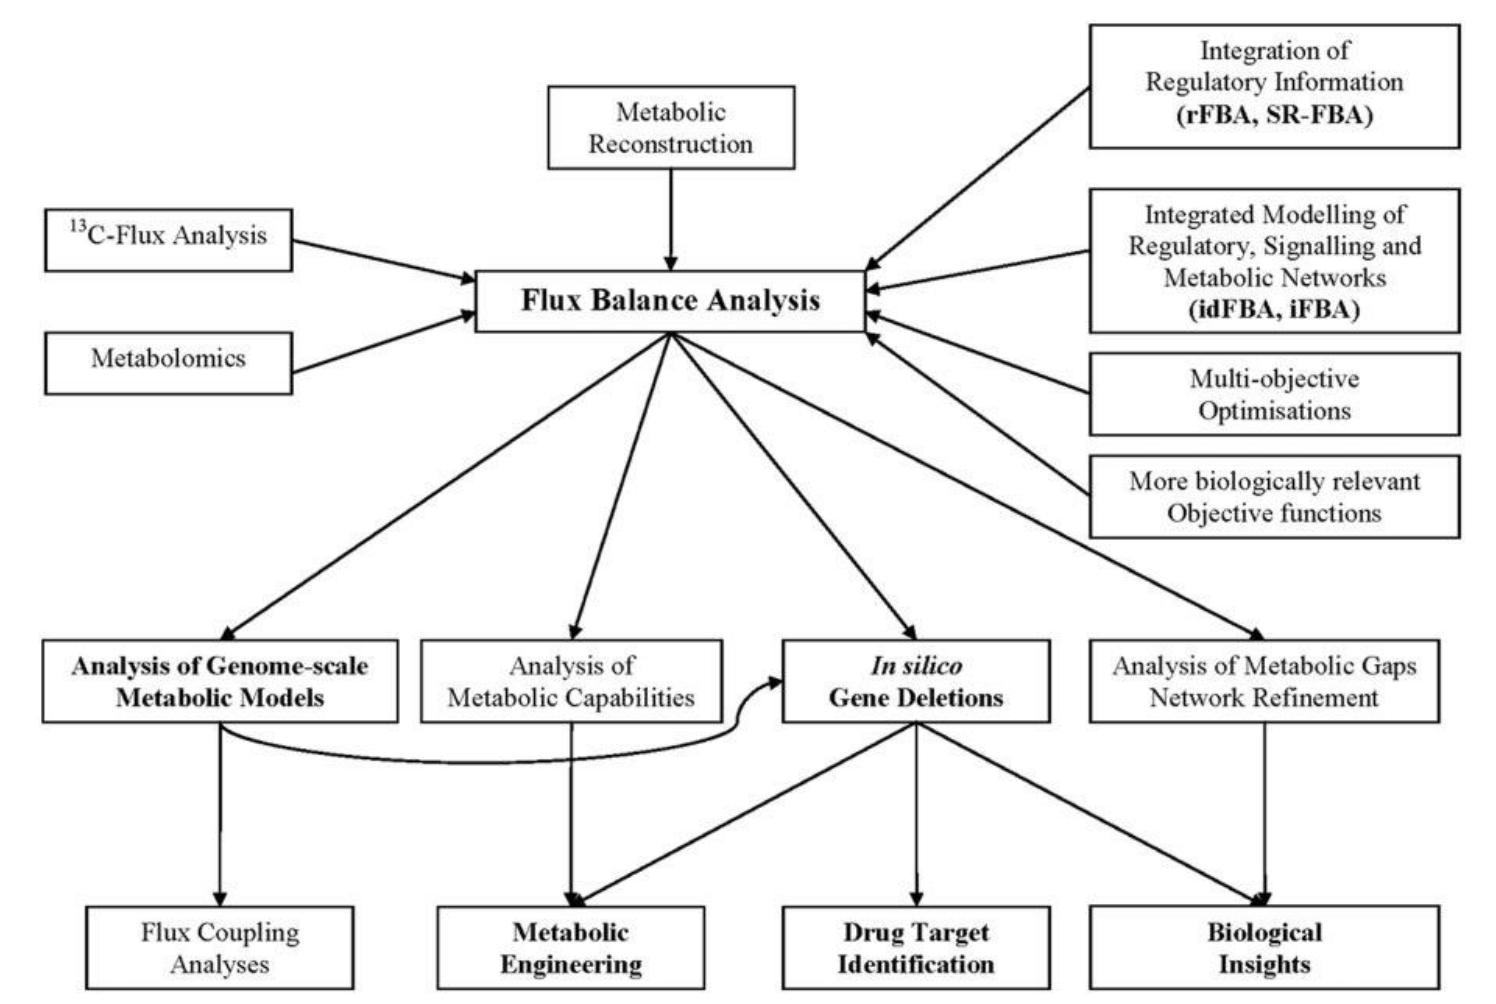
\includegraphics[scale = 0.2]{img/fba.jpg}
  \caption{Vecchio schema riassuntivo degli usi della \textit{FBA}.}
  \label{fig:fba}
\end{figure}
Dal punto di vista della programmazione lineare si hanno varie categorie di
risolutori per il caso continuo ma possiamo tutte racchiuderle in due
macro-categorie, considerando comunque che dal punto di vista della biologia
computazionale sono usati come \textbf{black-box}:
\begin{enumerate}
  \item \textbf{risolutori basati sull'algoritmo del simplesso}, che, come già
  anticipato, funzionano bene nella maggioranza dei casi anche se si hanno
  casistiche ``patologiche'' che rendono il problema esponenziale nel
  tempo. Nonostante questo, anche perché tali casi sono estremamente rari, e
  grazie alla semplicità di implementazione sono solitamente la soluzione più
  adeguata 
  \item \textbf{risolutori basati sui metodi del punto interno}, che, a
  differenza dei risolutori basati sull'algoritmo del simplesso, sono garantiti
  essere polinomiali. Quest'ultimo aspetto è interessante perché pone i problemi
  di programmazione lineare continua nella classe di complessità $\mathcal{P}$ e
  non $\mathcal{NP}$. Purtroppo tali metodi sono difficili da implementare
\end{enumerate}
Oltre al caso continuo si ha anche quello in cui si introducono vincoli interi,
con le variabili che appartengono solamente a $\mathbb{N}$, avendo così la
\textit{programmazione lineare intera}, che sappiamo essere
$\mathcal{NP}$-\textit{complete}. Si possono inoltre avere risolutori per
problemi misti, sia continui che discreti, e questi sono parecchio complessi e
sofisticati.
\subsection{Esplorazione dei Flussi}
Durante una \textit{FBA} siamo interessati a studiare i flussi ma prima bisogna
anche ben capire quali siano quelli di interesse. Si parte da un modello
completo, che diciamo appartenere alla categoria dei \textbf{Genome Wide
  Reaction Models}, ci si rende conto di avere davanti qualcosa di molto
complesso da studiare. Tali modelli infatti sono:
\begin{itemize}
  \item biologicamente molto realistici e completi, rappresentando quanto più
  possibile
  \item ``a grana fine'', con anche 7000 reazioni
  \item efficaci, per esempio, per l'analisi dei metaboliti o l'analisi
  della delezione genica 
  \item poco adatti alla quantificazione del flusso 
\end{itemize}
Si procede quindi alla creazione, a partire da tali modelli, dei
\textbf{Core Reaction Models}. Tali modelli vengono ottenuti semplificando i
modelli complessi e ``riassumendo'' le reazioni, ottenendo quindi modelli sono:
\begin{itemize}
  \item curati manualmente
  \item pronti per la simulazione
  \item ``a grana grossa'', con circa 100 reazioni
  \item utili per la stima della distribuzione del flusso
  \item utili per l'identificazione dei principi cardine del sistema
\end{itemize}
In pratica si prende un pezzo di pathway, ad esempio:
\begin{figure}[H]
  \centering
  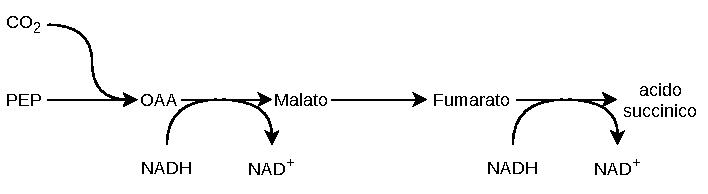
\includegraphics[scale = 0.85]{img/lr1.pdf}
\end{figure}
e si ``ignorano'' gli step intermedi, compattando la rappresentazione,
semplificando le equazioni e la complessità computazionale, ottenendo:
\begin{figure}[H]
  \centering
  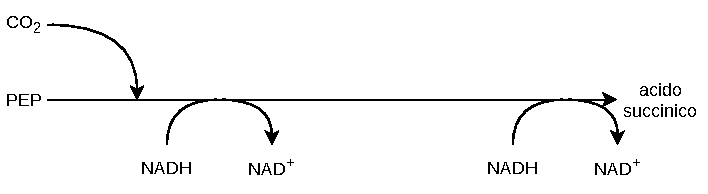
\includegraphics[scale = 0.85]{img/lr2.pdf}
\end{figure}
che presenta quindi, come \textit{steichiometria globale}, solo:
\[-PEP-CO_2-2NADH+Succint\,\,\,Acid+2NAD^{+}=0\]
Per scegliere quindi tra i \textbf{genome wide models} e i \textbf{core models}
si utilizza il principio del \textbf{rasoio di Occam}, cercando di mediare da un
lato per il livello dei dettagli, il costo computazionale, gli errori e gli
eventuali cicli termodinamici infattibili e dall'altro mediando lo studio dello
spazio di fattibilità, la cura manuale del modello, la ``simulabilità'' e la
visualizzazione del modello stesso. Se il processo della costruzione del
\textbf{core model} è ben fatto si ottengono con un centinaio di reazioni
risultati praticamente analoghi a quelli che si avrebbero con 7000 e passa
reazioni.
\subsection{The Enhanced Growth Model}
Studiamo ora, come esempio, il cosiddetto \textbf{The ENhanced GROwth
  (\textit{ENGRO}) model}\footnote{Damiani et al. "A metabolic
  core model elucidates how enhanced utilization of glucose and glutamine, with
  enhanced glutamine-dependent lactate production,
  promotes cancer cell growth: The Warburg
  effect." PLOS Computational Biology 13.9 (2017):
  e1005758.\label{engro1}}.\\
Tale modello, visualizzabile in figura \ref{fig:engro}\footref{engro1},
rappresenta il \textbf{core model}, quindi curato manualmente, di una crescita
migliorata, detta appunto \textit{ENGRO}, che è stato utilizzato per studiare
l'\textit{effetto Warburg}, ovvero la produzione aerobica di lattato dal
glucosio. Tale effetto descrive l'osservazione che le cellule cancerose e molte
cellule cresciute \textit{in vitro} mostrano la fermentazione del glucosio anche
quando è 
presente una quantità sufficiente di ossigeno per respirare adeguatamente. In
altre parole, invece di respirare completamente in presenza di ossigeno
adeguato, le cellule tumorali fermentano. L'\textit{ipotesi di Warburg} era che
l'\textit{effetto 
di Warburg} fosse la causa principale del cancro. L'attuale opinione popolare è
che le cellule cancerose fermentino il glucosio mantenendo lo stesso livello di
respirazione che era presente prima del processo di carcinogenesi, e quindi
l'effetto Warburg sarebbe definito come l'osservazione che le cellule cancerose
mostrano glicolisi con secrezione di lattato e respirazione mitocondriale in
presenza di
ossigeno\footnote{\url{https://it.wikipedia.org/wiki/Ipotesi_di_Warburg}}. 
\begin{figure}
  \centering
  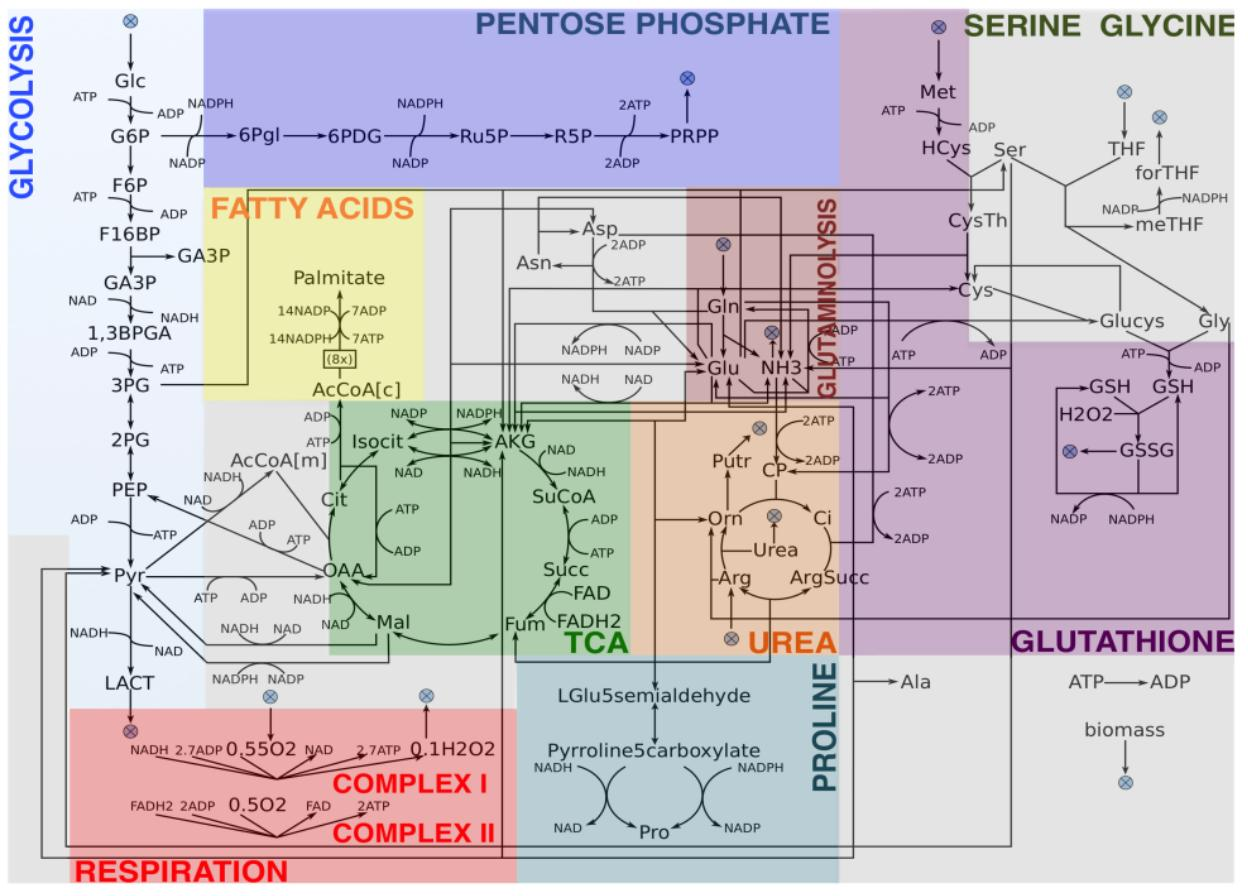
\includegraphics[scale = 0.25]{img/engro.jpg}
  \caption{Rappresentazione dei pathway della mappa metabolica del modello
    \textit{ENGRO}}
  \label{fig:engro}
\end{figure}
Per studiare questo sistema non ci si è limitati ad una singola funzione
obiettivo di programmazione lineare ma se ne sono studiate diverse, avendo di
fatto un \textbf{problema di meta-programmazione}. Si studia quindi tutto il
possibile spazio delle soluzioni della \textit{FBA} nonché come si possa
perturbare un modello e utilizzare ancora la \textit{FBA} per analizzare la
perturbazione.
\subsubsection{Studio delle Multiple Soluzioni}
In primis vengono quindi studiati i possibili risultati che si ottengono con la
\textit{FBA}. Un esempio potrebbe essere quello di voler studiare il tasso di
crescita in funzione della disponibilità di nutrienti in ingresso la sistema e
cercare l'ottimo, notando come al calare del Glucosio si necessita di più
Ossigeno e viceversa.\\
Un primo studio con il modello \textit{ENGRO} è quindi quello di porre
determinati vincoli alle sostanze in ingresso al sistema, ovvero a certi flussi,
e studiare, ottica di una certa funzione obiettivo, la distribuzione ottimale
dei flussi, vedendo quali sono up-regolati e quali down-regolati. \\
Ovviamente le soluzioni ottime possono essere differenti e quindi è bene
esplorare l'intero spazio delle soluzioni accettabili, variando i vari pesi
etc$\ldots$, facendo anche in modo che certe reazioni si abilitino/disabilitino
di volta in volta. Ad esempio si considerino le seguenti condizioni
sull'insieme delle soluzioni e su un numero $j$ di interazioni:
\begin{gather*}
  \sum_{i\in NZ_{j-1}} y_i\geq 1\\
  \sum_{i\in NZ_{j}} w_i\leq |NZ_k|-1,\,\,\forall k = 1,2,\ldots,j-1\\
  y_1+w_i\leq 1,\,\,\forall i\\
  \alpha w_i\leq v_i\leq \beta w_i,\,\,\forall i
\end{gather*}
Ad ogni iterazione $j$ almeno uno dei flussi non nulli provenienti dalla
soluzione precedente, ovvero $NZ_{j-1}$, deve essere impostato a zero, dove la
variabile binaria $y_i$ 
è 1 se quel flusso è selezionato per essere rimosso dalla base all'iterazione
$j$. La variabile binaria $w_i$ viene successivamente forzata a zero se $y_i$ è
uno, e i limiti superiore e inferiore per quel particolare flusso sono quindi
vincolati a zero.\\
Le equazioni assicurano che le basi alternative non vengano rivisitate
eliminando almeno una variabile diversa da zero trovata nelle iterazioni
precedenti. Questo è quindi un algoritmo ricorsivo per il calcolo di ottimi
alternativi utilizzando la \textbf{programmazione lineare intera mista, mixed
integer linear programming (\textit{MILP})} e ci permette di enumerare le varie
soluzioni alternative.
\subsubsection{Studio delle Perturbazioni al Sistema}
Un'altra cosa interessante da studiare è come cambi il \textit{fenotipo} al
variare di determinate perturbazioni al sistema. Si parte quindi con un
\textbf{fenotipo wild-type} e gli si applicano vari cambiamenti al fine di
ottenere un \textbf{fenotipo modificato}. Tra le prime perturbazioni che si
applicano si hanno:
\begin{itemize}
  \item perturbazioni ai nutrienti, che non cambiano la termodinamica del
  sistema 
  \item delezione di geni, ottenendo le vere e proprie mutazioni
\end{itemize}
Inoltre si possono fare altri test, meno frequenti, come:
\begin{itemize}
  \item delezione di reazioni
  \item shock termico, avendo che, essendo le reazioni sensibili alla
  temperatura, si può avere la rottura dell'equilibrio del sistema avendo quindi
  reazioni di tipo diverso da studiare
\end{itemize}
Dal punto di vista più modellistico/matematico si hanno vari modi di studiare la
perturbazione del sistema.\\
Un primo approccio è usare semplicemente la \textit{FBA}, simulando le risposte
metaboliche, ad esempio studiando i \textit{knockout} (che potrebbero essere
multipli nel sistema in analisi) e la variazione di nutrienti. Prendiamo quindi
un esempio dove, nel caso wild-type, vogliamo massimizzare la crescita. Si ha
quindi una certa funzione obiettivo con determinati vincoli, del tipo:
\begin{equation*}
  \begin{array}{rrclcl}
    \displaystyle \max & f_{growth} \\
    \textrm{s.t.} & b_L & \leq & f & \leq b_{U} \\
                       & Sf & = & [0] \\
  \end{array}
\end{equation*}
Usando semplicemente la \textit{FBA} vengono magari aggiunti dei vincoli,
ottenendo:
\begin{equation*}
  \begin{array}{rrclcl}
    \displaystyle \max & f_{growth} \\
    \textrm{s.t.} & b_L & \leq & f & \leq b_{U} \\
                       & Sf & = & [0] \\
                       & b_L & \leq & f_{mut} & \leq b_{U} \\
  \end{array}
\end{equation*}
Dove tali vincoli aggiuntivi magari rappresentano una delle perturbazioni sopra
elencate. \\
Si hanno comunque dei limiti:
\begin{itemize}
  \item la mutazione potrebbe non crescere in modo ottimale se la selezione
  naturale non ha avuto la possibilità di agire sul nuovo background genetico 
  \item si è ``solo'' trovata un'ottimo alternativo, avendo comunque, dal punto
  di vista della programmazione lineare, soluzioni che si trovano sui vertici
\end{itemize}
Questa procedura comunque viene normalmente automatizzata, magari usando una
lista di geni da attivare/disattivare, tenendo traccia di ogni cambiamento e
della variazione di risultati ottenuta tramite esso.\\
Superando l'approccio classico il primo passo è quello di introdurre una
particolare ipotesi biologica, detta \textbf{Minimization of Metabolic
  Adjustment (\textit{MOMA}) hypothesis}, che ipotizza che una mutazione
tenderà ad approssimare quando si ha con il wild-type il più possibile. Più
formalmente viene trovato un vettore di flusso \textit{MOMA} con distanza
euclidea minima da una singola entità wild-type ottimale, soggetta ai vincoli
della mutazione. Si ha quindi una certa funzione obiettivo con determinati vincoli, del tipo:
\begin{equation*}
  \begin{array}{rrclcl}
    \displaystyle \max & f_{growth} \\
    \textrm{s.t.} & b_L & \leq & f & \leq b_{U} \\
                       & Sf & = & [0] \\
  \end{array}
\end{equation*}
e, usando l'ipotesi \textit{MOMA}, si potrebbe arrivare a qualcosa del tipo:
\begin{equation*}
  \begin{array}{rrclcl}
    \displaystyle \min & |m-f_{opt}| \\
    \textrm{s.t.} & b_L & \leq & f & \leq b_{U} \\
                       & Sm & = & [0] \\
                       & b_L & \leq & f_{mut} & \leq b_{U} \\
  \end{array}
\end{equation*}
Ottenendo quindi non un ottimo su un vertice ma la soluzione più vicina, sotto
l'ipotesi \textit{MOMA}. Ovviamente anche in questo caso si hanno delle
limitazioni: 
\begin{itemize}
  \item l'ipotesi \textit{MOMA} spingerà il metabolismo nel mutante verso la
  distribuzione arbitraria di flusso ottimale singola ottenuta con la
  \textit{FBA} ma esistono comunque soluzioni alternative che massimizzano la
  crescita e altre soluzioni sub-ottimali    
  \item la crescita non è comunque assicurata nelle mutazioni
\end{itemize}
Un altro approccio è quello più probabilistico, basato su un \textbf{sampling
  randomico} dei vari parametri di programmazione lineare. In questo caso con:
\begin{equation*}
  \begin{array}{rrclcl}
    \displaystyle \max & f_{growth} \\
    \textrm{s.t.} & b_L & \leq & f & \leq b_{U} \\
                       & Sf & = & [0] \\
  \end{array}
\end{equation*}
Si otterrebbe di volta un volta un certo spazio di soluzioni accettabili per
l'entità wild-type mentre con:
\begin{equation*}
  \begin{array}{rrclcl}
    \displaystyle \min & |m-f_{opt}| \\
    \textrm{s.t.} & b_L & \leq & f & \leq b_{U} \\
                       & Sm & = & [0] \\
                       & b_L & \leq & f_{mut} & \leq b_{U} \\
  \end{array}
\end{equation*}
semplicemente si riduce tale spazio.\\
Si hanno quindi due tipologie di approccio per il \textit{sampling}:
\begin{enumerate}
  \item \textbf{Hit-and-Run (\textit{HR})}, dove si ha \textit{sampling}
  uniforme all'interno della regione delle soluzioni permesse, ovvero un punto
  valido iniziale viene spostato ripetutamente all'interno dello spazio secondo
  regole probabilistiche. Si ottiene quindi\footnote{Bordel et al., PLoS
    Comp. Bio. 2010} una funzione obiettivo del tipo, avendo $i$ e $j$ una
  coppia casuale di reazioni:
  \[F=w_if_i+w_jf_j\]
  \item \textbf{Convex Basis (\textit{CB})} dove si usa l'\textit{algoritmo del
    simplesso} con un insieme casuale di funzioni obiettivo da massimizzare. La
  massimizzazione di ciascuna di queste funzioni obiettivo darà un angolo nello
  spazio delle soluzioni. In pratica in questo caso il \textit{sampling} è solo
  sugli spigoli
\end{enumerate}
Ovviamente il numero di combinazioni che si ottengono con il \textit{sampling}
può essere veramente enorme quindi deve essere effettuato ``sotto controllo''.\\
Un altro elemento interessante è il cosiddetto \textbf{\textit{ENGRO}
  Z-score}\footnote{Damiani et al. ”A metabolic core model elucidates how
  enhanced utilization of glucose and glutamine, with enhanced
  glutamine-dependent lactate production, promotes cancer cell growth: The
  Warburg effect.” PLOS Computational Biology 13.9 (2017): e1005758.}. Tale
valore altro non fa misurare la differenza tra la mutazione e l'entità
wild-type, facendo misure su media del wild-type e deviazione standard:
\[Z=\frac{\overline{X}_1-\overline{X}_2}{\sqrt{\frac{\sigma_1^2}{n}+
      \frac{\sigma_2^2}{n}}}\]
Avendo quindi che un valore alto per $Z$ corrisponde ad un'alta differenza tra
l'entità wild-type e la mutazione.
\subsection{Ricerca di Valori Sub-Ottimali}
Attualmente lo studio tramite i metodi basati sulla \textit{FBA} presenta
diverse limitazioni, anche se alcune estensioni sono possibili per superare
alcune di queste:
\begin{itemize}
  \item si basa sull'assunzione di \textit{steady-state}, comportando difficoltà
  nello studiare la dinamica del sistema
  \item non fornisce alcuna una informazione sulle concentrazioni dei
  metaboliti 
  \item obbliga una scelta limitata della funzione obiettivo
  \item presenta limite nel predire il comportamento netto, ovvero la somma dei
  flussi, di cellule possibilmente eterogenee all'interno di una
  popolazione. Questa è una forte limitazione nel caso dei tumori dove si hanno
  differenti popolazioni e dove non si sa da quale popolazione arrivi una certa
  produzione  
\end{itemize}
Inoltre ci si è chiesti se il metabolismo funzioni unicamente per massimizzare
il tasso di crescita. Si hanno evidenze, studiate in
laboratorio\footnote{Fischer, Nat Genet 2005} su \textit{Bacillus subtilis}, un
batterio, che la delezione di alcuni geni metabolici causano un aumento dei
tassi di crescita e della resa di biomassa rispetto all'entità wild-type. La
pressione selettiva per aumentare il tasso di crescita deve essere bilanciata da
altre richieste sul metabolismo, come il mantenimento cellulare o l'apparato
sensoriale, riducendo il tasso di crescita a favore della forma fisica
complessiva. Come detto questo si è studiato in laboratorio ma nulla assicura
che la crescita legata alla delezione di alcuni geni possa avvenire anche in
natura in quanto magari quel gene codificava per qualche aspetto che era
vantaggioso ad altri aspetti della sopravvivenza e senza non si ha possibilità
di sopravvivere. Inoltre le limitazioni del tempo evolutivo e della variabilità
genetica possono significare che il metabolismo non è ottimale per nessun
obiettivo, quindi non possiamo necessariamente escludere dalla considerazione
le molte configurazioni di flusso che supportano, ad esempio, il 90\% (ma anche
percentuali) di crescita massima. Queste configurazioni di supporto tornano
comodo in fase di decisione dei vincoli di programmazione lineare.\\
Il punto chiave del discorso è che magari con una soluzione ottima dal punto di
vista del tasso di crescita si porta a massimizzare la biomassa mentre con una
soluzione sub-ottimale, sempre lato tasso di crescita, si ottiene non solo una
biomassa accettabile ma magari anche, per esempio, la produzione di altri
componenti, magari biocarburanti. \\
Partendo quindi dalla classica:
\begin{equation*}
  \begin{array}{rrclcl}
    \displaystyle \max & f_{growth} \\
    \textrm{s.t.} & b_L & \leq & f & \leq & b_{U} \\
                       & Sf & = & [0] \\
  \end{array}
\end{equation*}
Si hanno tre alternative:
\begin{enumerate}
  \item aggiungere vincoli, lavorando come già visto con la \textit{FBA}
  classica, ottenendo una soluzione sub-ottimale che però comporta anche qualche
  produzione aggiuntiva (come nell'esempio ipotetico quella di biocarburanti)
  \item vincolare la biomassa ed esplorare lo spazio della soluzione risultante
  tramite sampling dello spazio delle soluzioni, avendo quindi, con una
  configurazione di supporto che porta la biomassa al 90\%:
  \begin{equation*}
    \begin{array}{rrclcl}
      \displaystyle sampling\\
      \textrm{s.t.} & b_L & \leq & f\,\,\,\,  \leq b_{U} \\
                    & Sf & = & [0] \\
                    & f_{biomass} & \leq & 0.9 \cdot  OPT_{biomass} 
    \end{array}
  \end{equation*}
  Si ha quindi una soglia per il livello minimo di biomassa accertabile,
  nell'esempio il 90\% della biomassa dell'entità wild-type, e si ha
  come risultato un insieme di soluzioni e non una singola soluzione
  \item usare una funzione obiettivo multi-pesata, cambiando quindi la forma
  stessa della funzione. Si ottiene, ad esempio una cosa del tipo:
  \begin{equation*}
    \begin{array}{rrclcl}
      \displaystyle \max & f_{MW} \\
      \textrm{s.t.} & b_L & \leq & f\,\,\,\,  \leq b_{U} \\
                         & Sf & = & [0] \\
                         & f_{biomass} & \leq & 0.9 \cdot  OPT_{biomass} \\
    \end{array}
  \end{equation*}
  dove la funzione obiettivo multi-peso, $f_{MW}$ è, ad esempio, del tipo:
  \[f_{MW}=0.8f_{G}  +  0.1f_F +  0.1f_I\]
  Quindi non si massimizza il 100\% della biomassa ma un certo $(100-x)$\%,
  avendo quindi che il sub-ottimo della biomassa viene comunque cercato in uno
  spigolo, e distribuendo quella percentuale residua $x$ ad altre reazioni
\end{enumerate}
\subsection{Metabolic Rewiring}
Si torna quindi a parlare di cancro.\\
Possiamo vedere il cancro come una ``malattia stocastica'', risultante da una
serie di mutazioni che colpiscono le cellule del nostro corpo e comportante la
selezione di un fenotipo utile unicamente ai propri scopi. Le cellule
cancerogene sono quindi, all'incirca, parte di insiemi di cellule normali
che hanno accumulato una serie casuale di mutazioni e modificazioni
epigenetiche. Si ha quindi che l'evoluzione cellulare è stata in questi casi in
qualche modo modificata e quindi possiamo studiare il normale funzionamento del
metabolismo, questa sorta di ``metabolic wiring'' (``collegamento metabolico'')
di 
quegli insiemi che presentano generiche proprietà che corrispondono
statisticamente a quelle delle cellule nella realtà. In termini più matematici
riconosciamo l'area di fattibilità tramite programmazione lineare. All'esterno
di tale area si hanno i fenotipi impossibili mentre all'interno si ha l'insieme
dei fenotipi possibili, insieme in cui si possono riconoscere vari sottoinsiemi
caratterizzati da una proprietà simile (che ha un corrispettivo reale nelle
cellula). Si assume quindi un metabolismo simile tra cellule normali e
cancerogene ma se ne fa uno studio diverso tramite la \textit{FBA}.\\
Per esplorare lo spazio dei possibili ``collegamenti'' si procede tramite
\textit{sampling} causale dei pesi, cambiando quindi funzione obiettivo ogni
volta, e facendo anche \textit{sampling} delle reazioni, puntando infine a
massimizzare la somma pesata dei flussi attraverso determinate reazioni. Le
distribuzioni di flusso ottenute possono essere una rappresentazione efficiente
di una popolazione cellulare mutata casualmente, ad esempio l'attivazione
mutata di un gene che codifica per un enzima metabolico corrisponderebbe a
un tentativo di aumentare il flusso attraverso quell'enzima. \\
Dopo aver fatto varie analisi tramite la \textit{FBA} si creano insiemi di
diverse risposte metaboliche alle perturbazioni e si procede creando una sorta
di albero binario, che si dirama in base alle percentuali di riuscita di
determinate azioni. Da tale albero si possono poi ottenere diverse informazioni
sul sistema, in quanto le diverse diramazioni permettono di distinguere il
comportamento normale da quello cancerogeno.\\
Tutte queste analisi sono ora usate anche in ambito \textit{single-cell}.
\chapter{Progressione Tumorale}
Si introduce ora in modo più dettagliato lo studio della \textbf{progressione
  tumorale} e della modellazione della stessa. Si parla quindi dell'analisi dei
dati relativi a tumori con una gran varietà di fini, tra cui la \textit{medicina
  traslazionale}. Si introducono quindi una serie di tecniche e tecnologie atte
al ricostruire possibili modalità/sequenze relative alla progressione
tumorale (introducendo anche qualche lavoro fatto in \textit{DCB}, ex
\textit{BIMIB}, in \textit{Bicocca}, fatti i collaborazione con molti altri
atenei sparsi nel mondo, da quello di \textit{UCLA} a quello di
\textit{Trieste}).
\section{Approfondimento Biologico}
Prima di parlare di vera e propria modellistica bisogna introdurre alcuni
concetti biologici essenziali.\\
Riprendendo la figura \ref{fig:cp} possiamo riconoscere i vari step della
progressione, arrivando fino ad un \textbf{adenoma}, ovvero un cosiddetto
\textit{polipo intestinale} e al \textbf{carcinoma} e questo è visualizzabile
ancora meglio, in modo meno srtilizzato anche se manca la rappresentazione della
\textbf{metastasi}, in figura \ref{fig:cp2}\footnote{Batlle E. et al. Nat Genet,
  39, 1376-83 (2007)}, ovvero nel dettaglio del \textbf{Colon Rectal Cancer
  (\textit{CRC})}. Come detto le modalità di progressione sono molteplici e
lo studio delle stesse è centrale nel discorso della cosiddetta \textbf{medicina
  personalizzata}.  
\begin{figure}
  \centering
  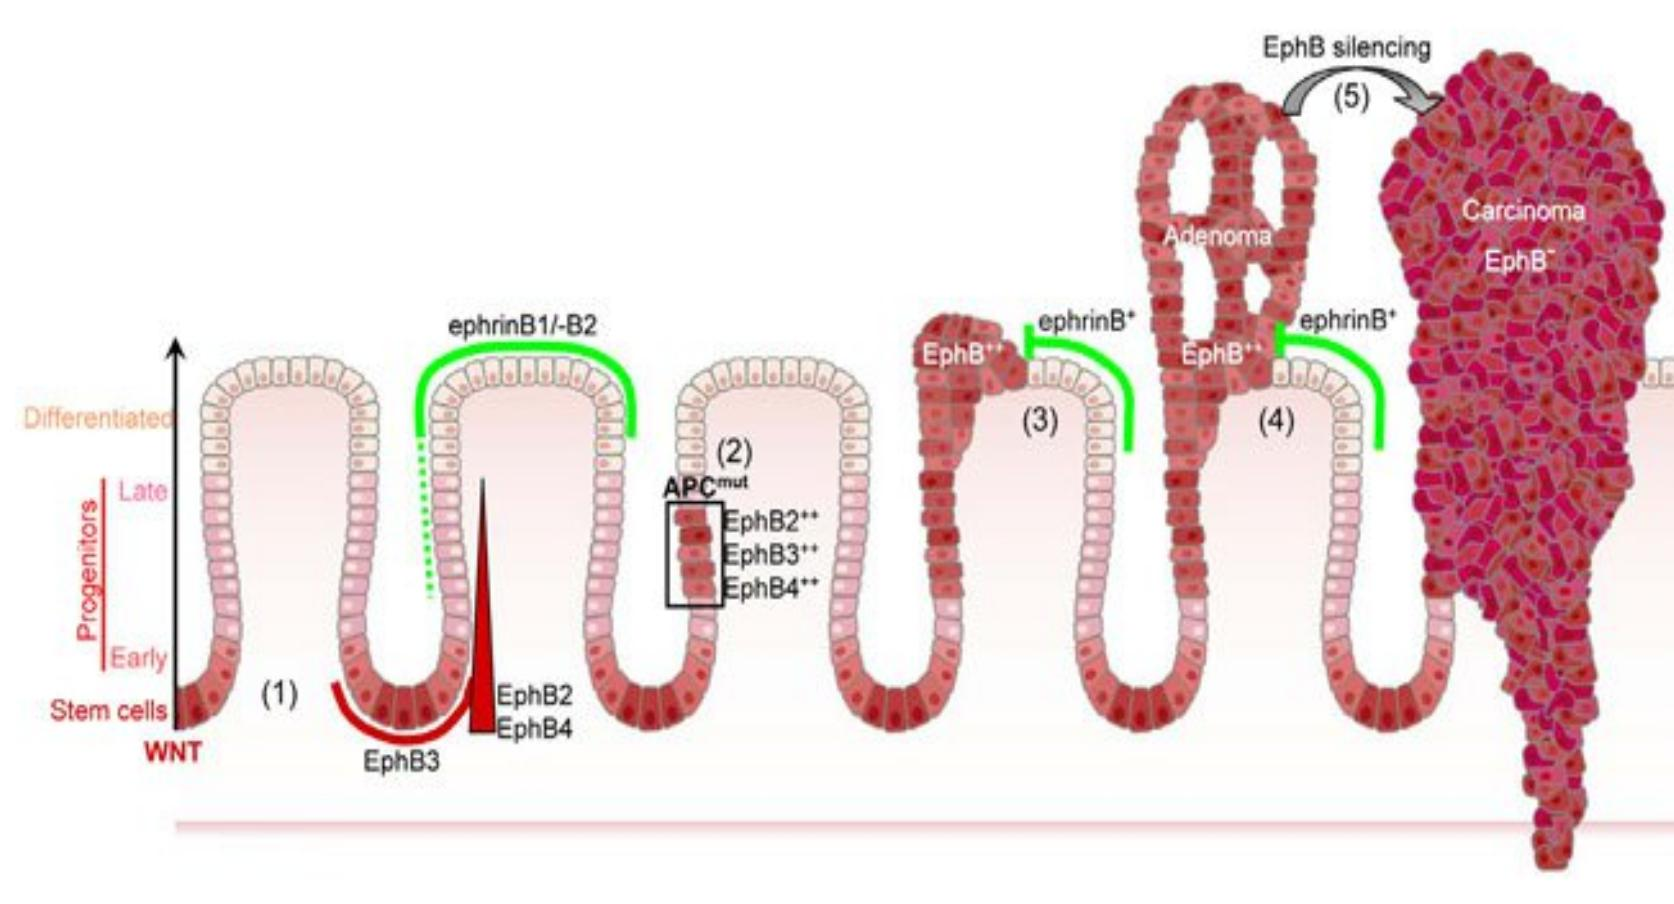
\includegraphics[scale = 0.2]{img/cp2.jpg}
  \caption{Rappresentazione meno schematica di uno dei modelli di progressione
    tumorale del cancro.}  
  \label{fig:cp2}
\end{figure}
Sempre parlando di \textit{CRC} bisogna anche introdurre il concetto di
\textbf{staging}
\footnote{\url{https://www.cancer.net/cancer-types/colorectal-cancer/stages}}.
La progressione del tumore avviene infatti in vari step, nel 
dettaglio del \textit{CRC} se ne individuano tendenzialmente quattro, che
portano dallo stato iniziale allo sviluppo ormai incontrollato e di
\textit{metastasi} del tumore anche in altri organi. Un esempio è lo
\textit{stage 3}, dove si hanno giù più tumori all'interno del colon, tumori che
si scoprono tramite \textit{colonscopia}, avendo quindi una \textbf{metastasi
  locale} ma non avendo comunque la \textbf{metastasi distante}, ovvero che
ormai ha raggiunto anche altri organi. In questo contesto è anche interessante
lo studio delle immagini, sia tramite una commissione di tre dottori che
stabiliscono l'entità della progressione tumorale, che, in modo più
computazionale, tramite modelli di \textit{machine learning} e tecniche di
\textit{intelligenza artificiale} per l'analisi di immagini.\\
Si deve quindi studiare la progressione della malattia e una buona ipotesi sulla
maggior parte dei tipi di cancro è che il disturbo progredisce attraverso
fasi/stage accumulando alterazioni che influenzano la funzione e le interazioni
dei geni. Ad ogni step quindi si accumulano mutazioni etc$\ldots$. Si giunge
quindi ad alcune conclusioni:
\begin{itemize}
  \item il malfunzionamento di singoli geni non può, da un certo di vista
  purtroppo, causare il cancro. Questa è stata una speranza anni fa in quanto
  avrebbe semplificato di gran lunga lo studio di cure per i vari tumori mentre
  si è arrivati a capire che un tumore deriva da multipli malfunzionamenti di
  multipli geni
  \item il cancro si sviluppa attraverso multipli percorsi evolutivi, essendo
  quindi un problema capire dove effettivamente si sviluppa il tumore, avendo
  che questo aspetto dipende dai nutrienti etc$\ldots$
  \item le alterazioni si possono categorizzare in vari modi, ma tra i
  principali si hanno:
  \begin{itemize}
    \item \textbf{mutazioni somatiche}. Una \textit{mutazione somatica} è una
    mutazione a livello del DNA di una qualunque cellula del corpo (cellule
    somatiche) eccezion fatta quindi per le cellule della linea germinale;
    pertanto essa non viene trasmessa alla discendenza. Nel caso in cui
    l'elemento colpito sia una cellula ancora in grado di dividersi la mutazione
    viene trasmessa a tutte le cellule che derivano da essa per
    \textit{mitosi}. In questo caso l'organismo diviene un mosaico cioè sara'
    costituito da una popolazione di cellule normali ed una di cellule
    mutate\footnote{\url{https://www.molecularlab.it/principi/dizionario/
        definizione.asp?w=Mutazione\%20somatica}}
    \item \textbf{Copy number variation (\textit{CNV})}, ovvero il fenomeno in
    cui si ripetono sezioni del genoma e il numero di ripetizioni nel genoma
    varia da individuo a individuo. La variazione del numero di copie è un tipo
    di variazione strutturale: nello specifico, è un tipo di evento di
    duplicazione o cancellazione che interessa un numero considerevole di coppie
    di basi, comportando ad esempio \textit{over-espressione} (ma anche
    l'opposto) di certe proteine, con conseguenze non sempre
    positive\footnote{\url{https://en.wikipedia.org/wiki/Copy_number_variation}}
  \end{itemize}
  Questi, e molti altri, eventi sono dovuti, ad esempio, dal
  \textit{microambiente} etc$\ldots$, avendo che le cause per la progressione
  del tumore possono essere davvero molteplici
\end{itemize}
Come detto quindi tutto questo studio di modellazione è essenziale per lo
sviluppo di farmaco e per decisioni terapeutiche, ad esempio, è noto che per lo
stesso tipo di cancro, i pazienti in diverse fasi/stage di diverse progressioni
rispondono in modo diverso a diversi trattamenti. Un certo stadio richiede
infatti un certo dosaggio di \textit{chemioterapia} a differenza di un altro,
avendo quindi che la \textit{quantificazione della terapia} è essenziale in
questo contesto medico.\\
Le cellule cancerogene sono come le altre cellule, da un certo punto di vista, e
possono quindi essere studiate come dei \textit{replicatori individuali}. Lo
scopo è comunque quello di \textbf{riprodursi/replicarsi} e per questo fine tali
cellule, ma come quelle normali del resto, devono fare tre cose:
\begin{enumerate}
  \item \textit{crescere}, attraverso il consumo di energia e tramite i
  nutrienti etc$\ldots$
  \item \textit{vivere a lungo}, nonché \textit{prosperare}, e per questo devono
  limitare/evitare l'\textit{apoptosi}
  \item \textit{muoversi}, e nel caso delle cellule cancerogene questo avviene
  tramite la \textbf{metastasi}
\end{enumerate}
Una cellula cancerosa è quindi essenzialmente una cellula che ha scambiato, a
causa di una molteplicità di fattori, una
serie di comportamenti, dettati dal suo corredo genetico, per altri, più ``di
successo'' nel suo microambiente, sfortunatamente il concetto di ``più di
successo'' per la cellula è un problema per l'organismo. Si avvicina quindi
l'evoluzione tumorale a quanto studiato da Darwin in merito alla
\textbf{selezione naturale}. Riuscendo a replicarsi, queste cellule danno
origine a una nuova popolazione \textit{(sub)clonale} che continua ad
espandersi, generando così una \textit{crescita neoplastica}, ovvero la crescita
anormale delle cellule che porta poi al tumore, avendo quindi una
\textit{crescita cancerogena}. \\
Negli anni, tra le cause di tumori, si sono scoperte anche le cause sterne. In
Giappone, anni fa, è stato fatto infatti un esperimento in cui si usava del
catrame per ``dipingere'' le orecchie di alcuni conigli scoprendo che di
conseguenza si aveva la formazione di tumori proprio in quelle zone. Questo
aspetto aggiunge ulteriore complessità ai vari studi.\\
Bisogna quindi ora cpire quali siano i ``segni distintivi'' del cancro, i
cosiddetti \textbf{cancer hallmarks}\footnote{Hanahan D, Weinberg RA. The
  hallmarks of cancer. Cell. 2000 Jan 7;100(1):57-70. doi:
  10.1016/s0092-8674(00)81683-9. PMID: 10647931.}. Tali \textit{hallmarks} di
tale ``nuovo'' modo di funzionamento, ovvero quello cancerogeno, conferendo alle
cellule tumorali forme di vantaggio selettivo, sono stati descritti come segue:
\begin{itemize}
  \item autosufficienza dal punto di vista dei \textit{segnali dei crescita},
  ricordando che a livello cellulare i \textit{segnali} sono ricevuti dalle
  cellule tramite le proteine
  \item insensibilità ai segnali anti-crescita che cercano di limitare la
  crescita tumorale incontrollata
  \item evitare la morte cellulare programmata, evitando l'\textit{apoptosi}
  segnalata da \textit{p53}
  \item cercare di raggiungere un potenziale replicativo illimitato 
  \item fare angiogenesi, ovvero il processo che porta alla formazione di nuovi
  vasi sanguigni da altri vasi preesistenti, sostenuta. In questo modo si
  comunica al sistema circolatorio di creare vasi sanguigni nei pressi del
  tumore in modo da rifornire meglio nutrienti etc$\ldots$ e favorire la
  crescita incontrollata 
  \item procedere con l'invasione tissutale e la metastasi
  \item deregolamentare il metabolismo (ed è quanto si studia con la
  \textit{FBA})
  \item eludere il sistema immunitario, che non reagisce solo con l'apoptosi ma
  anche con molte altre operazioni
  \item portare all'instabilità del genoma 
\end{itemize}
Tutti questi comportamenti estremizzano i comportamenti che comunque avrebbe
ogni cellula per ottenere le tre cose elencate sopra, necessarie alla
replicazione: crescere, vivere a lungo e muoversi. \\
Sempre in merito al confronto con Darwin possiamo notare come si parta,
nell'evoluzione tumorale, con una certa cellula, staminale o progenitrice, in un
certo microambiente, che si divide, accumulando nei vari microambienti varie
mutazioni e creando la situazione tumorale. Un processo analogo, \textbf{ad
  albero}, è quello che Darwin ha osservato per lo studio
dell'\textit{evoluzione delle specie}. Un \textit{clone}, nel contesto tumorale,
arriva e sopravvive quando è ``migliore'' delle cellule normali e degli altri
cloni, arrivando alla fine, eventualmente, ad avere solo cloni.
\section{Studio della Progressione}
Indicativamente ormai lo studio di queste problematiche avviene tramite la
creazione di grafici, come in figura \ref{fig:gra1}\footnote{A. Fischer et al.,
  High-Definition Reconstruction of Clonal Composition in Cancer, Cell Reports
  7, 2014}, in cui
comunque si parte dai dati prodotti dal \textit{sequenziamento}. I dati hanno
comunque spesso problemi:
\begin{itemize}
  \item dati mancanti, per varie motivazioni tecniche
  \item mancanza di \textit{time point} utili. Si hanno infatti spesso
  \textit{time point} molto distanti e con distanze non uniformi e crescenti,
  dovuti principalmente al modo in cui i biologi vogliono/possono fare le
  sperimentazioni in laboratorio (magari all'inizio si hanno check ogni due
  giorni, poi ogni quattro etc$\ldots$)
\end{itemize}
\begin{figure}
  \centering
  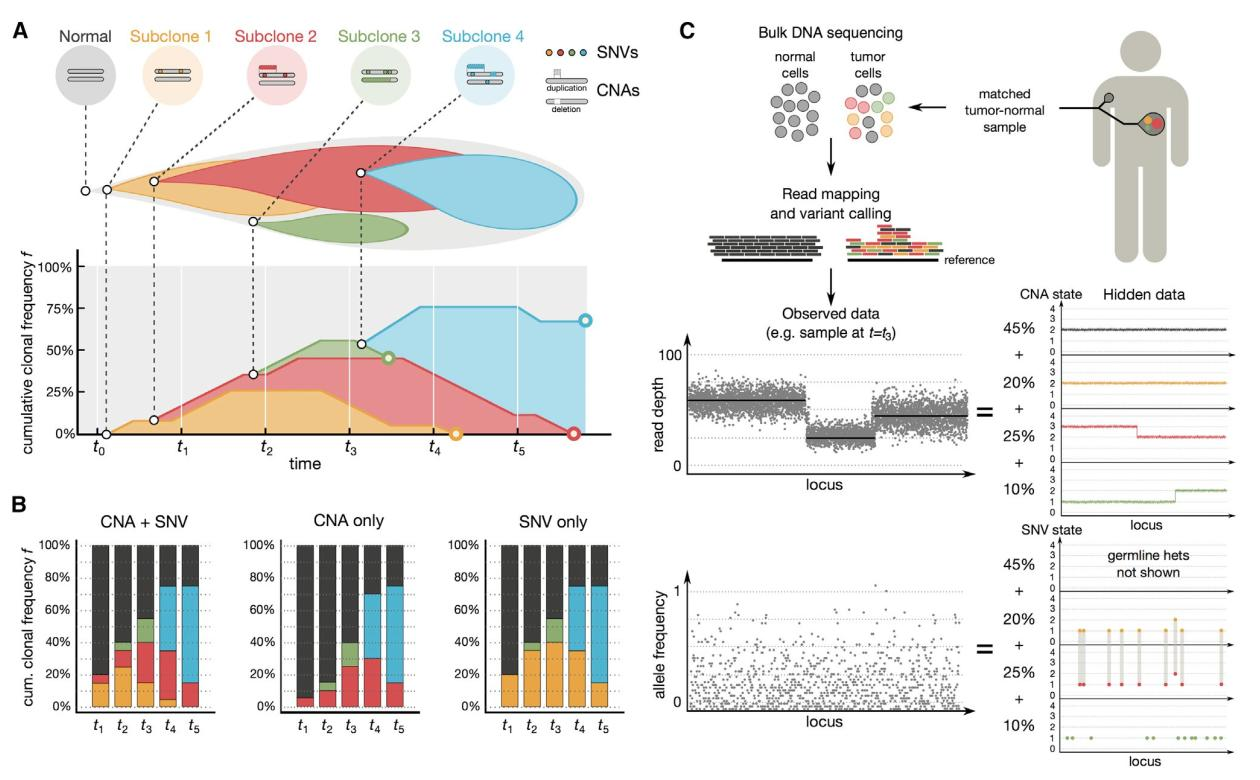
\includegraphics[scale = 0.28]{img/gra1.jpg}
  \caption{Esempio di grafici ottenuti dai dati durante uno studio di
    progressione tumorale, dove \textit{SNV} sta per \textit{single nucleotide
      variation} mentre \textit{CNA} per \textit{copy number alterations}.}
  \label{fig:gra1}
\end{figure}
Si possono anche avere grafici manuali (\textbf{esempi alla slide 17 della
  lezione 9}), anche se ormai è più raro. \\
In generale tali studi possono anche essere utili, con i giusti \textit{time
  point}, per capire se la \textit{chemioterapia} ha avuto effetto, infatti
alcuni ceppi potrebbero sopravvivere al trattamento e potrebbero riportare alla
formazione del cancro. \\
Un'altro aspetto interessante è la \textbf{Inter-Tumor and Intra-Tumor
  Heterogeneity (\textit{ITH})}, che è stata già introdotta. La \textit{ITH},
per vari discorsi, è comunque une tematica difficile da trattare e
studiare. All'interno di un tumore nello stesso paziente si hanno delle
variazioni, come le \textit{eterogeneità spaziali} (ora molto studiate) e le
\textit{eterogeneità clonali}, ma si hanno anche
variazioni tra lo stesso tumore in diversi pazienti, avendo quindi fare
sfaccettature di \textit{eterogeneità}.  
\subsection{Filogenesi}
Come già introdotto nel corso di bioinformatica si ha il concetto di
\textbf{filogenesi}. Date le tecnologie NGS è ora possibile eseguire progetti di
sequenziamento che rivelano diversi aspetti di un fenomeno biologico, in primis
il cancro.\\
In generale si ha la seguente definizione:
\begin{definizione}
  Definiamo \textbf{filogenesi}, o \textbf{albero filogenetico}, come un albero
  che descrive le sequenze di eventi di speciazione che hanno portato alle
  specie attuali, rappresentate nelle foglie di questo albero. I nodi interni
  non rappresentano specie viventi.
\end{definizione}
In realtà questa definizione, nello studio dalle sequenze alle informazioni
sulle mutazioni nel cancro, può assumere delle varianti\footnote{The evolution
  of tumour phylogenetics: principles and practice, R. Schwartz and
  A. A. Schäffer, Nature Review Genetics, 2017}:
\begin{itemize}
  \item parlando di analisi \textit{cross-sectional}, in ambito di
  \textit{oncogenetica}, si ha un primo studio \textit{inter-patient}, ovvero
  studiando più pazienti. In questo caso si possono studiare varie tipologie di
  cancro, partendo da un probabile progenitore plausibile, che sarà la radice
  dell'albero di filogenesi e arrivando ad identificare vari sottotipi di
  tumore, provenienti dai vari pazienti:
  \begin{figure}[H]
    \centering
    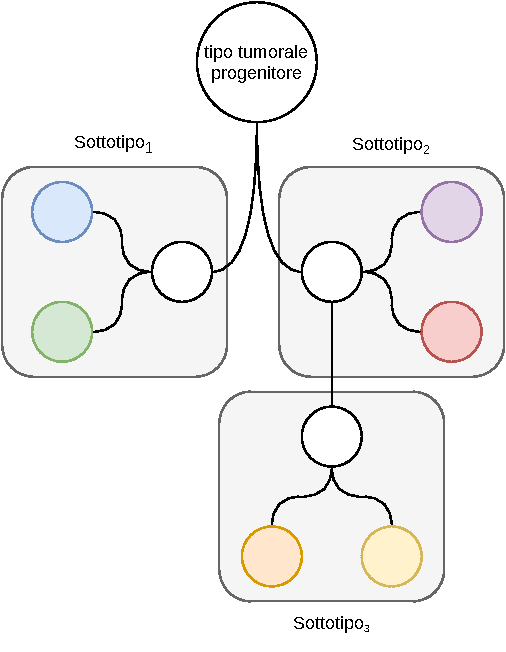
\includegraphics[scale = 0.7]{img/filo1.pdf}
  \end{figure}
  Tali dati sono disponibili nelle varie banche dati, tra cui il \textit{The
    Cancer Genome Atlas} 
  \item parlando di analisi \textit{regional bulk}, tornando a parlare
  dell'individuo singolo e non di una molteplicità di pazienti, si può
  sequenziare un numero 
  di cellule prelevate da un singolo tumore, facendo slice di tessuto tumorale,
  facendo poi \textit{bulk sequencing}. In realtà tale analisi si fa
  usando slice di più tumori relativi a tumori ormai in metastasi in diversi
  organi. Si arriva quindi a creare un albero che studia l'evoluzione interna
  del tumore, studiando i vari tumori primari e metastasi derivanti dal
  progenitore: 
  \begin{figure}[H]
    \centering
    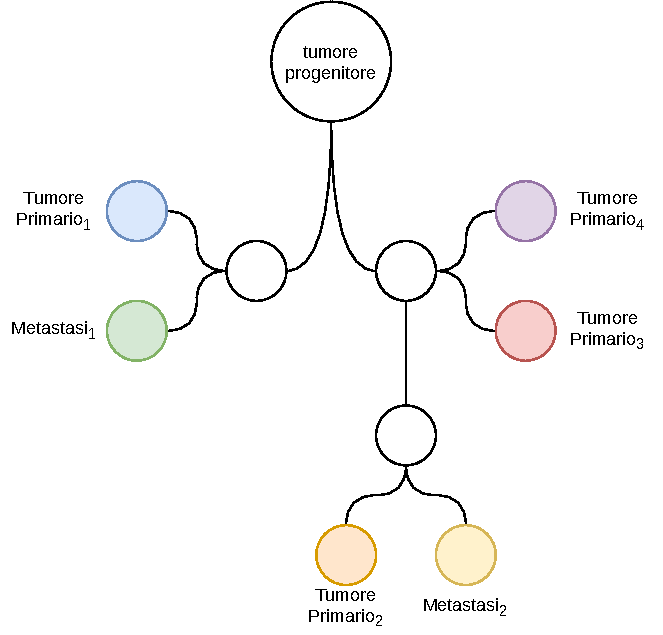
\includegraphics[scale = 0.7]{img/filo2.pdf}
  \end{figure}
  \item parlando di analisi \textit{single-cell}, schematizzata in figura
  \ref{fig:sca}\footnote{Single-cell genome sequencing: current state of the
    science, Charles Gawad, Winston Koh \& Stephen R. Quake, Nature Reviews
    Genetics 17, 175–188 (2016) doi:10.1038/nrg.2015.16} si ha uno studio in
  merito all'isolamento di singole cellule, producendo una \textit{filogenesi}
  dei sub-cloni tumorali:
  \begin{figure}[H]
    \centering
    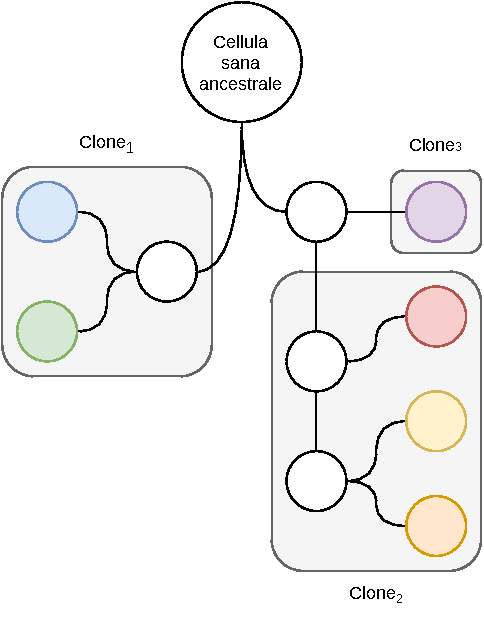
\includegraphics[scale = 0.7]{img/filo3.pdf}
  \end{figure}
  Come sappiamo questa è una tecnica innovativa, ad alta precisione non avendo
  da gestire una moltitudine di ``rumori'' ma avendo un segnale
  individuale. Ogni cellula però deve essere sequenziata più volte, portando ad
  un forte costo (nonostante il singolo sequenziamento ormai sia
  economico). Bisogna quindi cercare il \textit{tradeoff} migliore tra costi e
  qualità.
\end{itemize}
\begin{figure}
  \centering
  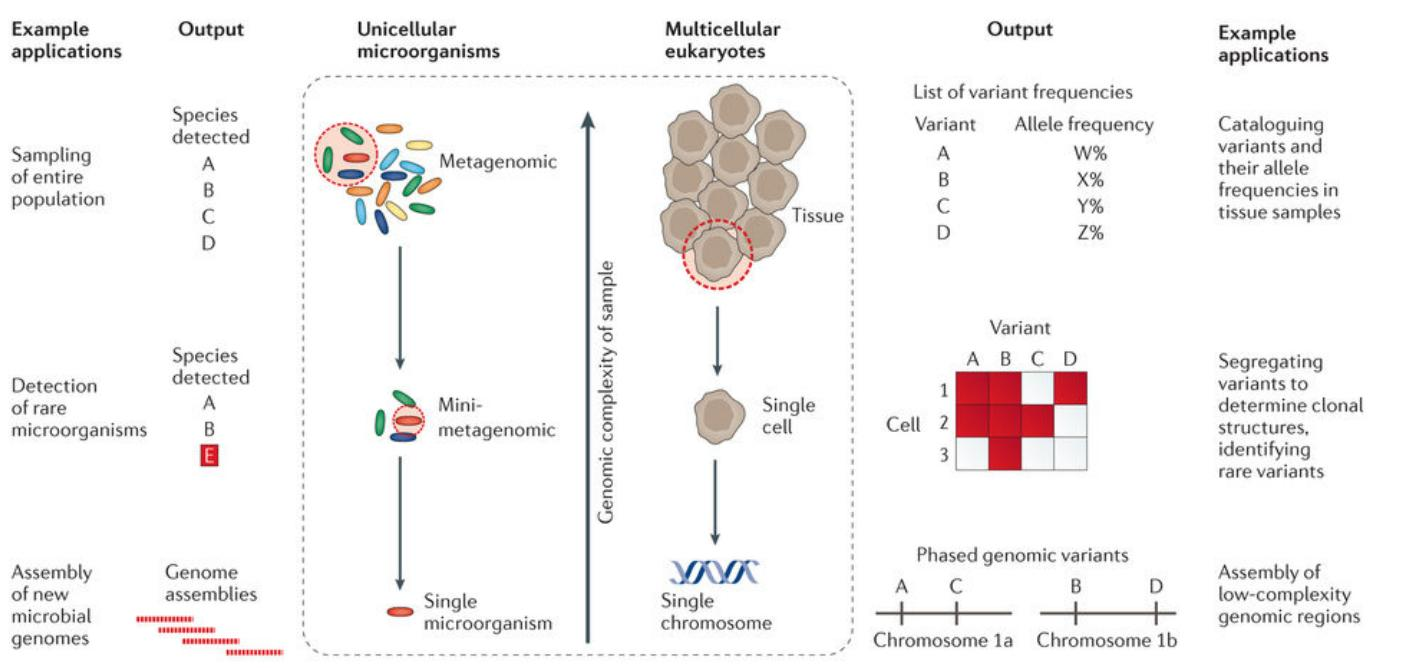
\includegraphics[scale = 0.25]{img/sca.jpg}
  \caption{Schema riassuntivo di funzionamento della \textit{single-cell
      analysis}.} 
  \label{fig:sca}
\end{figure}
\subsection{Cross Sectional Data}
Si approfondisce velocemente la tematica della raccolta dati. Si hanno due
modalità di studio, due livelli:
\begin{enumerate}
  \item \textit{ensemble-level}, dove si cerca di ricostruire un insieme di
  relazioni 
  di precedenza plausibili di eventi a partire da dati dei pazienti, che
  possono essere anche molti. Questo si fa partendo da $n$ dati
  \textit{cross-sectional} indipendenti. Possiamo immaginare di avere una
  matrice con $n$ genomi dei pazienti per le colonne e $m$ ``eventi
  conduttori''. Si ha che $n>m$. Si studiando quindi \textit{SNV} e
  \textit{CNA}, studiando un albero di filogenesi che approfondisce la selezione
  e l'eterogeneità
  \item \textit{individual-level}, dove si cerca di ricostruire un ceppo di
  popolazione di cellule tumorali a partire dal prelievo di tessuto tumorale,
  tramite tecniche filogenesi e single-cell. In questo caso si parte da $n$
  campioni dello stesso tumore, ottenuti da una \textit{biopsia}, e si sequenzia
  tramite \textit{bulk sequencing}. Si ottiene quindi l'albero evolutivo di un
  singolo tumore e si studiano il tumore ancestrale e i cloni senza
  generalizzare la selezione, studiando in modo specifico per il singolo
  paziente 
\end{enumerate}
Si approfondisce quindi l'\textit{ensemble-level}, tramite i
\textit{cross-sectional data}, che rappresentano la maggior parte dei dati
tumorali disponibili, di contro si hanno pochi dati ``longitudinali''. \\
Tali dati sono raccolti da biopsie al momento della diagnosi e, in altre parole,
sono dati di insieme, con pochi ``follow-up'', e ``time-stamp'' (spesso magari
raccolti ma non resi disponibili). Tutti questi dati insieme devono essere
``riordinati'' per ottenere qualche risultato sull'evoluzione tumorale. Dedurre
informazioni temporali da tali dati è una sfida aperta (e non solo parlando di
cancro ma parlando in generale) e il problema è stato
studiato in diversi campi e nel contesto della ricerca sul cancro dalla fine
degli anni '90. Tali dati sono inoltre molto ``rumorosi'' e spesso vengono
gestiti con tecniche di \textit{machine learning} e \textit{reti
  neurali}. Un altro aspetto fondamentale da considerare è quello dei
\textit{dati mancanti}, che complica ulteriormente il discorso.\\
Esempio di analisi in figura \ref{fig:csd}.\\
La gestione di tali dati è comunque un lavoro computazionale e
si hanno le varie banche dati, come \textit{The Cancer Genome Atlas} con vari
portali per accedere semplicemente, tra cui \textit{cBIO portal} o \textit{TCGA
  data portal}. Un altra banca dati è \textit{Firehose}, accessibile tramite
\textit{FireBrowse}. 
\begin{figure}
  \centering
  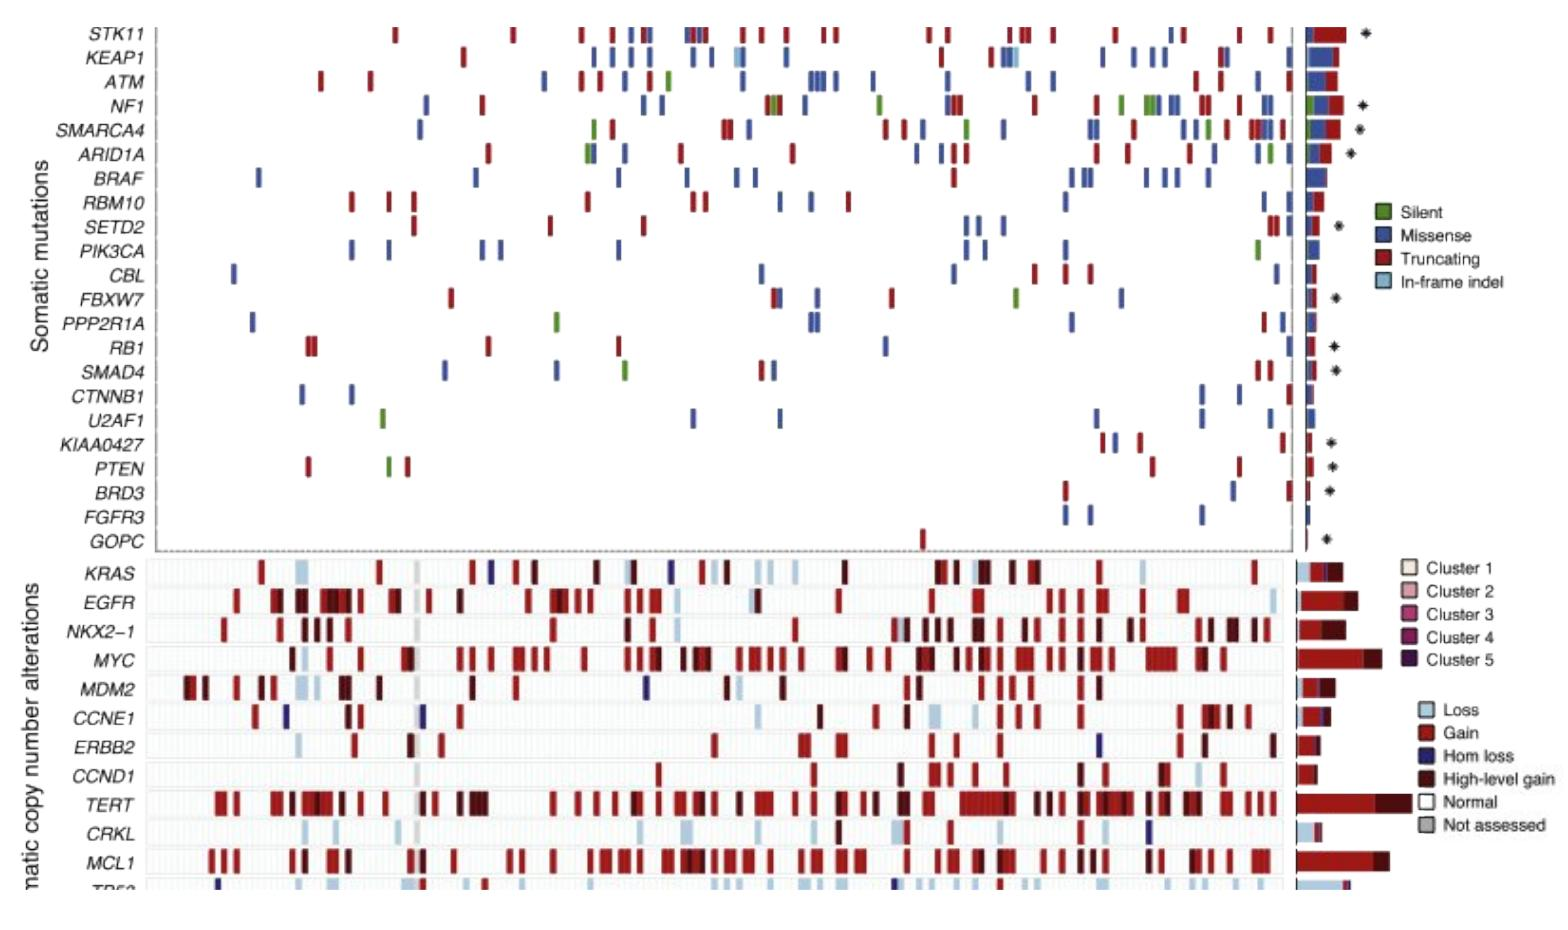
\includegraphics[scale = 0.23]{img/csd.jpg}
  \caption{Esempio di analisi di mutazioni somatiche e \textit{CNA}, nelle due
    parti dell'immagine. Ogni colonna rappresenta un paziente. } 
  \label{fig:csd}
\end{figure}
\subsection{Tipologie di Studio}
A questo punto si vorrebbe rispondere a tre domande:
\begin{enumerate}
  \item possiamo ricostruire un modello di progressione da
  \textit{cross-sectional data}?
  \item cosa è effettivamente contenuto negli insiemi di cosa è effettivamente
  contenuto nella sezione trasversale, essendo ormai cambiati molto negli anni?
  \item che tipo di modelli possiamo ricostruire?
\end{enumerate}
Si vede ora quindi come ricostruire modelli di progressione  per un insieme di
dati, cioè per dati provenienti da più pazienti, usando dei \textbf{Direct
  Acyclic Graph (\textit{DAG})}, che codificano l'accumularsi delle alterazioni
e delle mutazioni, restando quindi sempre in ottica di \textit{dati
  cross-sectional}. \\ 
Una libreria utile in questo contesto è \textit{TRONCO}, sviluppata per
l'ambiente \textit{R}, che contiene varie tecniche ed algoritmi per la
ricostruzione di modelli di progressione.
\subsubsection{Primo Quesito}
Rispondendo al primo quesito si ha quindi una risposta affermativa, avendo
questo schema indicativo, come in figura \ref{fig:q1}\footnote{adattato da:
  Gerstung et al., PLoS ONE, 6(11), 2011}: 
\begin{itemize}
  \item si parte da una matrice booleana dove le colonne sono le mutazioni e le
  righe i tumori, indicando con 1 e 0 la presenza o meno di una certa mutazione
  in un certo tumore
  \item si crea una rete causale, inferita dalla matrice, dove si specifica
  quale mutazione causa. Si ottiene quindi un concetto di ``precedenza''
  \item dalla rete si studia quindi la causalità reciproca tra le mutazioni
  \item dai risultati si studia la causalità a livello di pathway o si studiano
  i fenotipi, ovvero gli \textit{hallmark}, avendo quindi livelli ulteriroi di
  astrazione a partire dal generico \textit{DAG}
\end{itemize}
A partire da questo tipo di modelli si possono ottenere le corrette terapie per
curare un paziente.
\begin{figure}
  \centering
  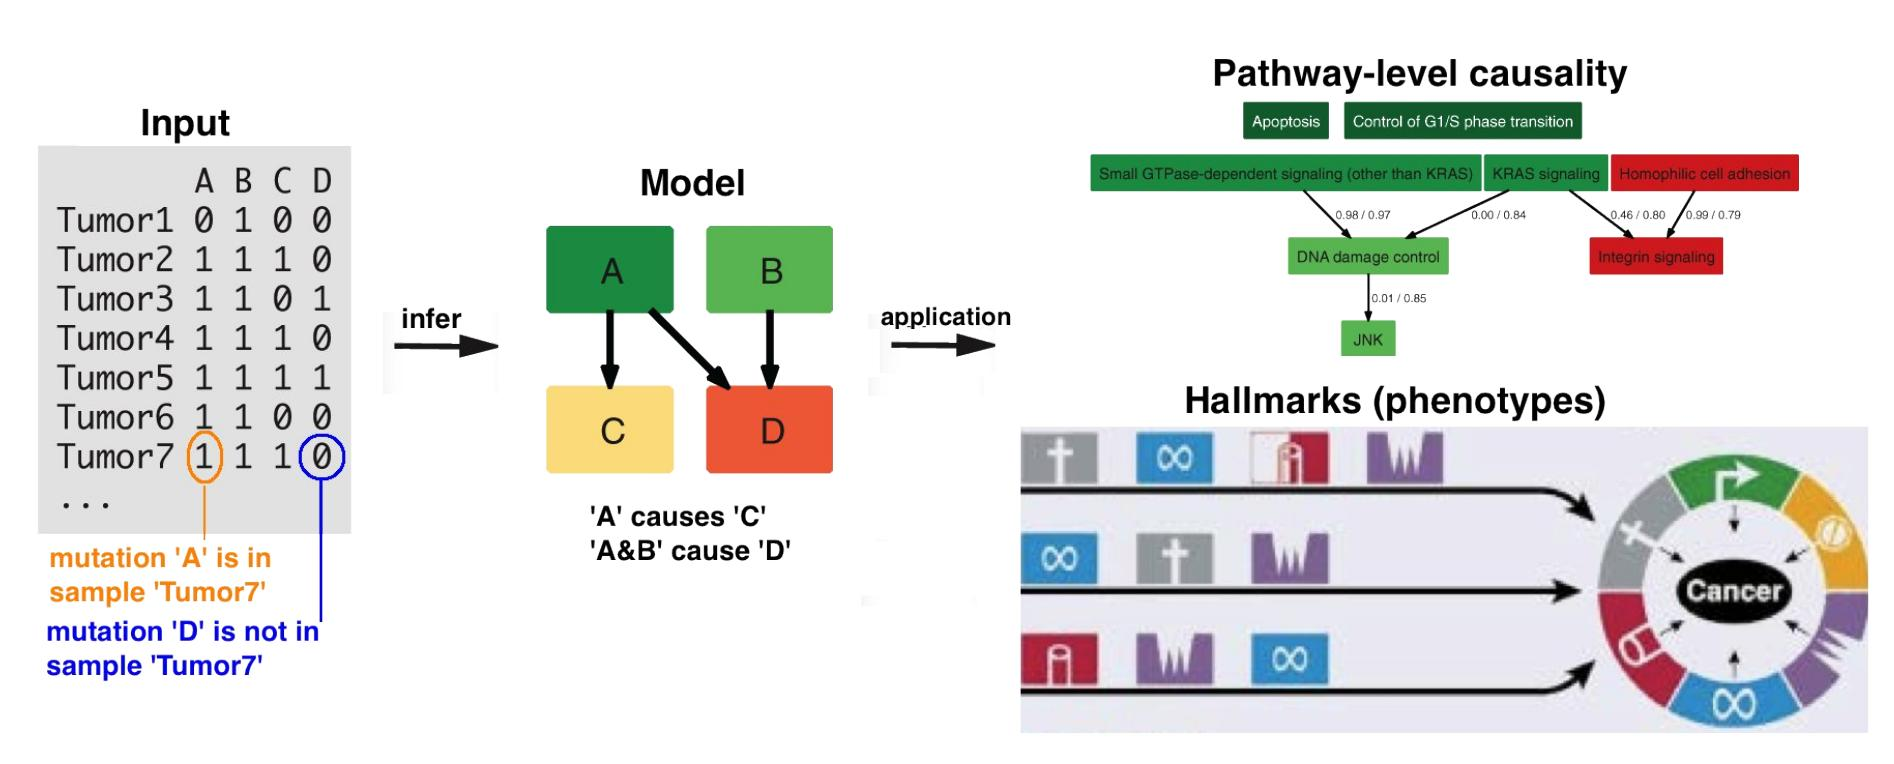
\includegraphics[scale = 0.185]{img/q1.jpg}
  \caption{Schema rappresentativo di quanto si ottiene a partire da una matrice
    booleana per studiare la ricostruzione di modelli di progressione.}
  \label{fig:q1}
\end{figure}
\subsubsection{Secondo Quesito}
Per il secondo quesito bisogna citare nuovamente le banche dati pubbliche per i
dati relativi al cancro, tra cui:ì
\begin{itemize}
  \item The Cancer Genome Atlas (\textit{TCGA})
  \item International Cancer Genome Consortium (\textit{ICGC})
\end{itemize}
Tutte queste banche dati rispondono al problema della centralizzazione dei dati
e delle informazioni, che fino a qualche anno fa erano anche parecchio
costosi.\\
Direttamente collegato è anche il tema centrale della \textit{gestione dei dati
  sperimentali}, avendo che essi devono:
\begin{itemize}
  \item essere ben catalogati
  \item essere facilmente accessibili e studiabili
  \item garantire interoperabilità
  \item garantire conformità con gli standard
  \item etc$\ldots$
\end{itemize}
e tutte queste sono tematiche prettamente computazionali.\\
Ovviamente in ottica di studio del cancro le informazioni più interessanti delle
banche dati, tra le tante informazioni disponibili, sono quelle relative alle
mutazioni, che sono di solito ereditate e persistenti tra generazioni successive
di cellule tumorali (\textit{questa è una sorta di assunzione}). Le mutazioni
più interessanti sono solitamente quelle di carattere \textit{somatico}, ovvero
le \textbf{mutazioni somatiche}. Inoltre si più dire che La probabilità di
insorgenza di una data alterazione/mutazione è correlata a quanto funzionale è
allo sviluppo del tumore, avendo quindi che si hanno le mutazioni dette
\textit{driver} e quelle dette \textit{passenger}, oltre a diversi tassi di
mutazione tumorale (\textit{anche questa è una sorta di assunzione}). Ovviamente
anche le mutazioni possono essere di vario tipo:
\begin{itemize}
  \item i cosiddetti \textbf{single nucleotide variant (\textit{SNP})}, ovvero
  mutazioni su singole basi
  \item le \textbf{perdite di eterozigosità}, con perdite di regioni genomiche,
  perdite di porzioni più piccole, mutazioni copy-number etc$\ldots$
  \item intere \textbf{delezioni} che siano terminali o interne alla sequenza
  \item \textbf{duplicazioni} di parti di sequenze che possono portare a
  \textbf{tandem}, dove le duplicazioni si appaiano una accanto all'altra, o a
  duplicazioni dove le porzioni duplicate sono separate tra loro da un'altra
  porzione di genoma
  \item \textbf{amplificazioni} di porzioni genomiche di tipo
  \textbf{intra-cromosomico} e \textbf{inter-cromosomico}
  \item \textbf{duplicazione dell'intero genoma}
\end{itemize}
\subsubsection{Terzo Quesito}
In merito al terzo quesito ci viene incontro la letteratura degli ultimi
vent'anni e oltre. Si sono studiati infatti vari tipi di modelli:
\begin{itemize}
  \item \textbf{modelli ad albero}\footnote{Desper, Papadimitriou Schäffer et
    al, 1999, 2000}, soprattutto all'inizio quando si avevano dati molto
  ``grezzi'' con grosse alterazioni. Tali modelli erano in primis basati sulle
  correlazioni. Un esempio potrebbe essere il seguente\footnote{Olde Loohuis et
    al, 2014, originally from Desper et al, 1999}, dove si ha un esempio di
  progressione cancerogena (nel dettaglio sul cancro ovarico ) rappresentata
  tramite albero:
  \begin{figure}[H]
    \centering
    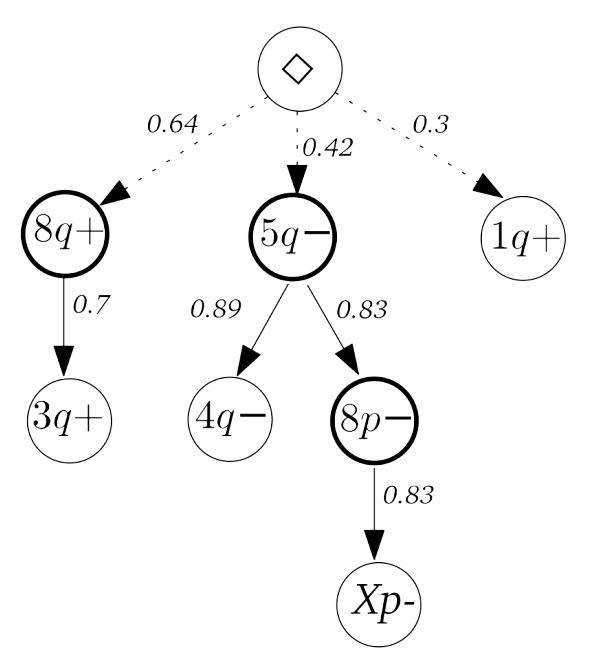
\includegraphics[scale = 0.25]{img/ovt.jpg}
  \end{figure}
  \item \textbf{modelli congiunti}\footnote{Beerenwinkel, Sturmfelds et al,
    2005, 2006, 2007}, basati principalmente su modelli Bayesiani. Un esempio
  potrebbe essere il seguente\footnote{Beerenwinkel et al, 1999} ottenuto per
  progressione congiuntiva ricostruita da un set di dati sulla risposta ai
  farmaci dell'HIV:
  \begin{figure}[H]
    \centering
    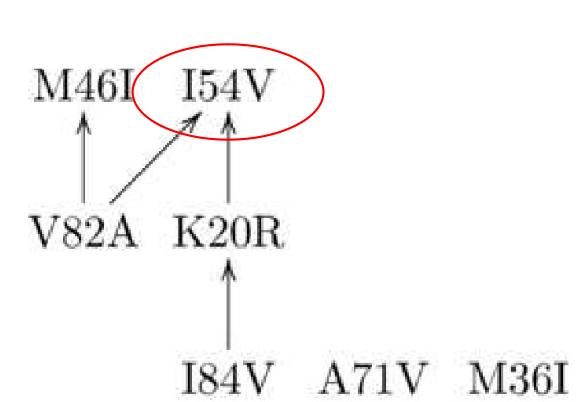
\includegraphics[scale = 0.25]{img/ovc.jpg}
  \end{figure}
  \item \textbf{modelli DAG}, che sono una generalizzazione dei due modelli
  precedenti 
\end{itemize}
\subsection{Algoritmo CAPRI}
\begin{shaded}
  Quanto trattato in merito a \textbf{TRONCO}, \textbf{CAPRESE} e \textbf{CAPRI}
  è ritrovabile nei seguenti articoli:
  \begin{itemize}
    \item D. Ramazzotti, G. Caravagna, L. Olde-Loohuis, A. Graudenzi,
    I. Korsunsky, G. Mauri, M. Antoniotti, and B. Mishra, “CAPRI: Efficient
    Inference of Cancer Progression Models from Cross-sectional Data.,”
    Bioinformatics, p. btv296, May 2015.
    \item L. O. Loohuis, G. Caravagna, A. Graudenzi, D. Ramazzotti, G. Mauri,
    M. Antoniotti,  and B. Mishra, “Inferring Tree Causal Models of Cancer
    Progression with Probability Raising,” PLoS ONE, vol. 9, no. 10, p. e108358,
    Oct. 2014.
    \item L. De Sano, G. Caravagna, D. Ramazzotti, A. Graudenzi, G. Mauri,
    B. Mishra, and M. Antoniotti, “TRONCO: an R package for the inference of
    cancer progression models from heterogeneous genomic data.,” Bioinformatics,
    p. btw035, Feb. 2016. 
    \item G. Caravagna, A. Graudenzi, D. Ramazzotti, R. Sanz-Pamplona, L. De
    Sano, G. Mauri, V. Moreno, M. Antoniotti, and B. Mishra, “Algorithmic
    methods to infer the evolutionary trajectories in cancer progression,”
    Proc. Natl. Acad. Sci. U.S.A., pp.  201520213–10, Jun. 2016.
  \end{itemize}
\end{shaded}
Si approfondiscono ora alcune delle tecniche sviluppate nel laboratorio di
ricerca \textit{BIMIB}, ora \textit{DCB}:
\begin{itemize}
  \item in primis è stato sviluppato l'algoritmo detto \textbf{CAncer
    PRogression Extraction with Single Edges (\textit{CAPRESE})}, per la
  modellazione tramite alberi
  \item si è poi lavorato sull'algoritmo \textbf{CAncer PRogression Inference
    (\textit{CAPRI})}, un'estensione di \textit{CAPRESE} per lavorare tramite
  modelli \textit{DAG}. Approfondiremo sopratutto questo
  \item questi algoritmi, più altre funzionalità di supporto, come l'accesso a
  \textit{cBIO} e \textit{TCGA}, sono state raccolte nella libreria per il
  linguaggio $R$ detta \textbf{Translational ONCOlogy
    (\textit{TRONCO})}. L'algoritmo in grado di ricostruire un DAG
  rappresentativo delle possibili progressioni di un tumore, intese come
  accumuli di eventi diversi, il \textit{DAG} prodotto è un riassunto delle
  possibili progressioni osservabili in una popolazione  
\end{itemize}
partiamo da un esempio molto sintetico. Si supponga di voler modellare una
progressione tumorale in cui avvengono in primis due mutazioni, una detta
\textit{EGFR} e, poi, una detta \textit{CDK}. Si devono fare due importanti
assunzioni, abbastanza forti per di più, per poter procedere con la
modellazione: 
\begin{enumerate}
  \item \textbf{assunzione di persistenza}, ovvero le mutazioni acquisite non
  scompaiono (\textit{e questo non è vero per le espressioni geniche e gli
    effetti epigenetici}). Si ha quindi, riprendendo l'esempio, che con la
  mutazione \textit{EGFR} si acquisisce un vantaggio selettivo e si procede
  quindi con l'espansione clonale, aumentando anche la probabilità di acquisire
  una mutazione \textit{CDK}. Quando si hanno entrambe le mutazioni si ha una
  specie selettivamente ancora più avvantaggiata
  \item \textbf{assunzione di selezione di eventi}, ovvero gli eventi rilevanti
  per la progressione devono essere scelti in anticipo. In pratica, riferendoci
  all'esempio, si sa già che bisogna studiare un modello con in input le
  mutazioni \textit{EGFR} e \textit{CDK}. Limitarsi a poche combinazioni di
  eventi rende la ricostruzione computazionalmente più fattibile, non usando
  quindi l'intera moltitudine di dati provenienti dagli studi oncologici. Si fa
  quindi una sorta di \textit{studio supervisionato}, che nel dettaglio viene
  fornito da vari tool ormai standard atti soprattutto a scovare le mutazioni
  \textit{driver} 
\end{enumerate}
Un'altro aspetto fondamentale in questo studio è che ogni paziente ha una sua
storia di evoluzione e progressione cancerogena diversa.  L'effettivo input
all'algoritmo di ricostruzione della progressione può essere pensato come un
insieme di possibili traiettorie, cioè di sequenze di alterazioni genomiche che
si accumulano in modo diverso, bisogna quindi procedere con il conteggiare e
assegnare le giuste probabilità ad ogni singola occorrenza di un evento.\\
Si sono sviluppati vari modi negli anni per ricostruire modelli ad alberi o DAG
e utti gli algoritmi necessitano di una misura per decidere se e come includere
un arco nella ricostruzione. Vediamo quindi come si è scelto di procedere in
\textit{BIMIB/DCB}, che si basa sulla \textbf{teoria della causalità
  probabilistica}. \\
Un primo punto cardine considerato è infatti quello della \textbf{teoria della
  causalità} di Suppes, un filosofo e matematico. In biologia bisogna comunque
considerare che aggiungere dei concetti di causalità complicano molto i modelli,
anche se con questa teoria si riesce ad ottenere in modo implicito l'idea di
\textbf{direzionalità temporale} nei modelli. Il nucleo di questa teoria è molto
semplice. Dati due eventi $c$ ed $e$, occorrenti rispettivamente al tempo $t:c$
e $t_e$, con:
\[0<P(c)\mbox{ e } P(e)<1\]
si ha che $c$ è detto \textbf{causa \textit{prima facie}} per $e$ se si
rispettano due proprietà:
\begin{enumerate}
  \item la \textbf{proprietà di priorità temporale}, ovvero banalmente:
  \[t_c<t_e\]
  che garantisce un ordine temporale tra gli eventi
  \item la \textbf{proprietà della crescita delle probabilità}, che ci dice che
  la probabilità che l'evento $e$ accada essendo accaduto l'evento $c$ sia
  maggiore (e preferibilmente molto maggiore) di quella in cui non si ha
  l'evento $c$:
  \[P(e | \neg c) < P(e | c)\]
\end{enumerate}
Queste due proprietà, \textbf{necessarie ma non sufficienti}, garantiscono la
direzionalità del modello.\\
Oltre alla teoria di Suppes si ha anche che sia le misurazioni che le analisi
teoriche vengono reinterpretate in termini biologicamente plausibili,
eventualmente anche ridefinendo le  relazioni di vantaggio selettivo. Queste
scelte permettono di racchiudere maggiori informazioni negli algoritmi proposti
da \textit{BIMIB/DCB} di ricostruzione, che mostrano ottime prestazioni rispetto
allo stato dell'arte, ora spesso basati su modelli Bayesiani o sui modelli
causali di Pearl.\\
Approfondiamo quindi meglio le basi per la ricostruzione del modello di
progressione.\\
Le già anticipate cause \textit{prima facie} possono essere di due tipologie:
\begin{itemize}
  \item \textbf{autentiche/genuine}, quelle ``corrette''
  \item \textbf{spurie}, quelle ``errate''
\end{itemize}
e per questo le due condizioni risultano solo sufficienti e non
necessarie. Inoltre, parlando di dati \textit{cross-sectional},  la priorità
temporale tra gli eventi non è nota, quindi il problema della ricostruzione
diventa più difficile. Il problema diventa quindi come stabilire se un dato
arco tra due eventi corrisponda o meno a una causa spuria, e quindi non
vada considerato, avendo comunque che l'interpretazione di un arco sarà quella
di una relazione di vantaggio selettivo tra eventi genetici. \\
Inoltre un'ulteriore complicazione è data dal fatto che nulla assicura che si
parli solo di due eventi ma si possono avere combinazioni complesse di causalità
tra eventi e per questo nell'algoritmo \textit{CAPRI} queste situazioni vengono
gestite tramite \textbf{formule booleane}, come le formule congiuntive del tipo
utilizzato nelle reti Bayesiane congiuntive. Si distinguono quindi:
\begin{itemize}
  \item \textbf{singleton}, dove una mutazione accade prima di un'altra e si ha
  relazione causale
  \item \textbf{co-occorrenze}, dove più di una mutazione accade prima di
  un'altra e si ha relazione causale. Ovviamente in questo caso la complessità
  aumenta 
\end{itemize}
Nell'algoritmo \textit{CAPRI} si ha anche una condizione finale, ovvero la
condizione per la seleziona vantaggiosa tramite \textit{patterns} (indicando con
$\triangleright$ la corretta causalità):
\[c\triangleright e\iff P(c)>P(e)\land P(e|c)>P(e\neg c)\]
Si parte quindi da un modello causale con i vantaggi selettivi, si fanno le
osservazioni sulle \textit{regolarità imperfette} e si fanno studi di frequenza. 
Più nel profondo l'inferenza dei risultati viene poi ottenuta, ad esempio,
tramite tecniche statistiche come:
\begin{itemize}
  \item \textbf{boostrap}, una tecnica statistica di ricampionamento con
  reimmissione per approssimare la distribuzione campionaria di una
  statistica. Permette perciò di approssimare media e varianza di uno stimatore,
  costruire intervalli di confidenza e calcolare \textit{p-value} di test
  quando, in particolare, non si conosce la distribuzione della statistica di
  interesse
  \item \textbf{test del \textit{p-value}} e altri test
\end{itemize}
Si ottengono quindi relazioni causali tra mutazioni, eventualmente anche con
l'effetto co-occorrente (e quindi senza avere interesse sull'ordine) di più
mutazioni che causano una terza mutazione. Ad esempio se si ha una mutazione $A$
e una mutazione $B$ che causano in modo co-occorrente la mutazione $C$ si ha, dal
punto di vista statistico:
\[\min\{P(A),P(B)\}>P(C)\land P(C|A,B)>P(C|\neg(AB))\]
Per pattern complessi si è studiato sperimentalmente come l'algoritmo
\textit{CAPRI} che è in grado di capire la causalità tra varie mutazioni e
rappresentarle tramite formule booleane. La complessità del modello poi si
riconduce alla complessità di tali formule, ottica dei vari studi teorici sulla
complessità di \textit{SAT} etc$\ldots$.\\
Le formule booleane sono della forma \textbf{conjunctive normal form
  (\textit{CNF})}, ovvero una congiunzione di clausole, dove le clausole sono
una disgiunzione di letterali.\\ 
In ottica di limitare la complessità dobbiamo quindi evidenziare le relazioni
\textit{autentiche} più significative in quanto l'algoritmo
\textit{naive} individuerebbe anche transitività, sotto-formule e altri archi
topologici come possibili relazioni di selettività. Un esempio è mostrato in
figura \ref{fig:gvss}.\\
\begin{figure}
  \centering
  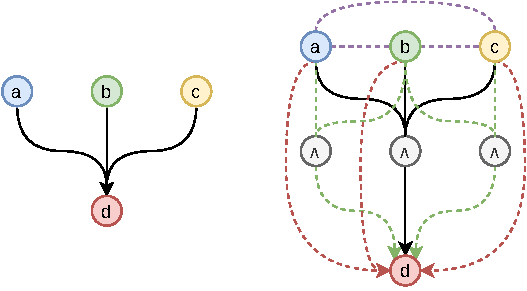
\includegraphics[scale = 1.4]{img/gvss.pdf}
  \caption{Test case di confronto tra una progressione reale a sinistra (dove i
    collegamenti sottintendono la congiunzione) e una selezione 
    co-occorrente a destra per rappresentare la formula
    $a\land b\land c\triangleright d$. Con le frecce piene si rappresentano le
    relazioni ``reali'', quelle autentiche, con le frecce tratteggiate rosse
    e verdi, rispettivamente, transitività e sotto-formule, che sono una via di
    mezzo tra relazioni autentiche e relazioni spurie ma comunque eliminabili,
    mentre con le righe tratteggiate viola gli archi topologici, che sono la
    massima rappresentazione di relazioni spurie.} 
  \label{fig:gvss}
\end{figure}
L'\textit{algoritmo CAPRI} è una combinazione di sei passaggi che sono
responsabili della produzione di un insieme di relazioni di selettività e della
successiva pulizia del modello generato:
\begin{enumerate}
  \item una prima fase gestione dei dati in input
  \item una fase di preprocessing con aggiunta di informazioni, sotto forma di
  \textit{CNF}, detta \textbf{lifting}, al modello grezzo 
  ottenuto dai dati. Si ha un insieme $G$ di $n$ eventi provenienti da $m$
  samples \textit{cross-sectional}, avendo quindi una matrice booleana $n\times
  m$. Si assume in questa un insieme di ipotesi:
  \[\Phi=\{\phi_i\triangleright e_i|\,\,\,1\leq i\leq k\}\mbox{, con }k+n\ll m\]
  Ogni singolo $\phi_i\triangleright e_i$ è usato per accresce la matrice in
  input ottenendo una matrice $D(\Phi)$ che codifica le relazioni di selettività
  opzionali come eventi
  \item una fase di selezione dei nodi del \textit{DAG}
  \item una prima fase di selezione degli archi del \textit{DAG}
  \item si ha poi una fase di etichettamento degli archi. In questa fase e
  relazioni di selettività codificate sono formule 
  \textit{CNF}, quindi possono essere trattate in modo composito verificando
  separatamente ogni congiunzione (ovvero una disgiunzione).\\
  L'algoritmo include nella costruzione archi tra due eventi $c$ e $e$ sse:
  \[P(c)-P(e)>0\land P(e|c)-P(e|\neg c)>0\]
  e questa è la condizione principale. Si noti che le probabilità sono stimate
  dai dati direttamente, tramite un primo step di \textit{boostrap}. Il
  \textit{DAG} ricostruito contiene tutte le corrette relazioni di selettività
  ma anche parecchie spurie, che non vengono ancora eliminate. Ogni arco è
  etichettato con una probabilità che è essenzialmente la probabilità di
  osservare un certo profilo mutazionale in un campione. \\
  Già alla fine di questa fase il modello ricostruito è interpretabile dal punto
  di vista grafico, tramite varie librerie esterne 
  \item si ha infine una fase di \textit{likelihood fit}. Ricordando che le
  assunzioni di Suppes sono solo necessarie per ``filtrare'' le relazioni
  spurie, ovvero i falsi positivi che sono stati inclusi nei passaggi
  precedenti, calcoliamo un \textit{fit di massima verosimiglianza} che include
  un termine di regolarizzazione, termine che può essere scelto e calcolato in
  modo diverso. Ad esempio come criteri si hanno attualmente
  nell'\textit{algoritmo CAPRI}: 
  \begin{itemize}
    \item \textbf{Bayesian Information Criterion (\textit{BIC})}, più
    conservativo
    \item \textbf{Akaike Information Criterion (\textit{AIC})}
  \end{itemize}
  questa scelta permette quindi vari \textit{tradeoff}.\\
  Infine si usa un passaggio di \textit{bootstrap} per dedurre gli intervalli
  di confidenza per ciascuna relazione di selettività dedotta. 
\end{enumerate}
L'\textit{algoritmo CAPRI} (ma anche in primis l'\textit{algoritmo CAPRESE})
è \textbf{corretto} e \textbf{completo}, avendo che sono riportate tutte e sole
le vere relazioni di selettività desumibili dai dati. Dal punto di vista
computazionale invece si nota come gli step più onerosi sono la fase di
preprocessing dei dati, ad esempio il parsing dei file \textit{MAF}, e le due
fasi di \textit{boostrap}.\\
Va sempre ricordato che le relazioni di precedenza che l'algoritmo
deduce non spiegano le cause meccanicistiche biochimiche di un modello di
progressione, infatti l'algoritmo fa solo un'affermazione sul fatto che
l'osservazione di un dato insieme di mutazioni aumenta la probabilità di vederne
uno successivo (\textbf{questa osservazione è fondamentale}).\\
Un altro vantaggio dell'\textit{algoritmo CAPRI} è la gestione del
\textit{rumore}, migliore di altre soluzioni allo stato dell'arte. Si hanno
comunque molti altri punti di forza rispetto ad altre soluzioni, tra le quali si
annoverano:
\begin{itemize}
  \item \textbf{Incremental Association Markov Blanket (\textit{IAMB})} e
  \textbf{PC}, per quanto riguarda soluzioni strutturali
  \item \textbf{Bayesian Information Criterion (\textit{BCI})} e
  \textbf{Bayesian Dirichlet (\textit{BDE})}, per quanto riguarda la
  soluzioni basate sulla verosimiglianza  
  \item \textbf{Conjunctive Bayesian Networks}, per quanto riguarda soluzioni
  ibride 
\end{itemize}
\textbf{Su slide lezione 10 alle pagine 39 e 40 vari grafici per la misura delle
  performance di \textit{CAPRI}}.
\subsection{Usi reali di TRONCO e CAPRI}
L'uso di \textit{TRONCO}, e quindi dell'\textit{algoritmo CAPRI} è stato usato,
ad esempio per:
\begin{itemize}
  \item lo studio della \textbf{leucemia}, nel dettaglio della \textbf{Atypical
    Chronic Myeloid Leukemia (\textit{aCML})}, a partire dai dati di 64 pazienti
  studiati con il dipartimento di Medicina della Bicocca
  \item lo studio del cancro al colon, il \textbf{Colorectal cancer
    (\textit{CRC})}, in collaborazione con l'università di Barcellona e usando
  dati di circa 200 samples presi da \textit{TCGA}
\end{itemize}
\subsubsection{Il caso Reale dello Studio della aCML}
In questo caso si è considerato un set di 64 pazienti con aCML per i quali una
\textit{mutazione puntiforme missense}, un tipo di mutazione puntiforme in cui
un aminoacido diverso è posto all’interno della proteina prodotta, diverso da
quello originale, ricorrente della proteina \textbf{SET-binding 1 
  (\textit{setbp1})}\footnote{Piazza, R., et al. (2013). Recurrent setbp1
  mutations in atypical chronic myeloid leukemia. Nature genetics, 45(1),
  18–24.}.  \\
L'analisi ha considerato:
\begin{itemize}
  \item geni selezionati in modo che fossero mutati in almeno il 5\% dei
  pazienti
  \item geni selezionati che si ipotizzava facessero parte di un
  pattern funzionale di progressione aCML (come indicato in letteratura) 
\end{itemize}
\begin{figure}
  \centering
  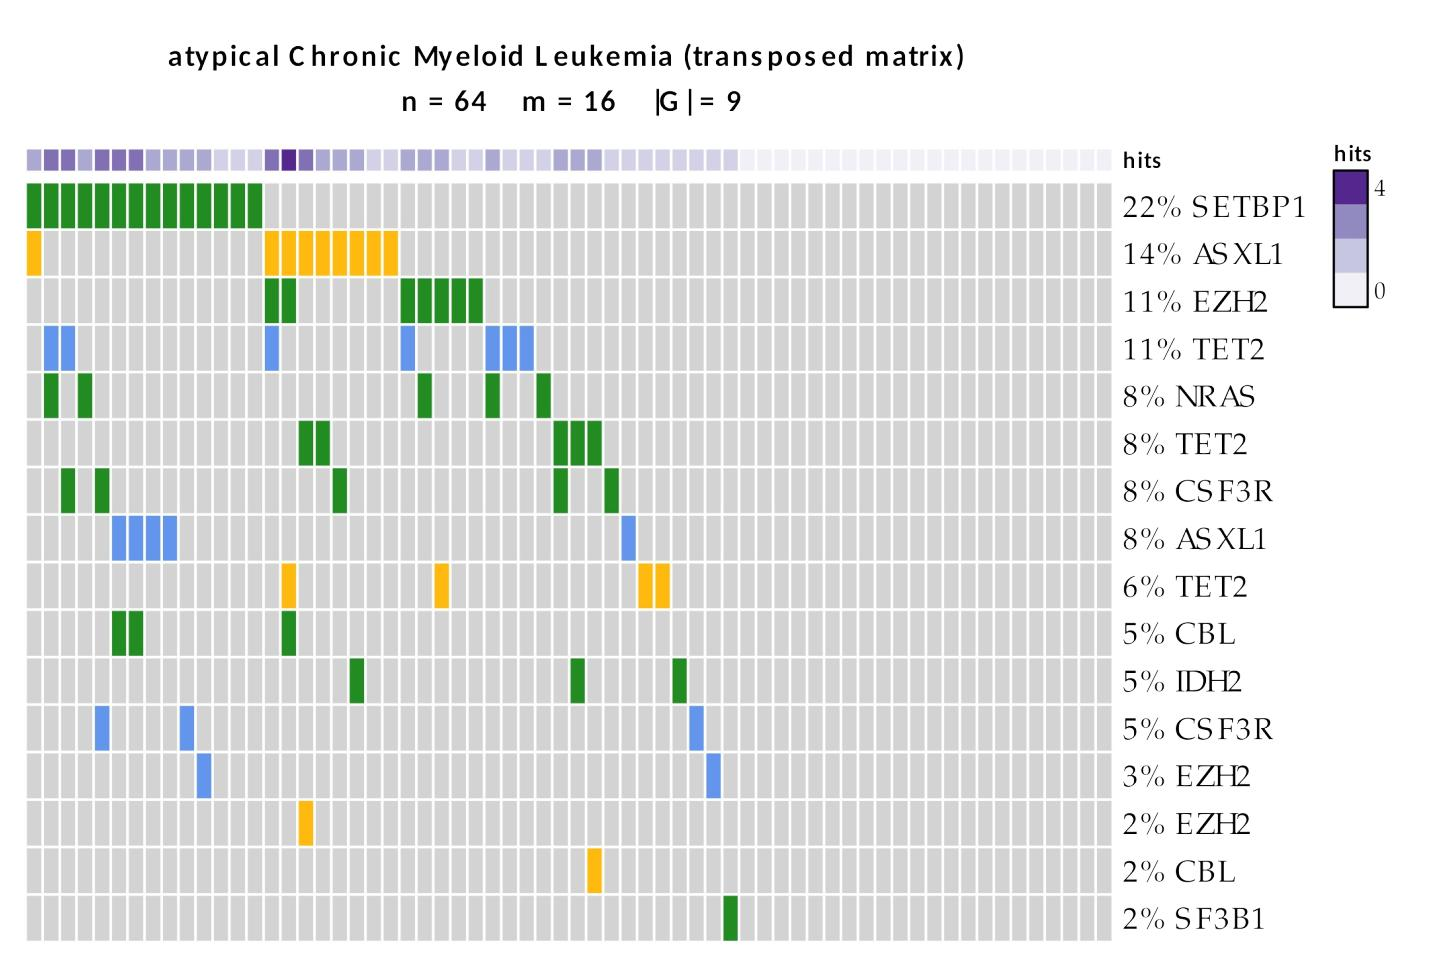
\includegraphics[scale = 0.22]{img/acml1.jpg}
  \caption{Immagine ottenuta tramite la libreria \textit{oncoprint} con una
    rappresentazione delle analisi fatte per \textit{aCML}. Ogni colonna
    rappresenta un paziente/sample mentre ogni riga una mutazione. Le mutazioni
    sono ordinate in ordine decrescente di incidenza.}
\end{figure}
In merito a questo studio sono stati formulati due rigidi vincoli di
esclusività:
\begin{enumerate}
  \item l'esclusività tra le mutazioni \textit{ASXL1} e \textit{SF3B1},
  rappresentabile tramite la formula:
  {\small{\[(\mbox{ASXL1 Nonsense point} \oplus \mbox{ASXL1 Ins/Del}) \oplus
        \mbox{SF3B1 Missense point}\] }}
  \item  l'esclusività tra le mutazioni \textit{TET2} e \textit{IDH2},
  rappresentabile tramite la formula:
  \[(\mbox{TET2 Nonsense point} \oplus \mbox{TET2 Missense point}\]\[ \oplus
    \mbox{TET2 Ins/del}) \oplus \mbox{IDH2 Missense point}\]
\end{enumerate}
Ottenendo i seguenti risultati, direttamente tramite \textit{TRONCO}:
\begin{figure}[H]
  \centering
  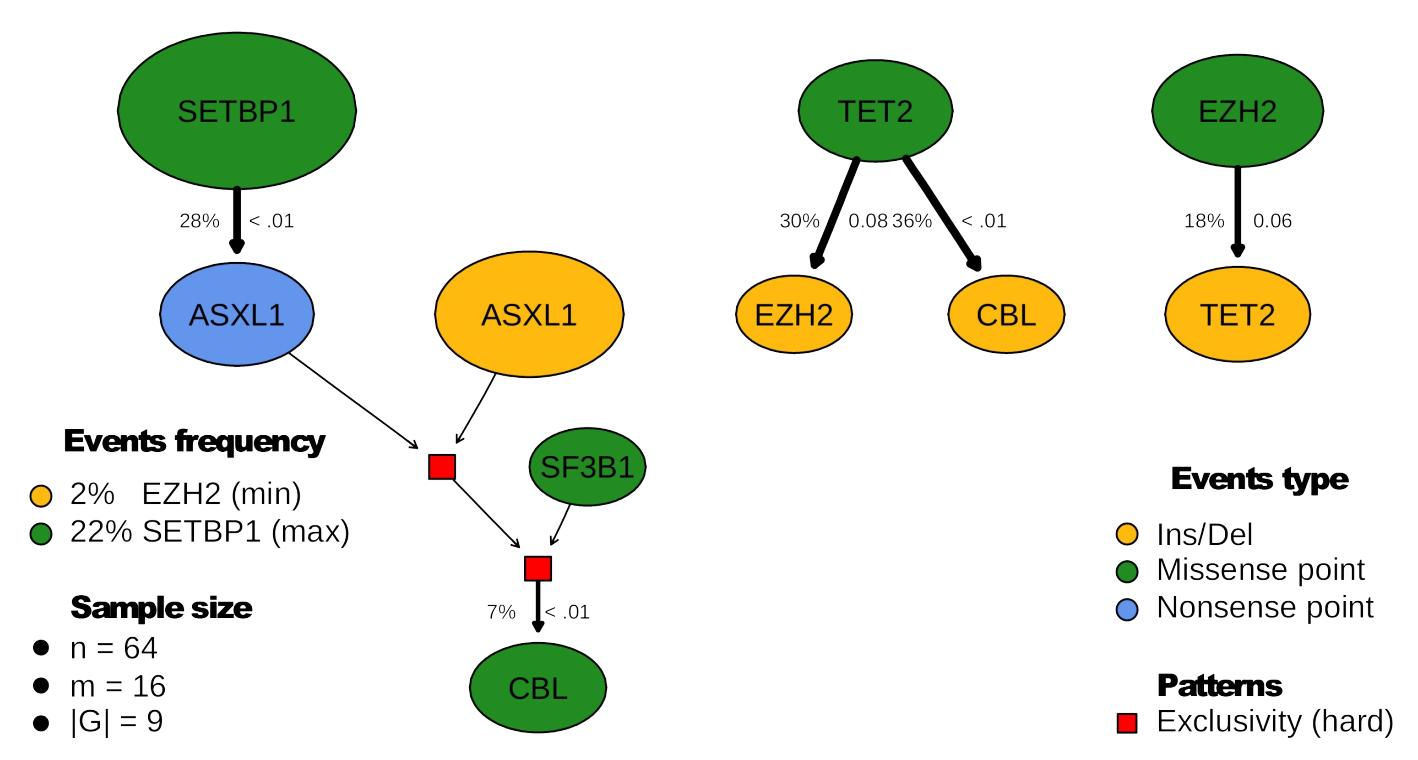
\includegraphics[scale = 0.22]{img/acml2.jpg}
\end{figure}
Alla fine l'\textit{algoritmo CAPRI} trova la seguente, tra le altre, relazione
di selettività:
{\footnotesize{\[(\mbox{ASXL1 Nonsense point} \oplus \mbox{ASXL1 Ins/del})
      \oplus \mbox{SF3B1 Missense point} \triangleright \mbox{CBL Missense
        point}\]}} 
\end{document}

% LocalWords:  clock  differenzialmente sequenziatore reference trascrivibile
% LocalWords:  REST ligandi discretizzato Petri FSA primis delay propensità
% LocalWords:  Gillespie condition silico morfogeni discretizzare pathway
% LocalWords:  randomicamente isoformi chemostato simulabilità colonscopia
% LocalWords:  replicatori microambienti microambiente Bayesiani preprocessing
% LocalWords:  etichettamento
